\documentclass[12pt, a4paper]{book}
\begin{document}\label{chap:Best_ML_MI}
\chapter{Model independent approach}
\graphicspath{{../../Plots/}}
\section{Dark Higgs Light Dark Sector}
\begin{figure}[!ht]
	\centering
	\begin{subfigure}[b]{0.49\textwidth}
      \centering
      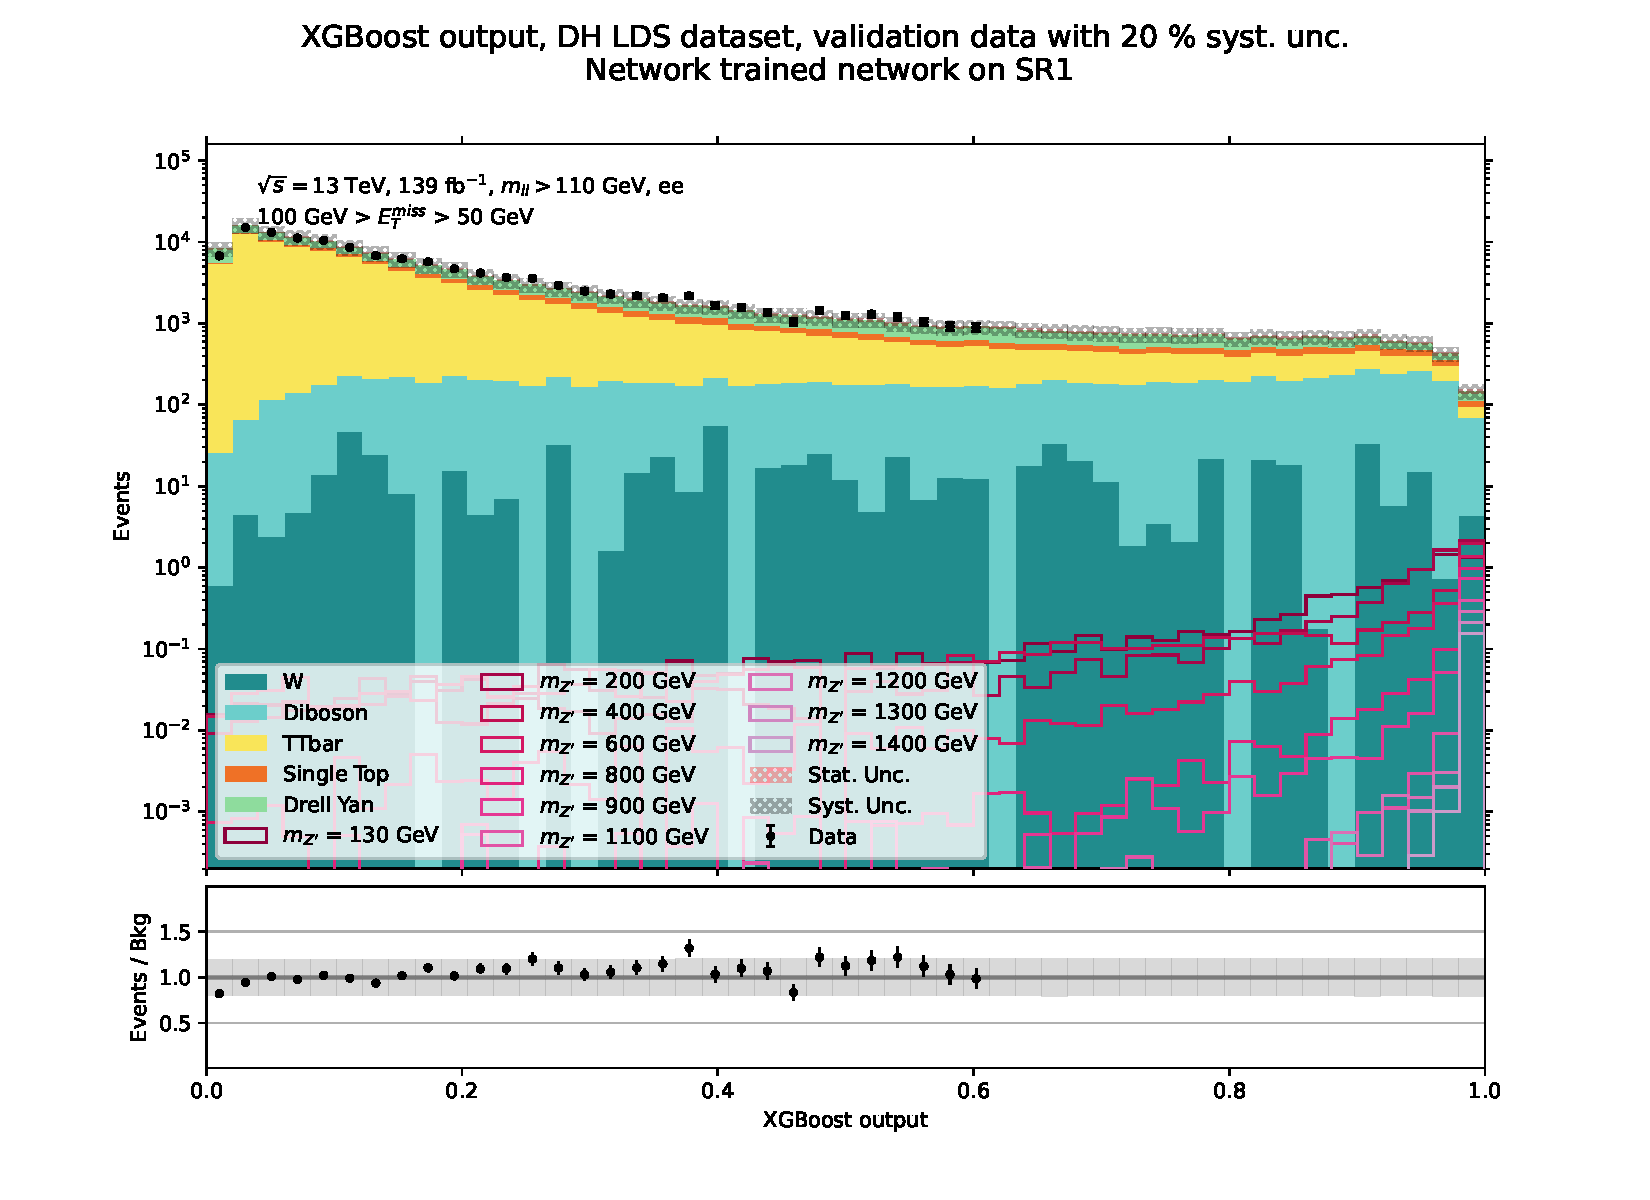
\includegraphics[width=1\textwidth]{XGBoost/Model_independent/50-100/DH_LDS/VAL_ee.pdf}
   \end{subfigure}
   \hfill
   \begin{subfigure}[b]{0.49\textwidth}
      \centering
      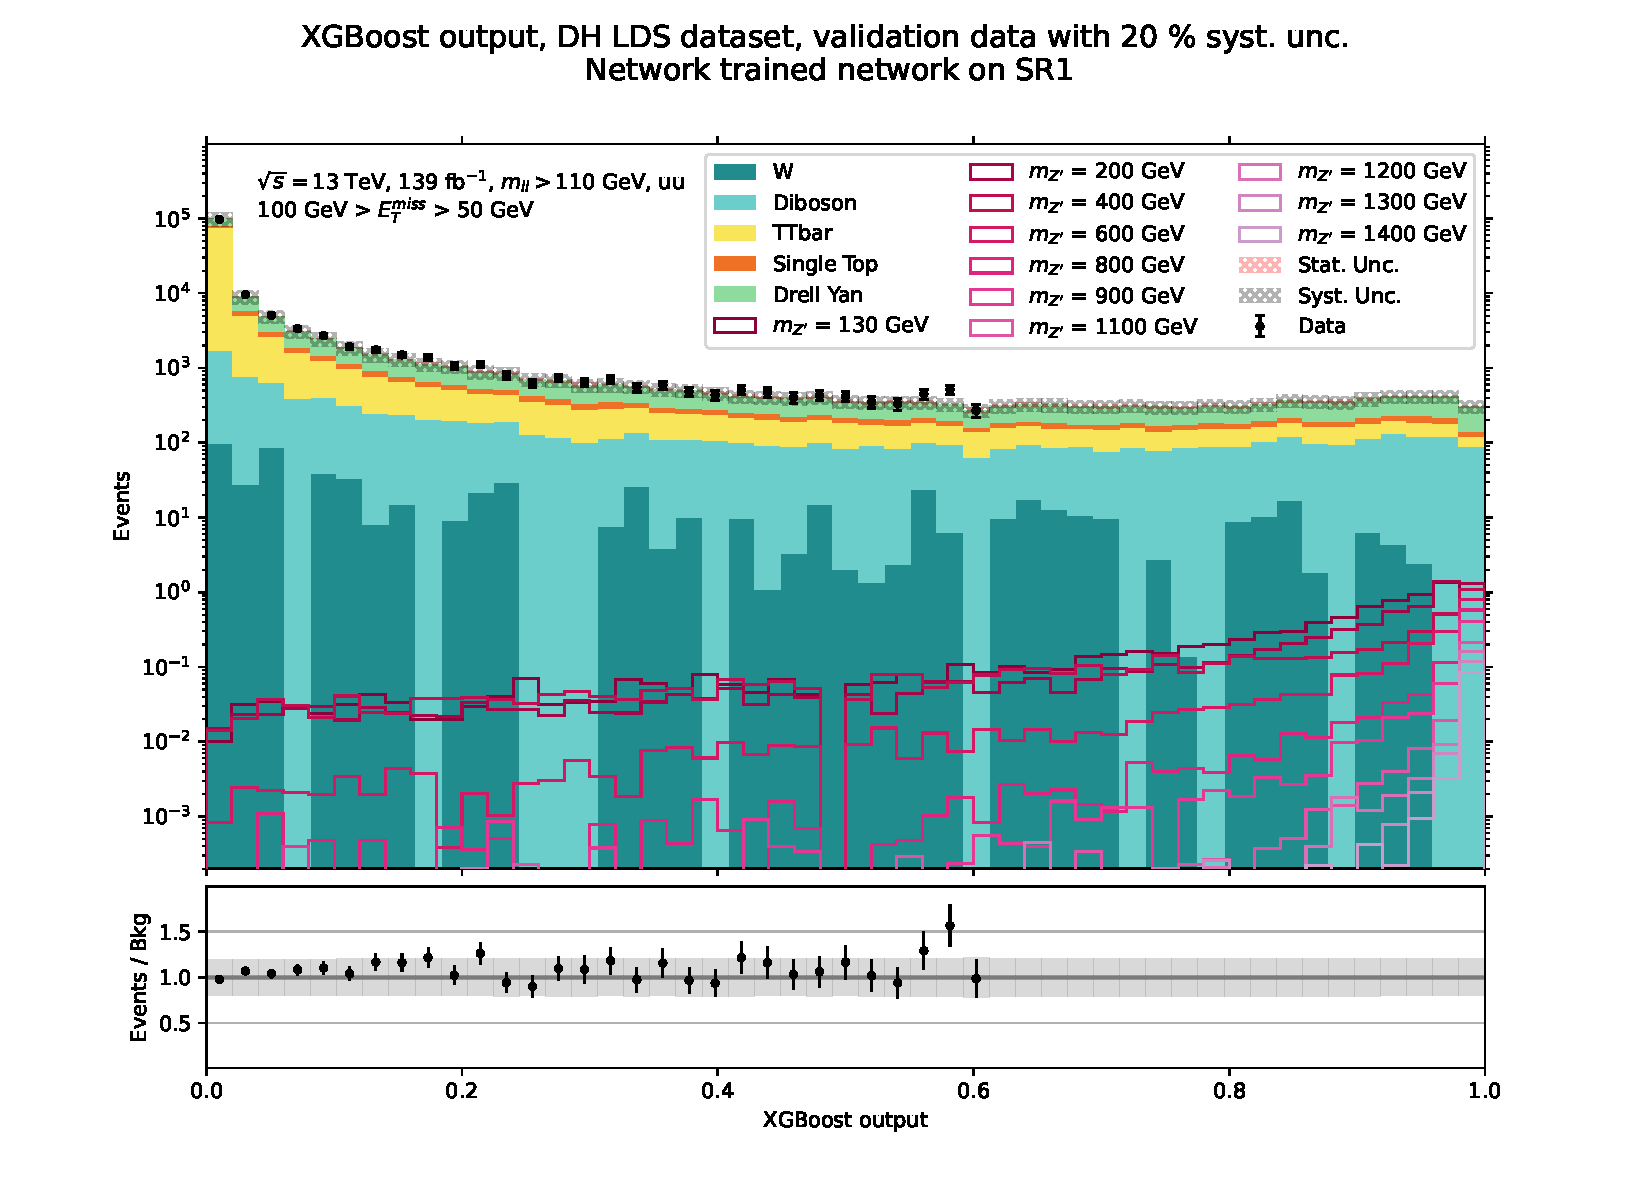
\includegraphics[width=1\textwidth]{XGBoost/Model_independent/50-100/DH_LDS/VAL_uu.pdf}
   \end{subfigure}
   \hfill
   \begin{subfigure}[b]{0.49\textwidth}
      \centering
      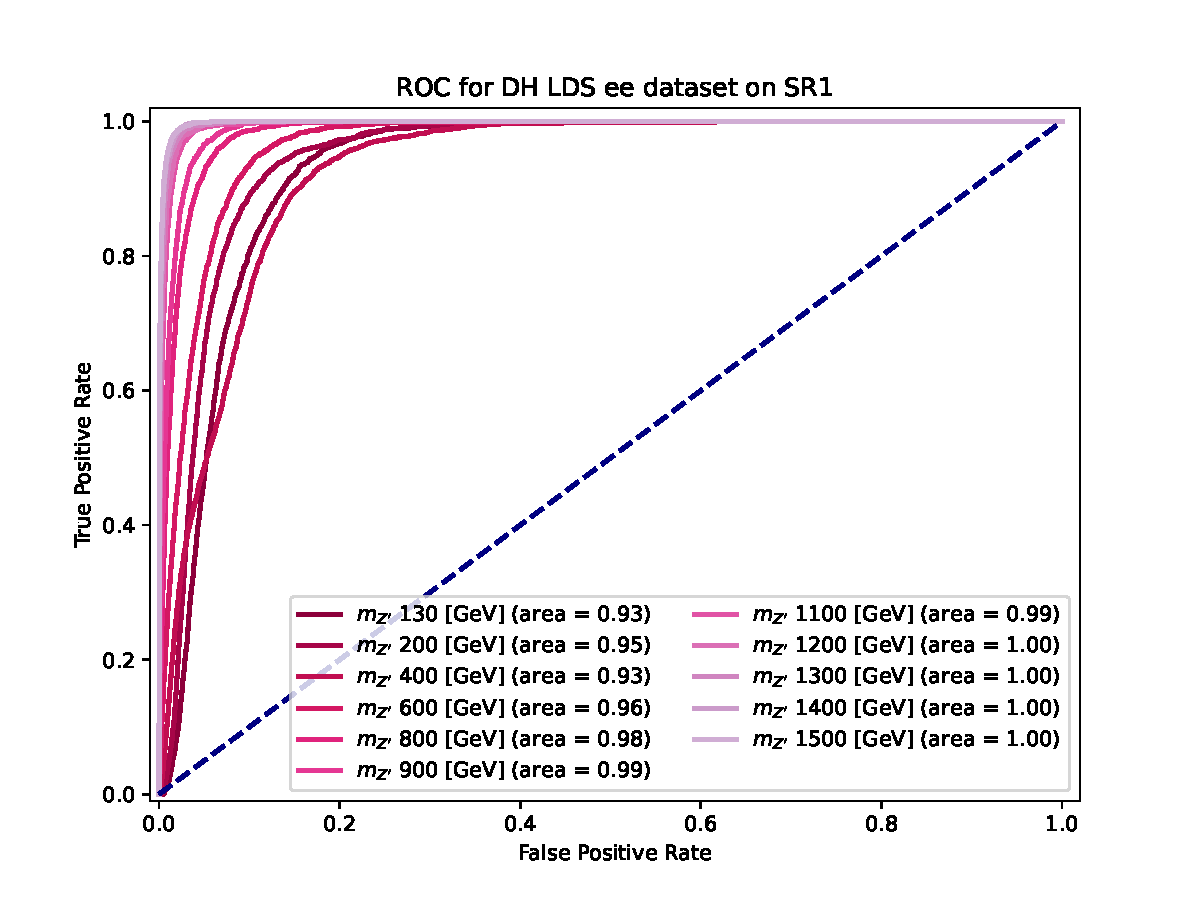
\includegraphics[width=1\textwidth]{XGBoost/Model_independent/50-100/DH_LDS/ROC_ee.pdf}
   \end{subfigure}
   \hfill
   \begin{subfigure}[b]{0.49\textwidth}
      \centering
      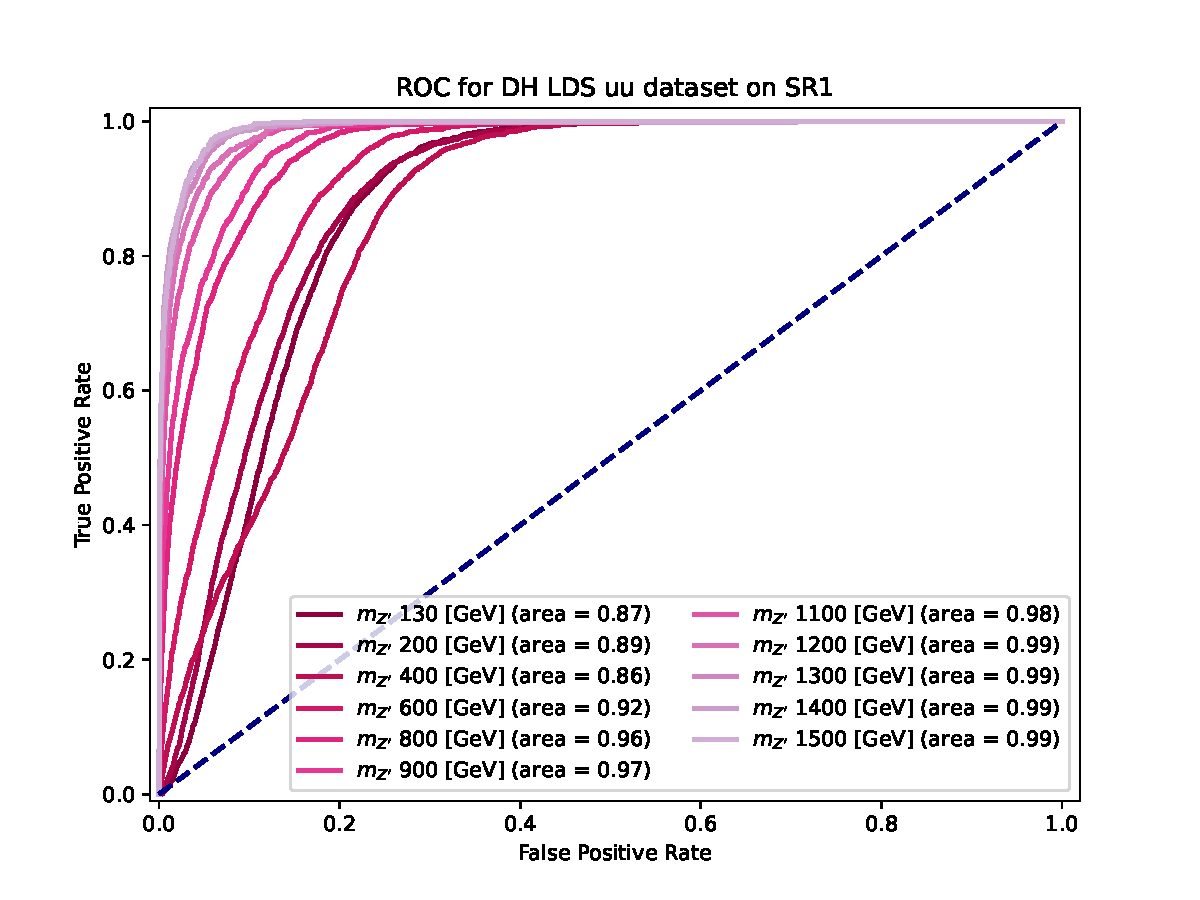
\includegraphics[width=1\textwidth]{XGBoost/Model_independent/50-100/DH_LDS/ROC_uu.pdf}
   \end{subfigure}
   \hfill
	\begin{subfigure}[b]{0.49\textwidth}
      \centering
      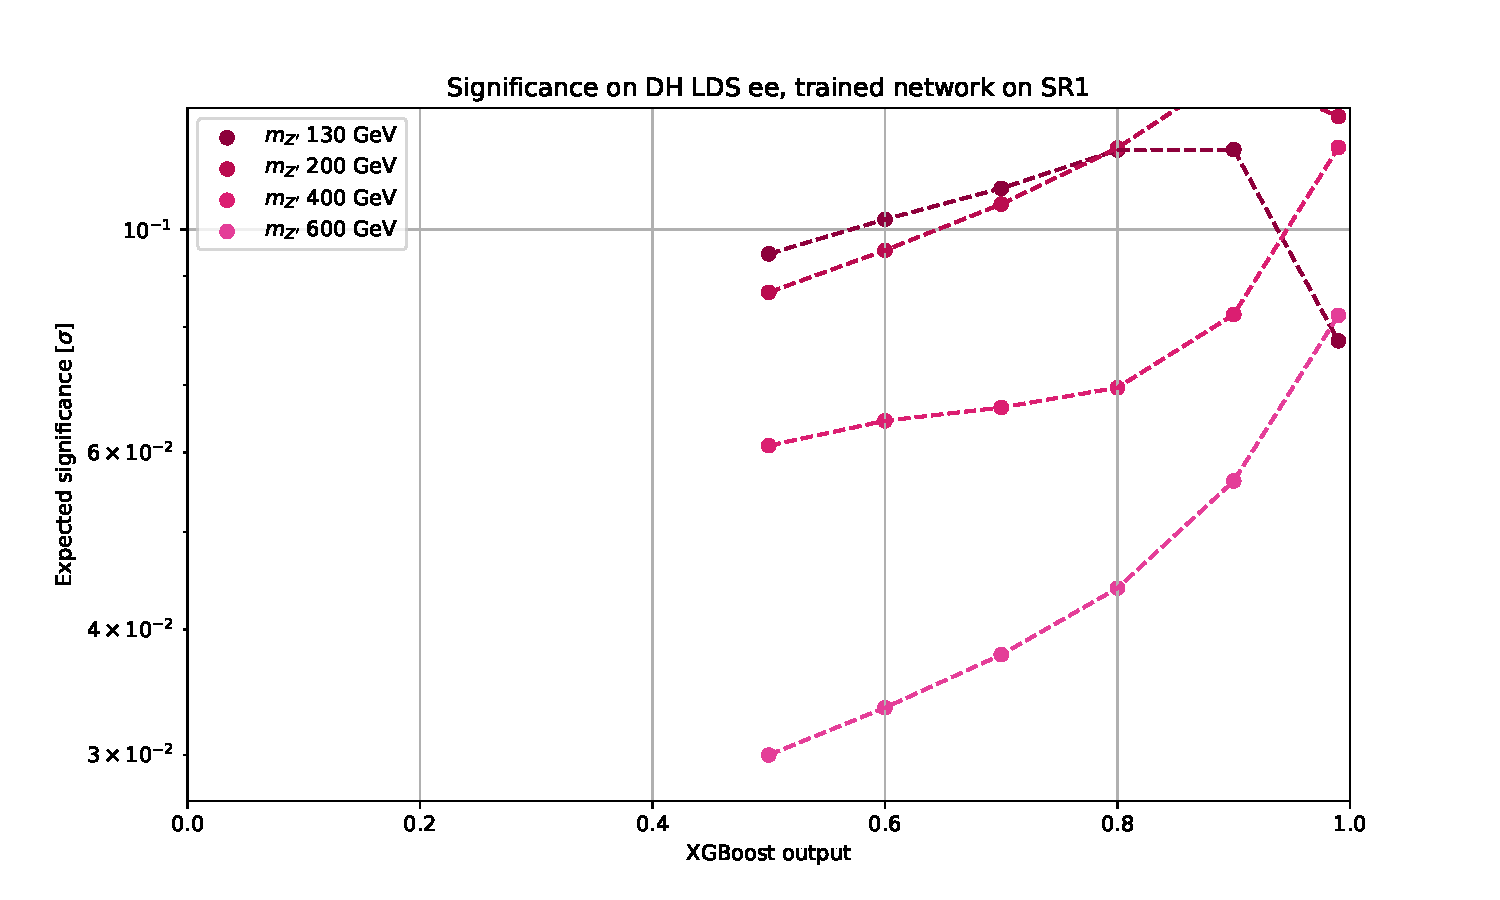
\includegraphics[width=1\textwidth]{XGBoost/Model_independent/50-100/DH_LDS/EXP_SIG_ee.pdf}
   \end{subfigure}
   \hfill
   \begin{subfigure}[b]{0.49\textwidth}
      \centering
      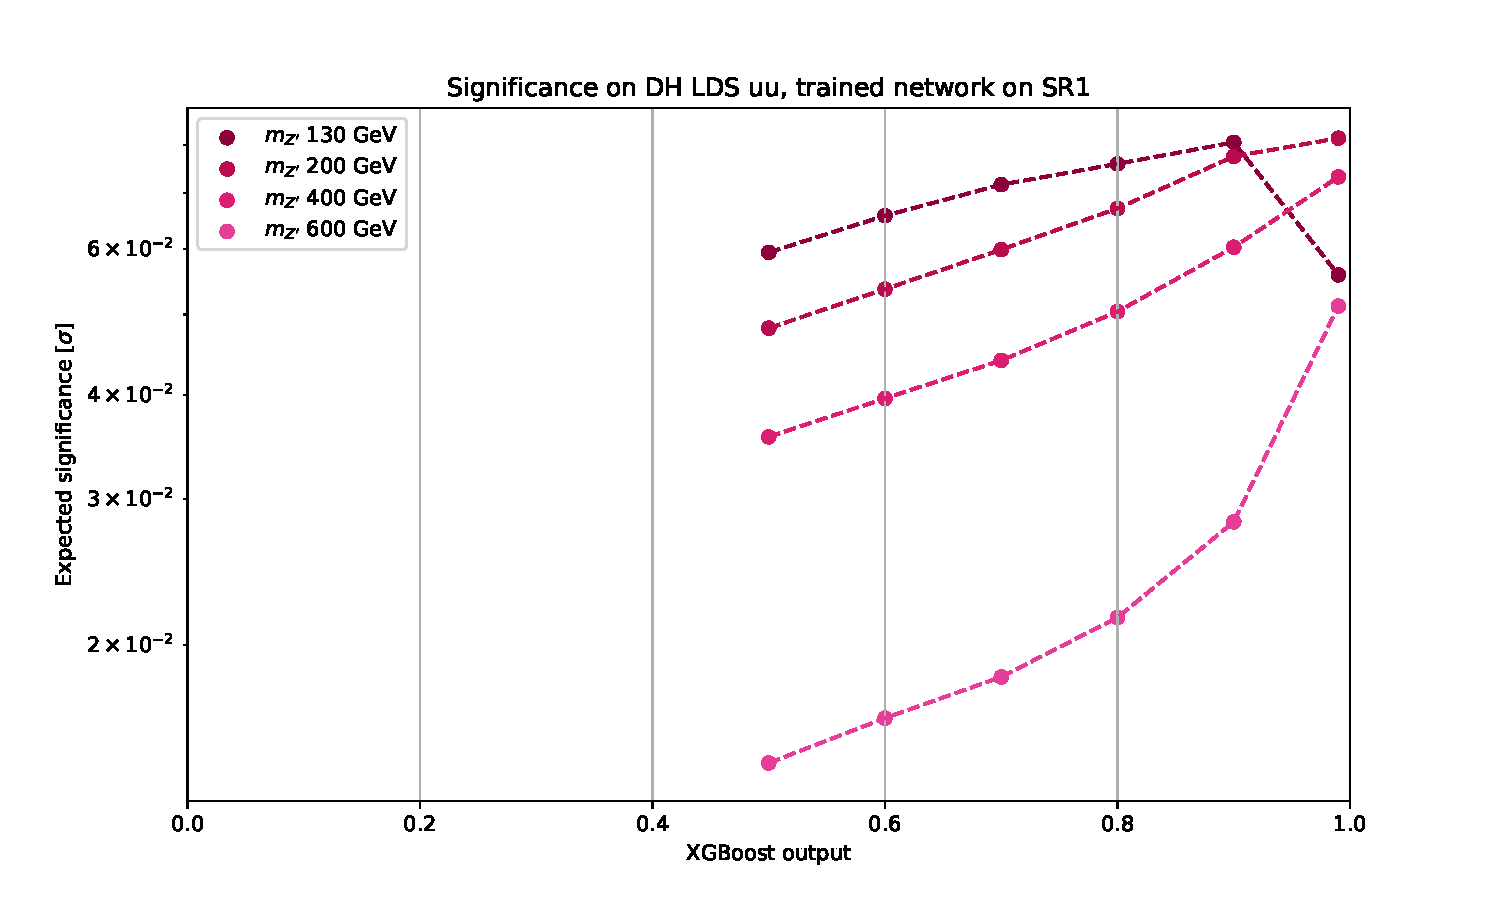
\includegraphics[width=1\textwidth]{XGBoost/Model_independent/50-100/DH_LDS/EXP_SIG_uu.pdf}
   \end{subfigure}
   \caption{XGBoost results for DH LDS model on $ee$ and $\mu\mu$ channel in SR1}\label{fig:DH_LDS_SR1}
\end{figure}

\begin{figure}[!ht]
	\centering
	\begin{subfigure}[b]{0.49\textwidth}
      \centering
      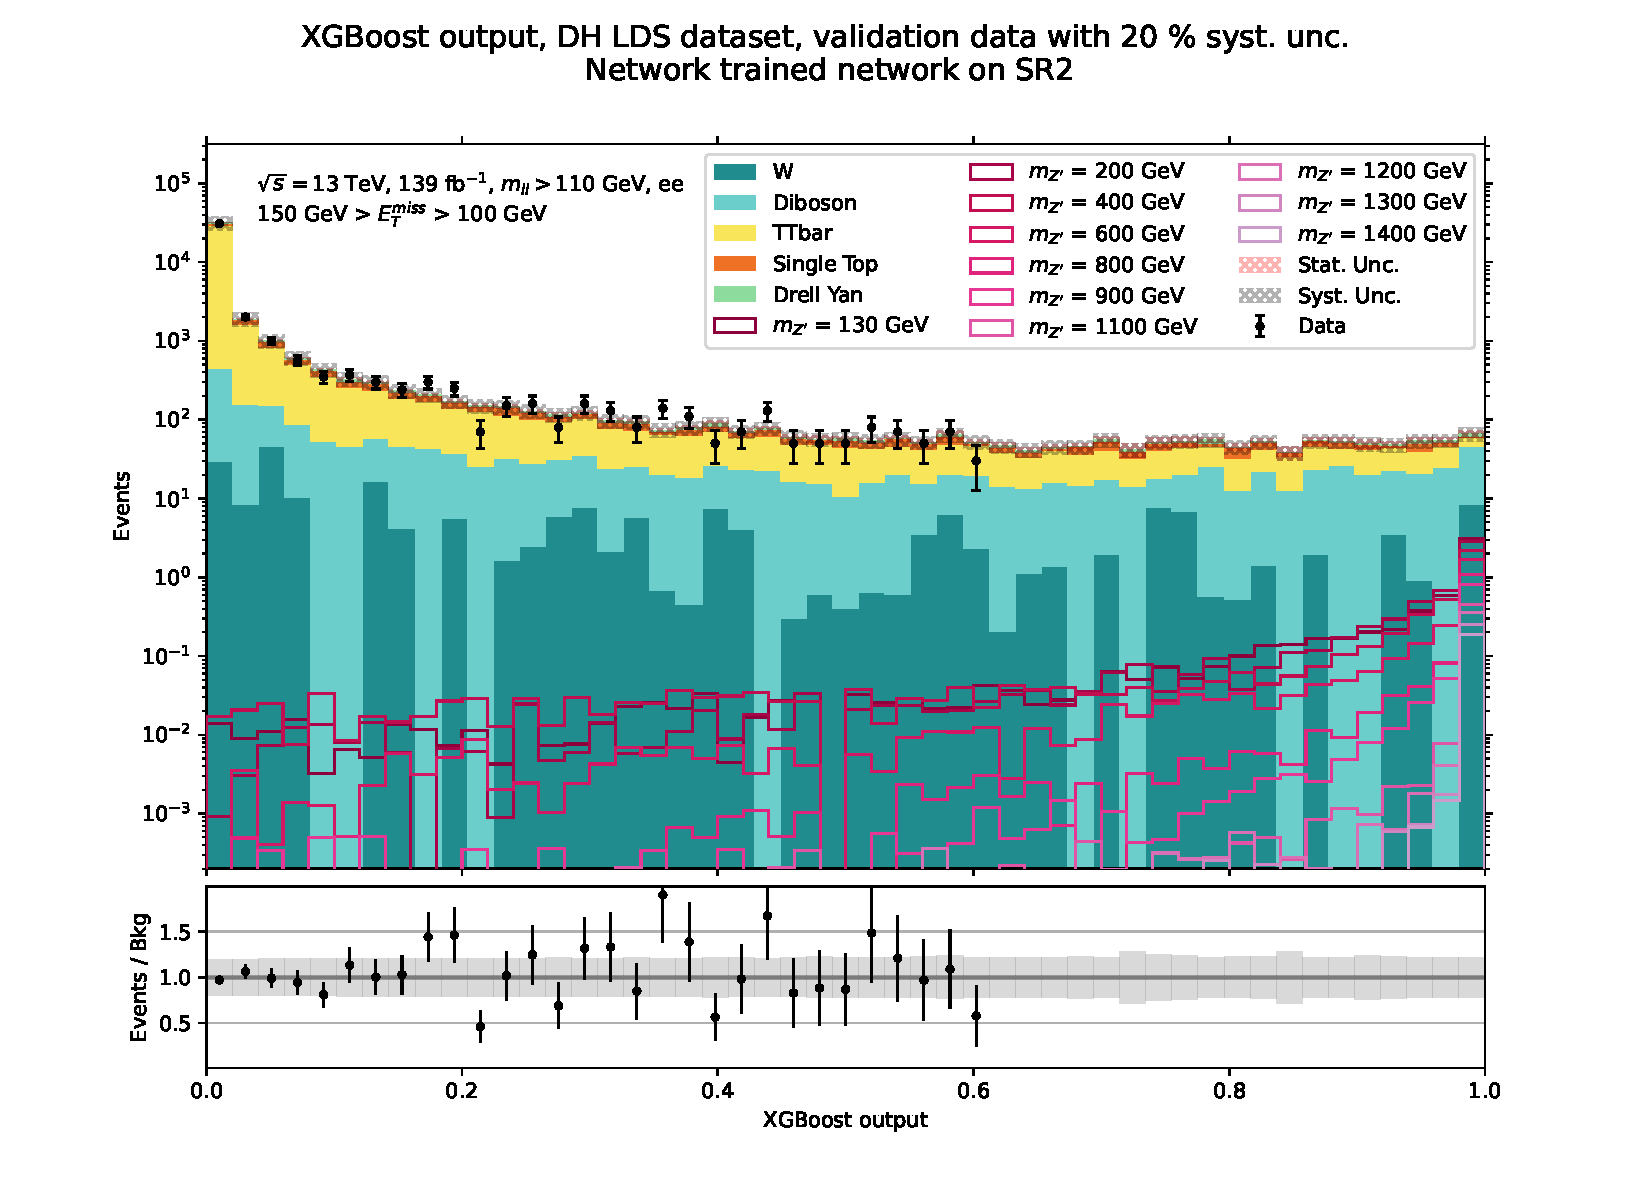
\includegraphics[width=1\textwidth]{XGBoost/Model_independent/100-150/DH_LDS/VAL_ee.pdf}
   \end{subfigure}
   \hfill
   \begin{subfigure}[b]{0.49\textwidth}
      \centering
      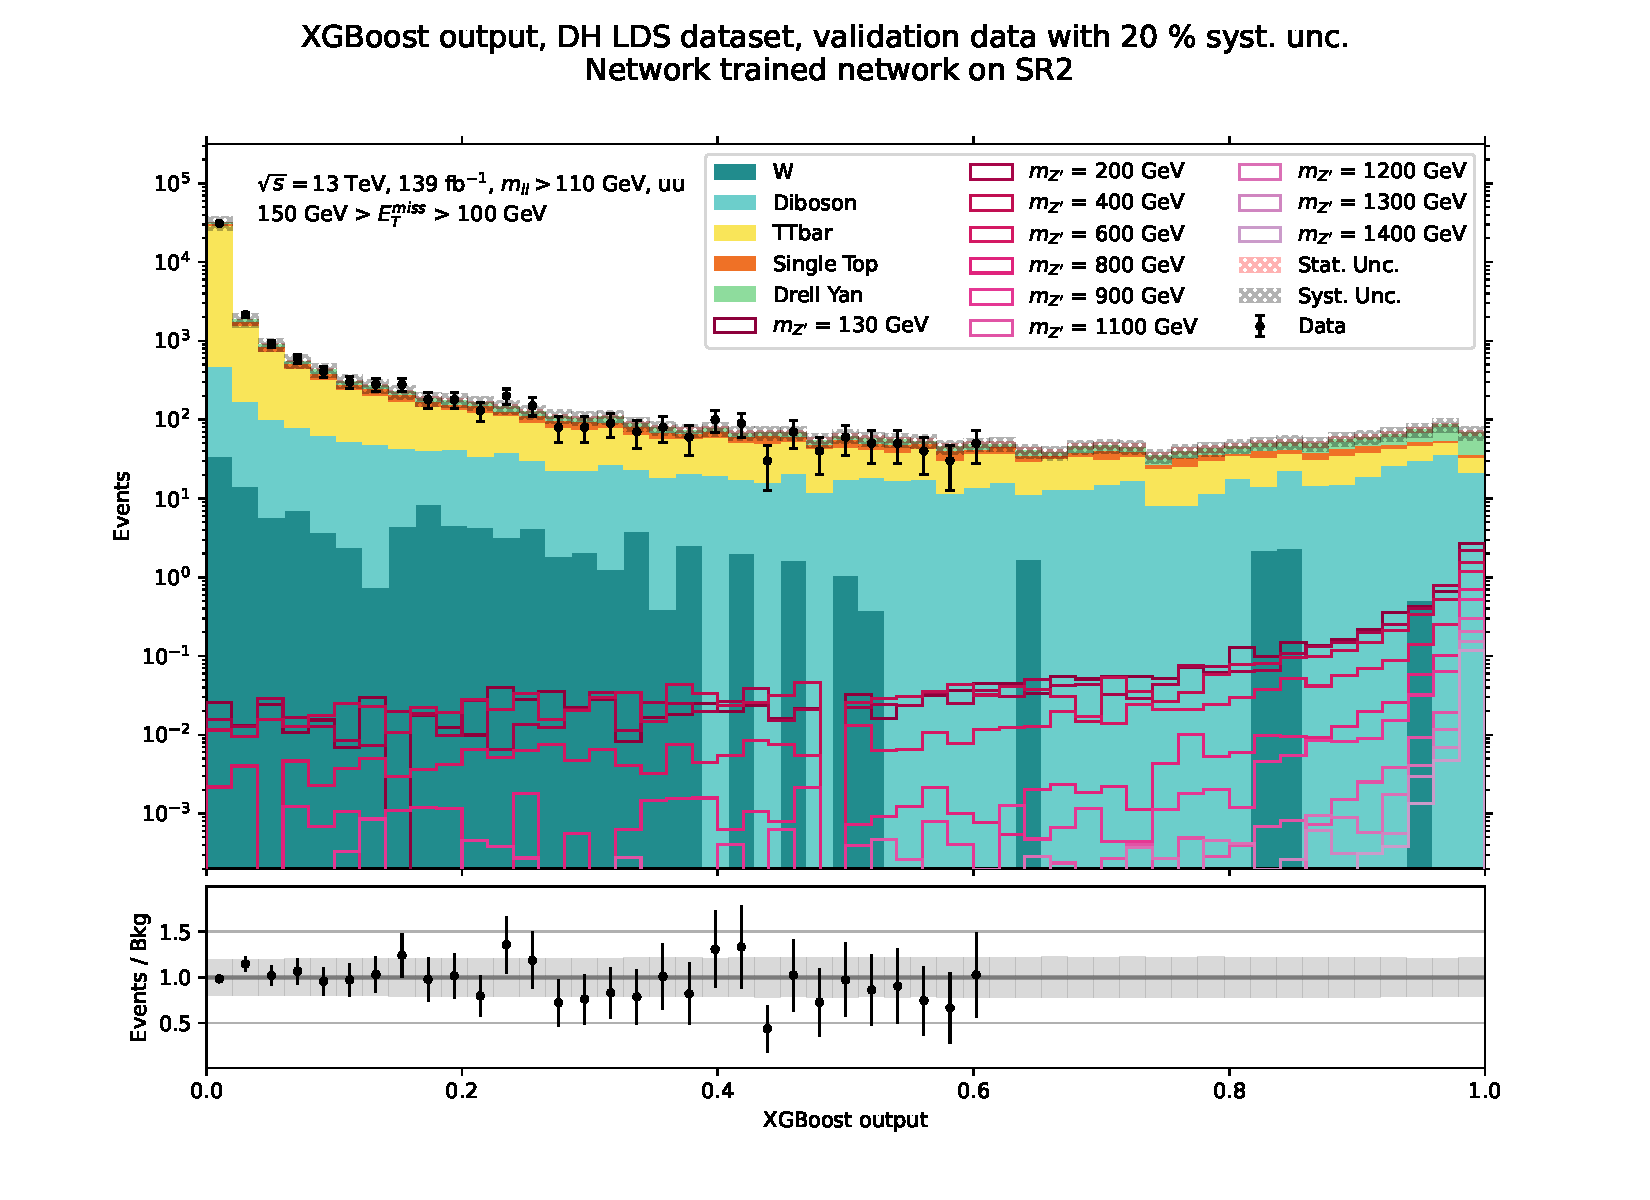
\includegraphics[width=1\textwidth]{XGBoost/Model_independent/100-150/DH_LDS/VAL_uu.pdf}
   \end{subfigure}
   \hfill
   \begin{subfigure}[b]{0.49\textwidth}
      \centering
      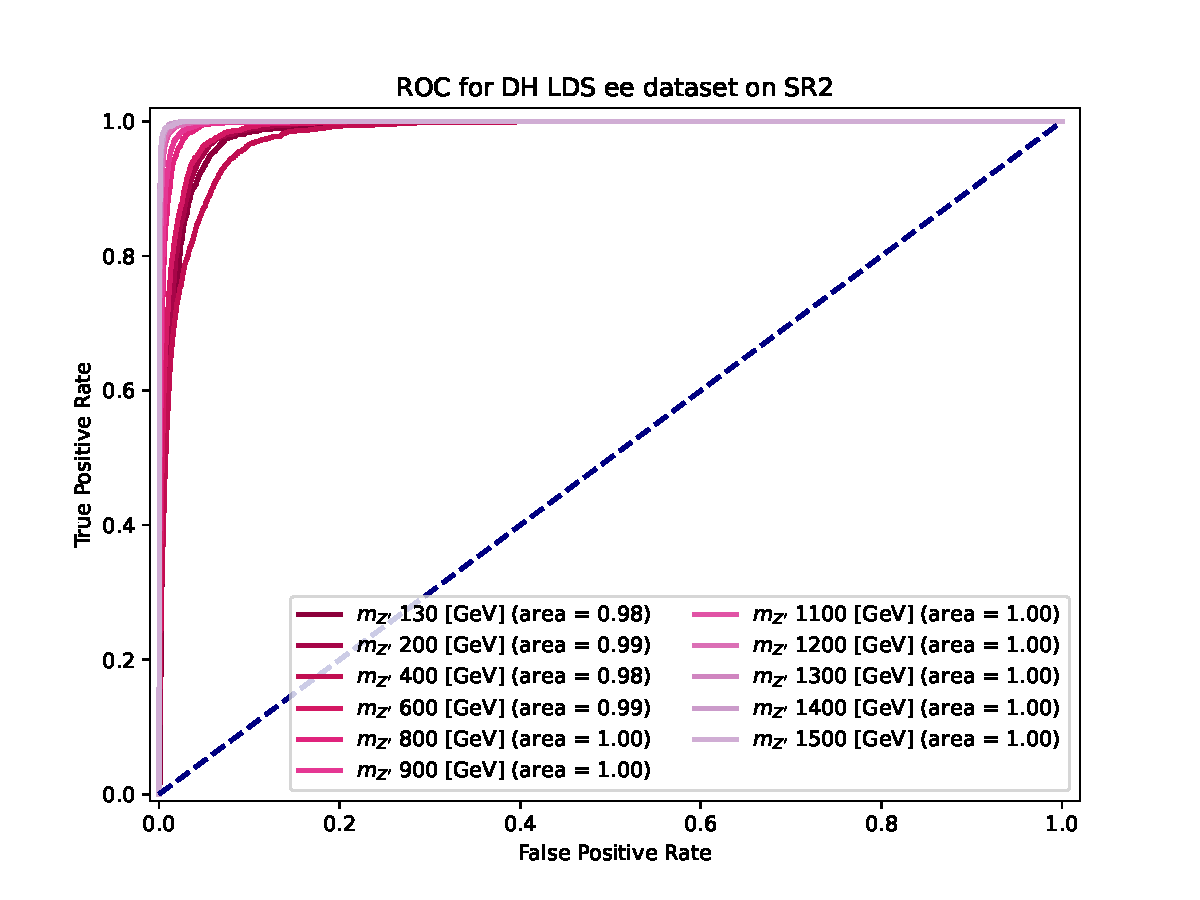
\includegraphics[width=1\textwidth]{XGBoost/Model_independent/100-150/DH_LDS/ROC_ee.pdf}
   \end{subfigure}
   \hfill
   \begin{subfigure}[b]{0.49\textwidth}
      \centering
      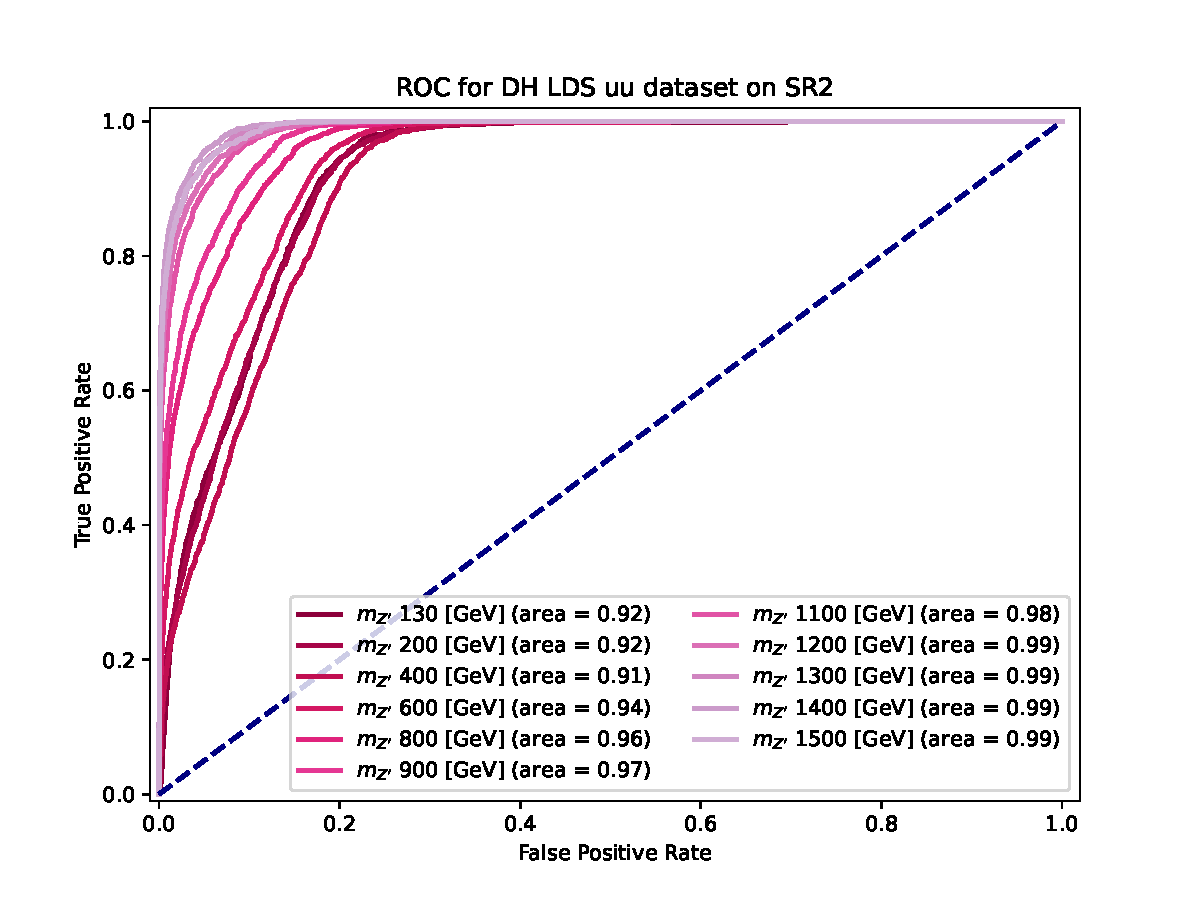
\includegraphics[width=1\textwidth]{XGBoost/Model_independent/100-150/DH_LDS/ROC_uu.pdf}
   \end{subfigure}
   \hfill
	\begin{subfigure}[b]{0.49\textwidth}
      \centering
      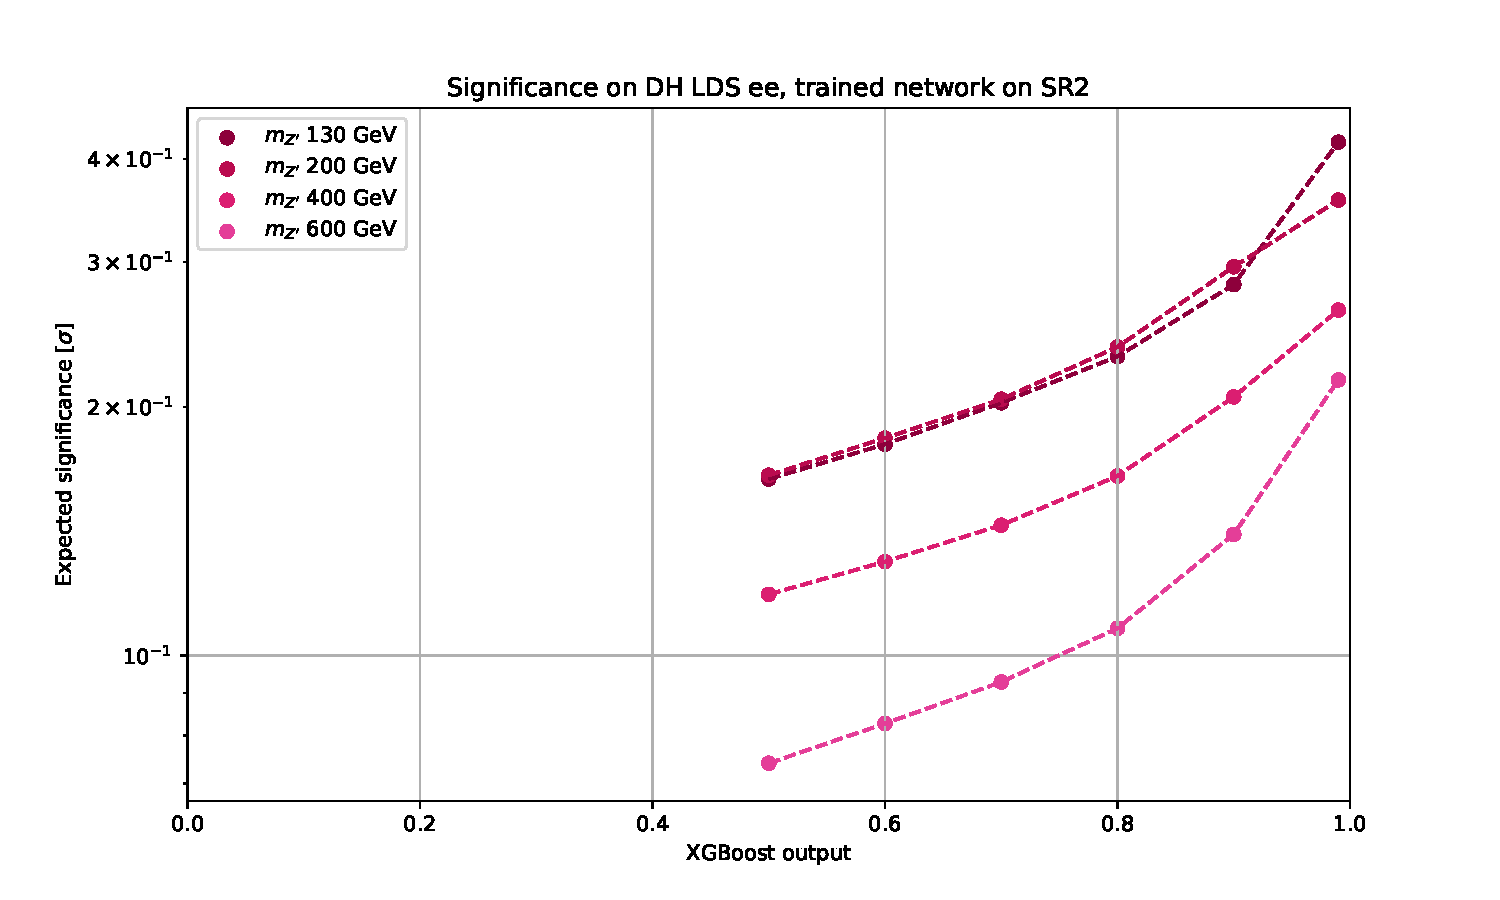
\includegraphics[width=1\textwidth]{XGBoost/Model_independent/100-150/DH_LDS/EXP_SIG_ee.pdf}
   \end{subfigure}
   \hfill
   \begin{subfigure}[b]{0.49\textwidth}
      \centering
      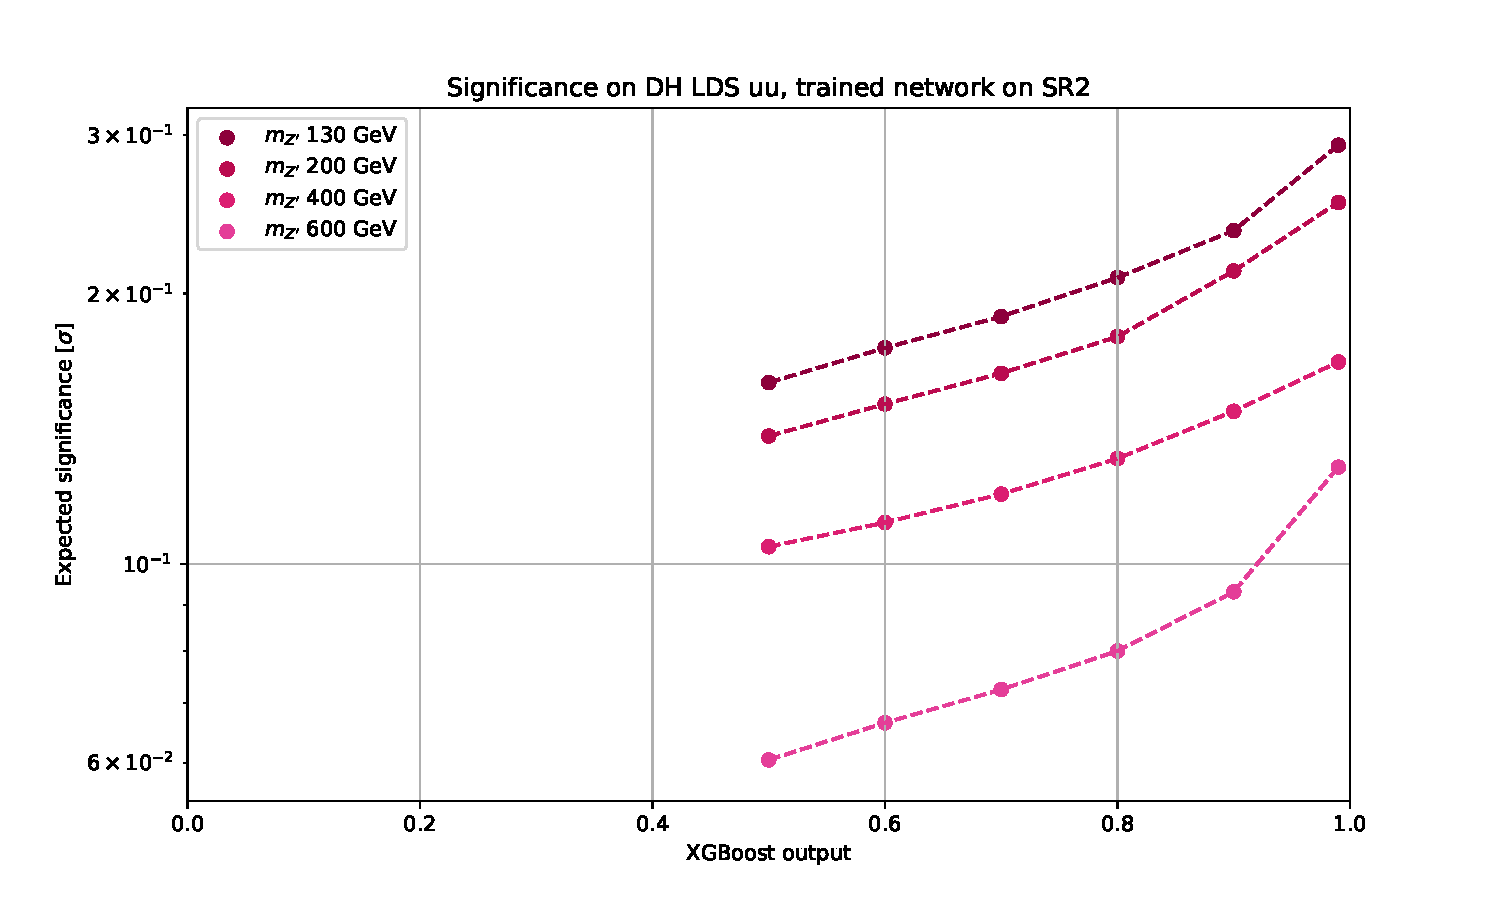
\includegraphics[width=1\textwidth]{XGBoost/Model_independent/100-150/DH_LDS/EXP_SIG_uu.pdf}
   \end{subfigure}
   \caption{XGBoost results for DH LDS model on $ee$ and $\mu\mu$ channel in SR2}\label{fig:DH_LDS_SR2}
\end{figure}

\begin{figure}[!ht]
	\centering
	\begin{subfigure}[b]{0.49\textwidth}
      \centering
      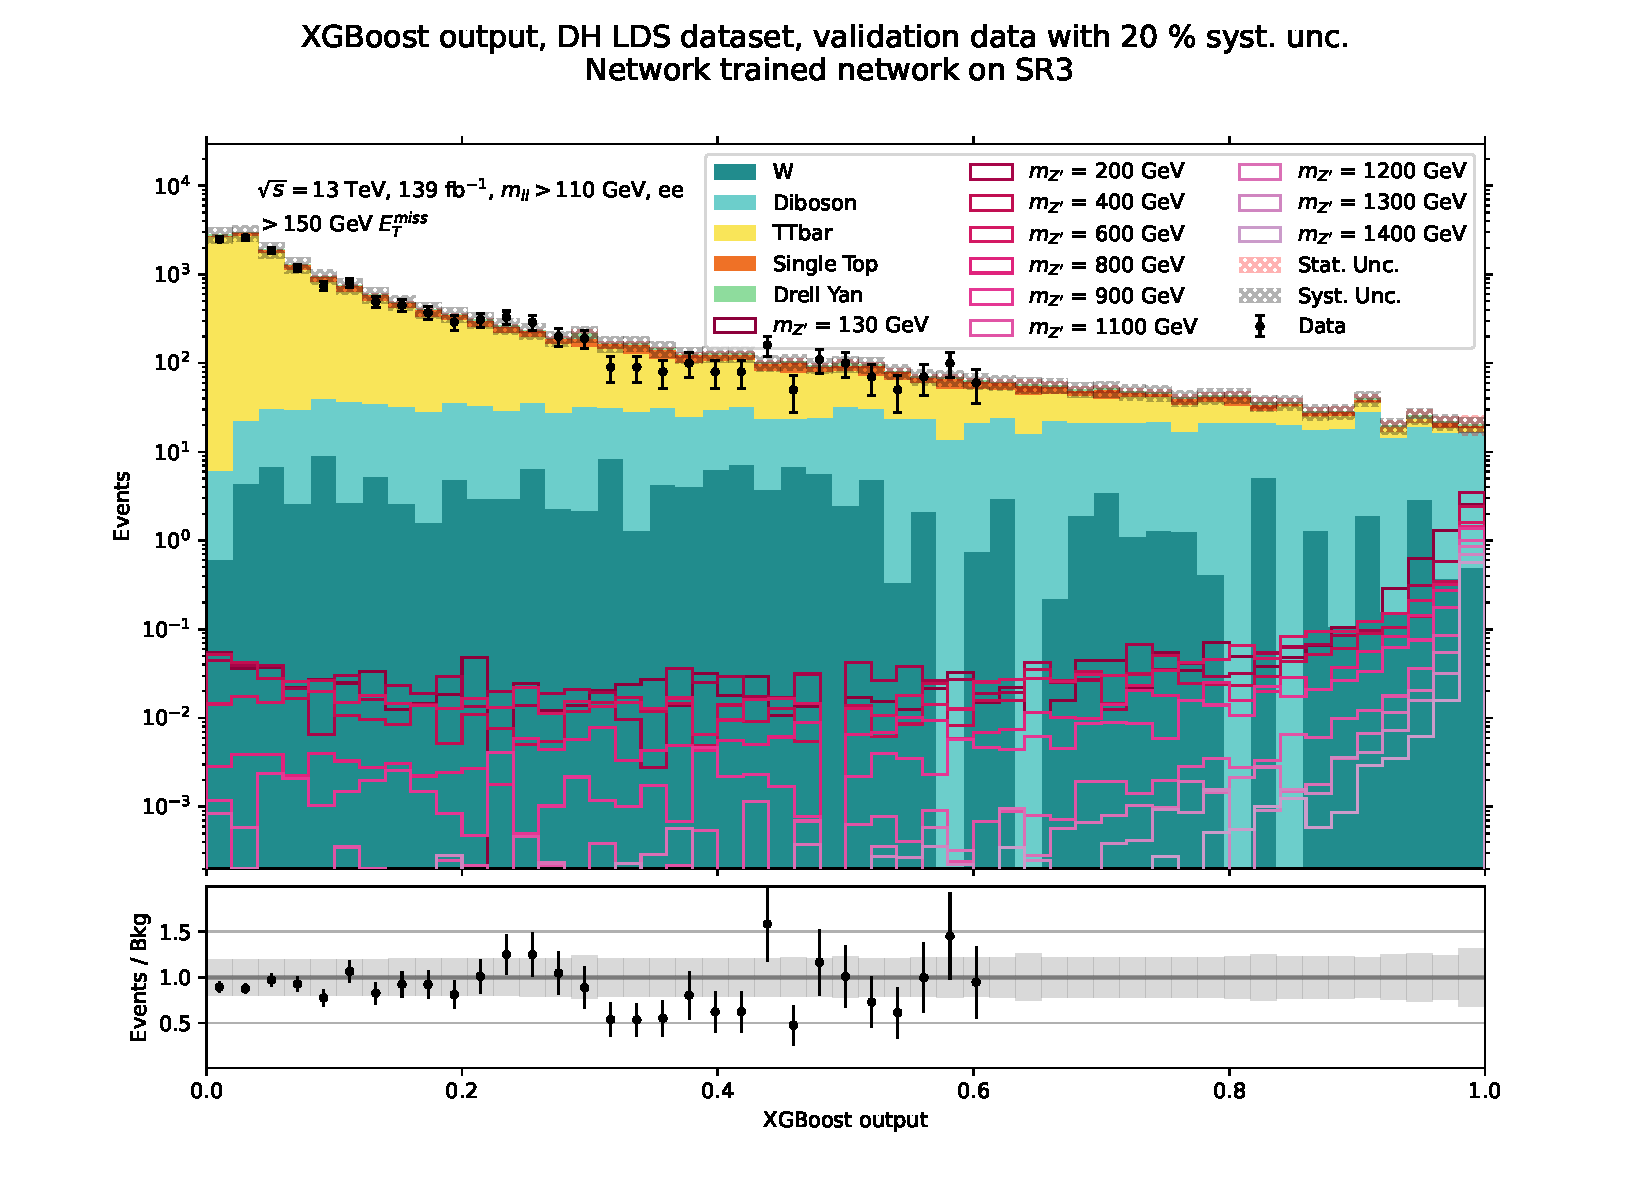
\includegraphics[width=1\textwidth]{XGBoost/Model_independent/150/DH_LDS/VAL_ee.pdf}
   \end{subfigure}
   \hfill
   \begin{subfigure}[b]{0.49\textwidth}
      \centering
      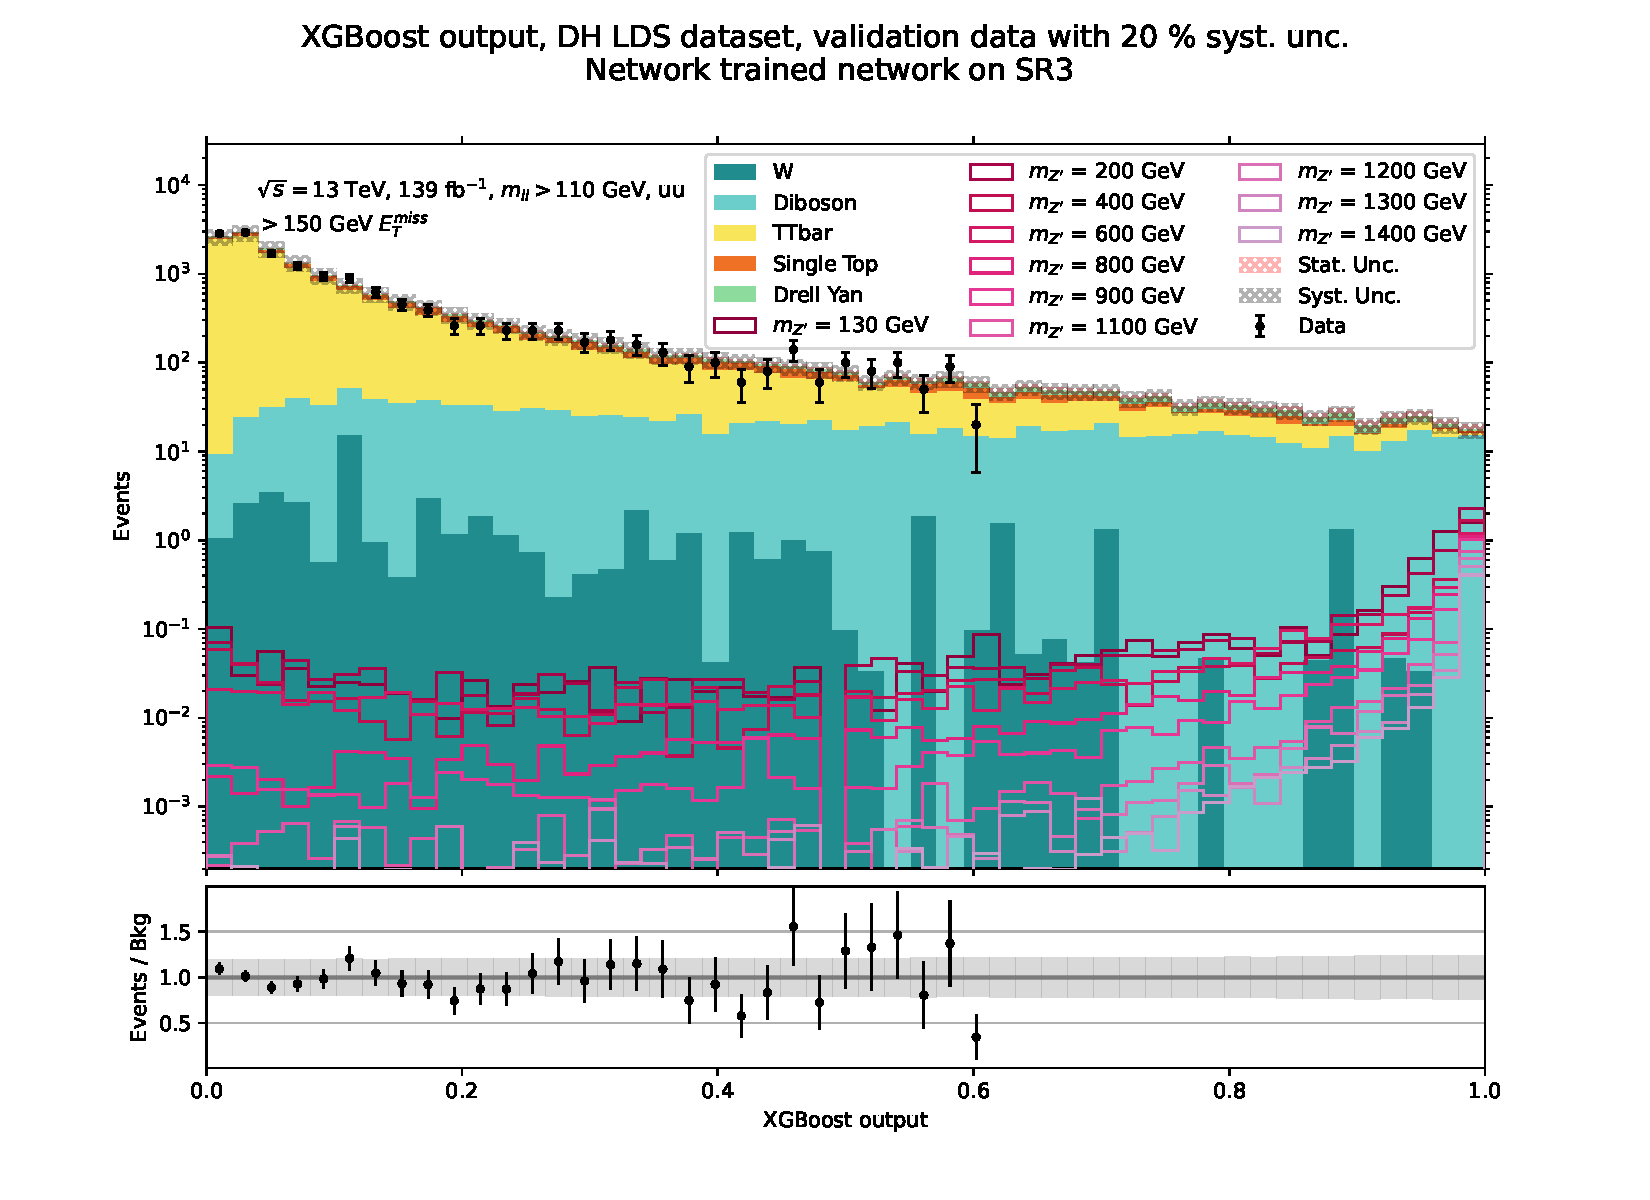
\includegraphics[width=1\textwidth]{XGBoost/Model_independent/150/DH_LDS/VAL_uu.pdf}
   \end{subfigure}
   \hfill
   \begin{subfigure}[b]{0.49\textwidth}
      \centering
      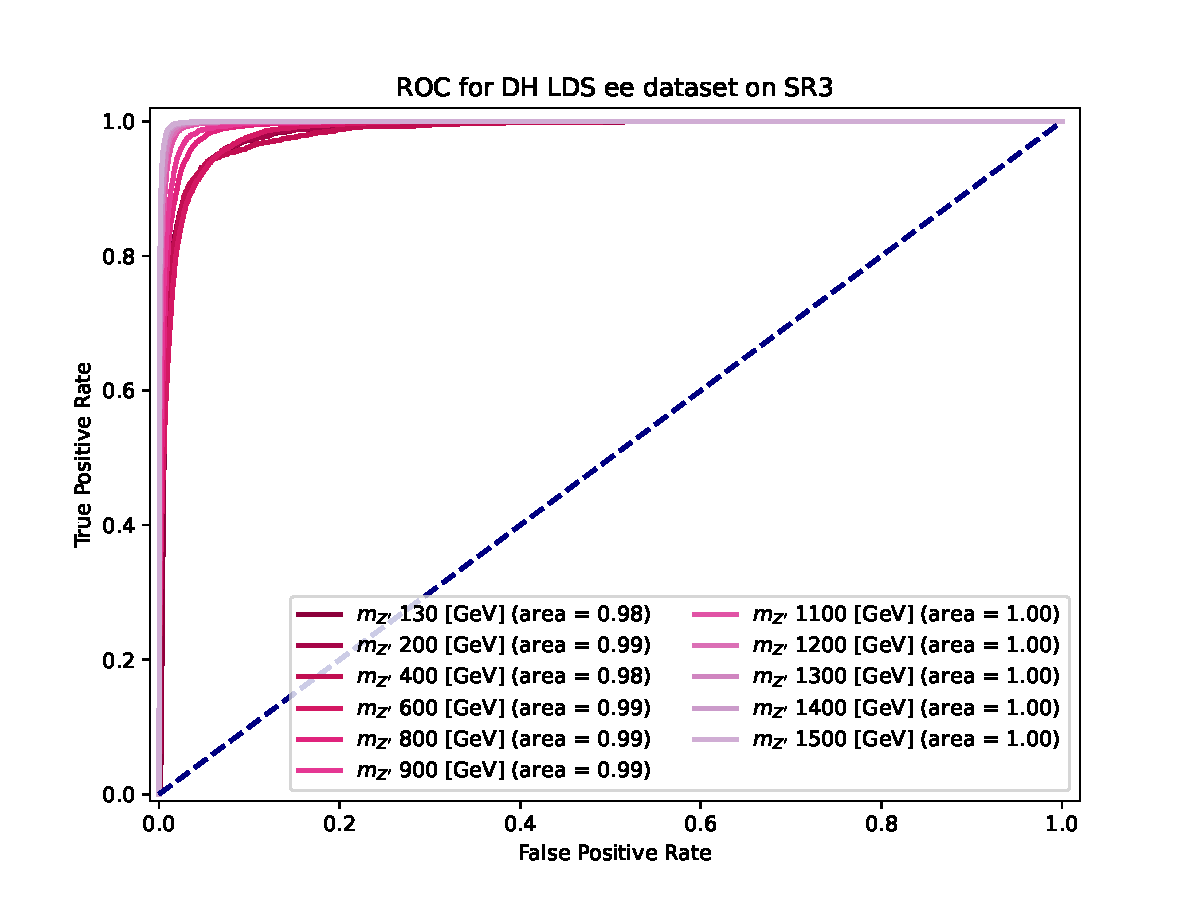
\includegraphics[width=1\textwidth]{XGBoost/Model_independent/150/DH_LDS/ROC_ee.pdf}
   \end{subfigure}
   \hfill
   \begin{subfigure}[b]{0.49\textwidth}
      \centering
      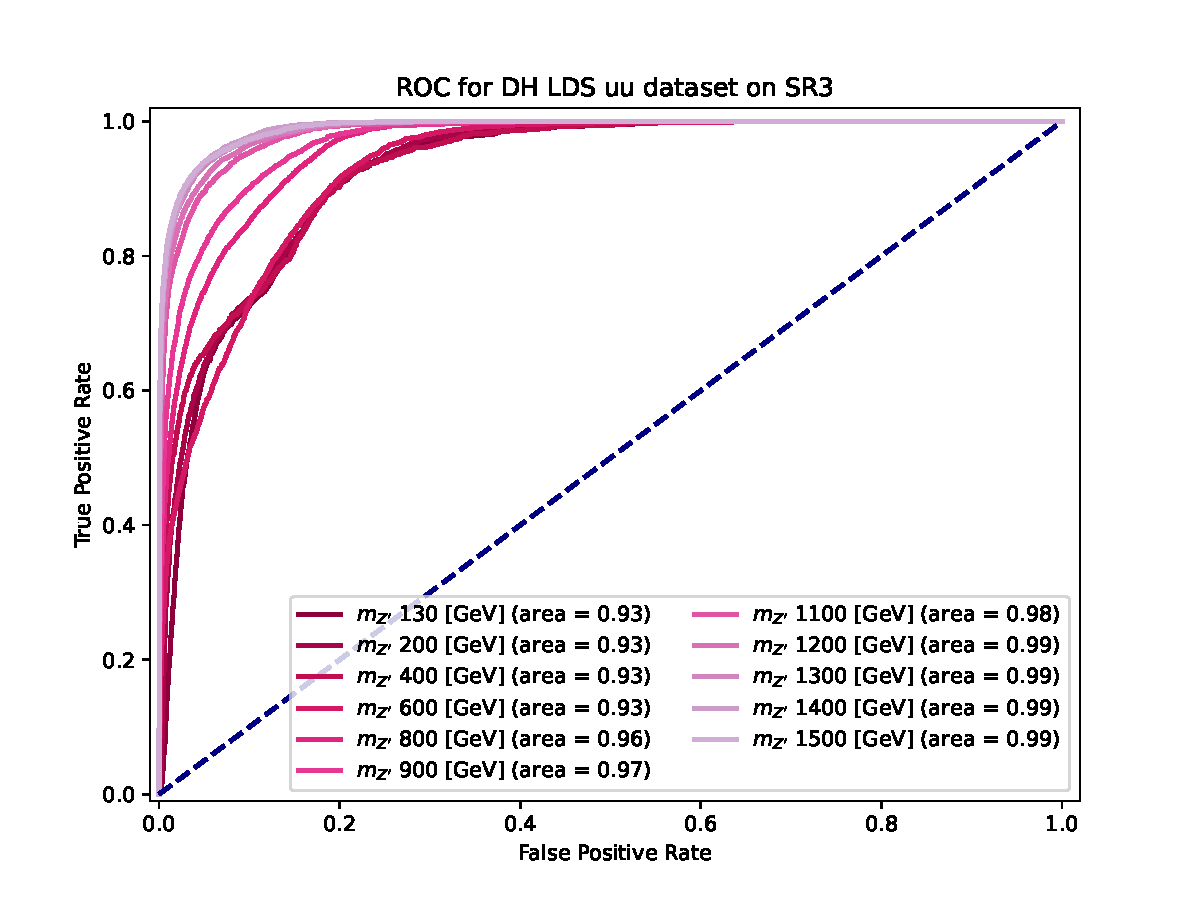
\includegraphics[width=1\textwidth]{XGBoost/Model_independent/150/DH_LDS/ROC_uu.pdf}
   \end{subfigure}
   \hfill
	\begin{subfigure}[b]{0.49\textwidth}
      \centering
      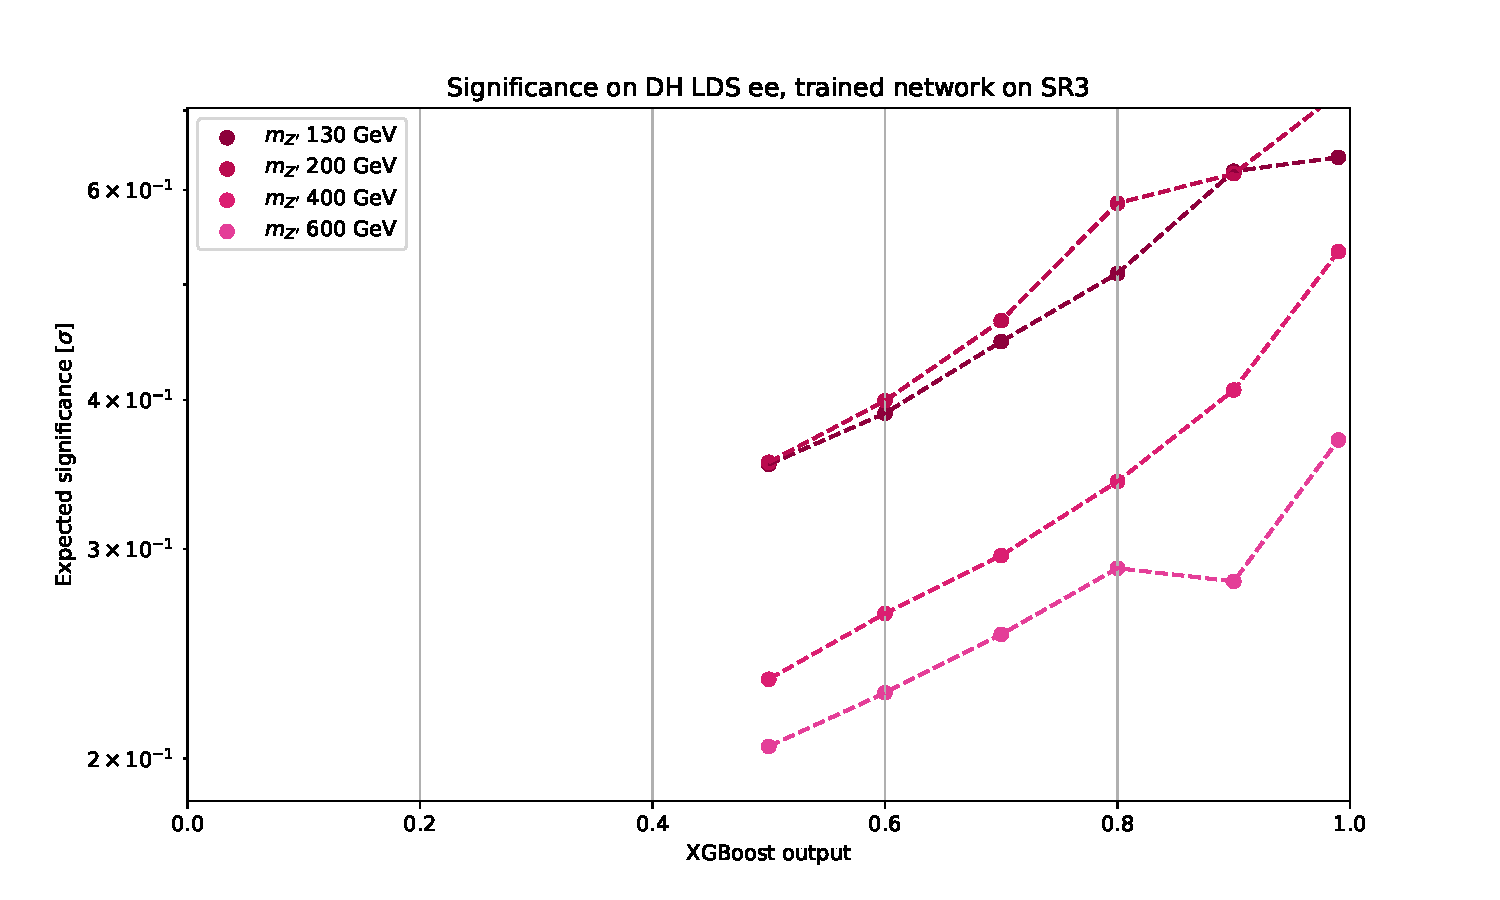
\includegraphics[width=1\textwidth]{XGBoost/Model_independent/150/DH_LDS/EXP_SIG_ee.pdf}
   \end{subfigure}
   \hfill
   \begin{subfigure}[b]{0.49\textwidth}
      \centering
      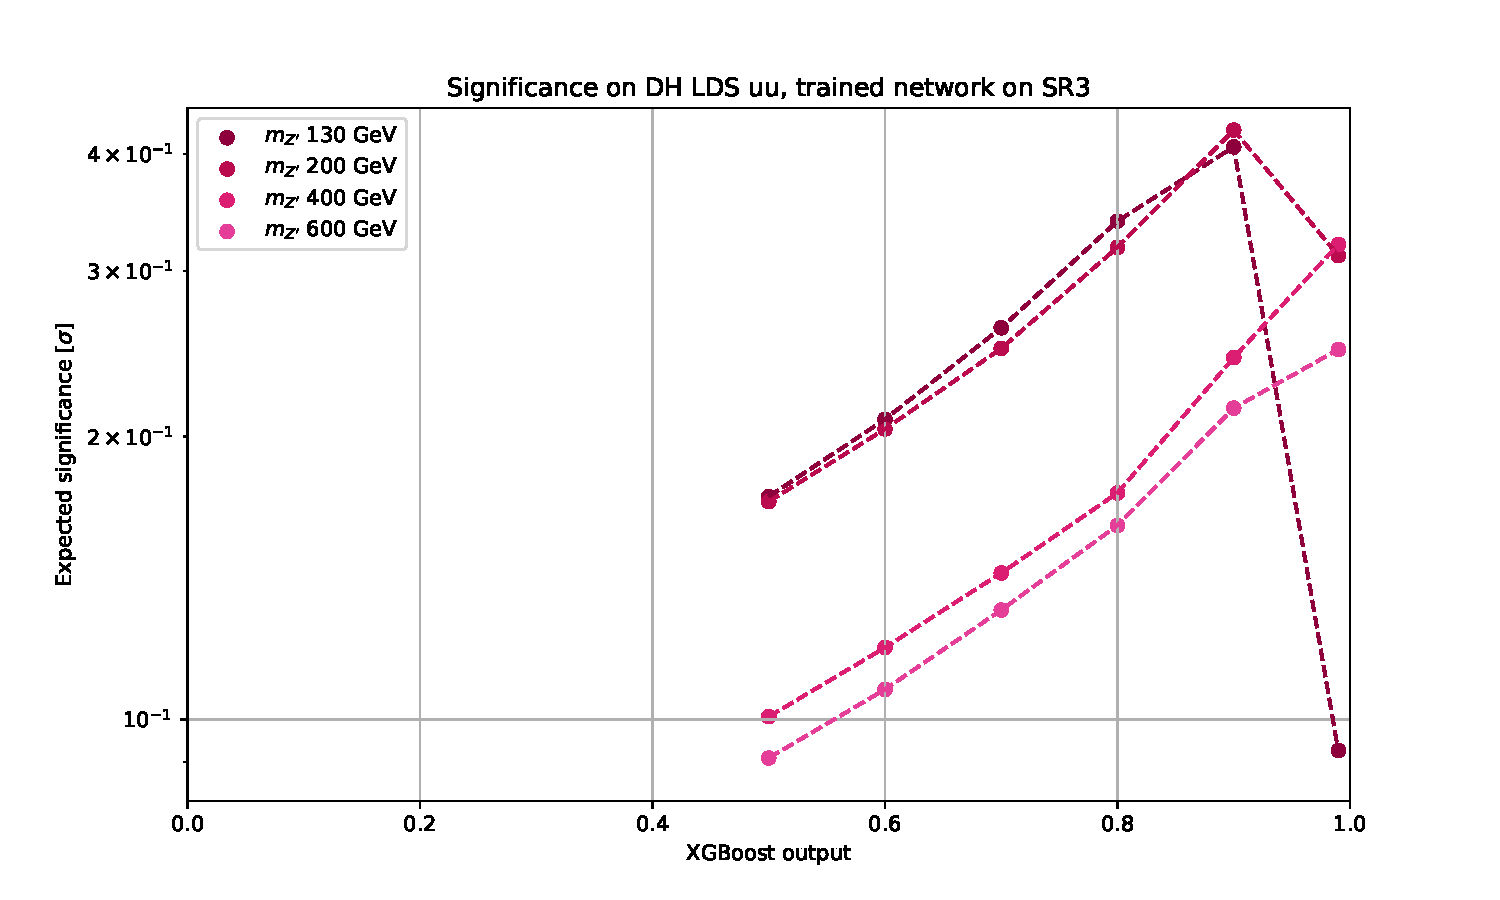
\includegraphics[width=1\textwidth]{XGBoost/Model_independent/150/DH_LDS/EXP_SIG_uu.pdf}
   \end{subfigure}
   \caption{XGBoost results for DH LDS model on $ee$ and $\mu\mu$ channel in SR3}\label{fig:DH_LDS_SR3}
\end{figure}

\begin{figure}[!ht]
	\centering
	\begin{subfigure}[b]{0.49\textwidth}
      \centering
      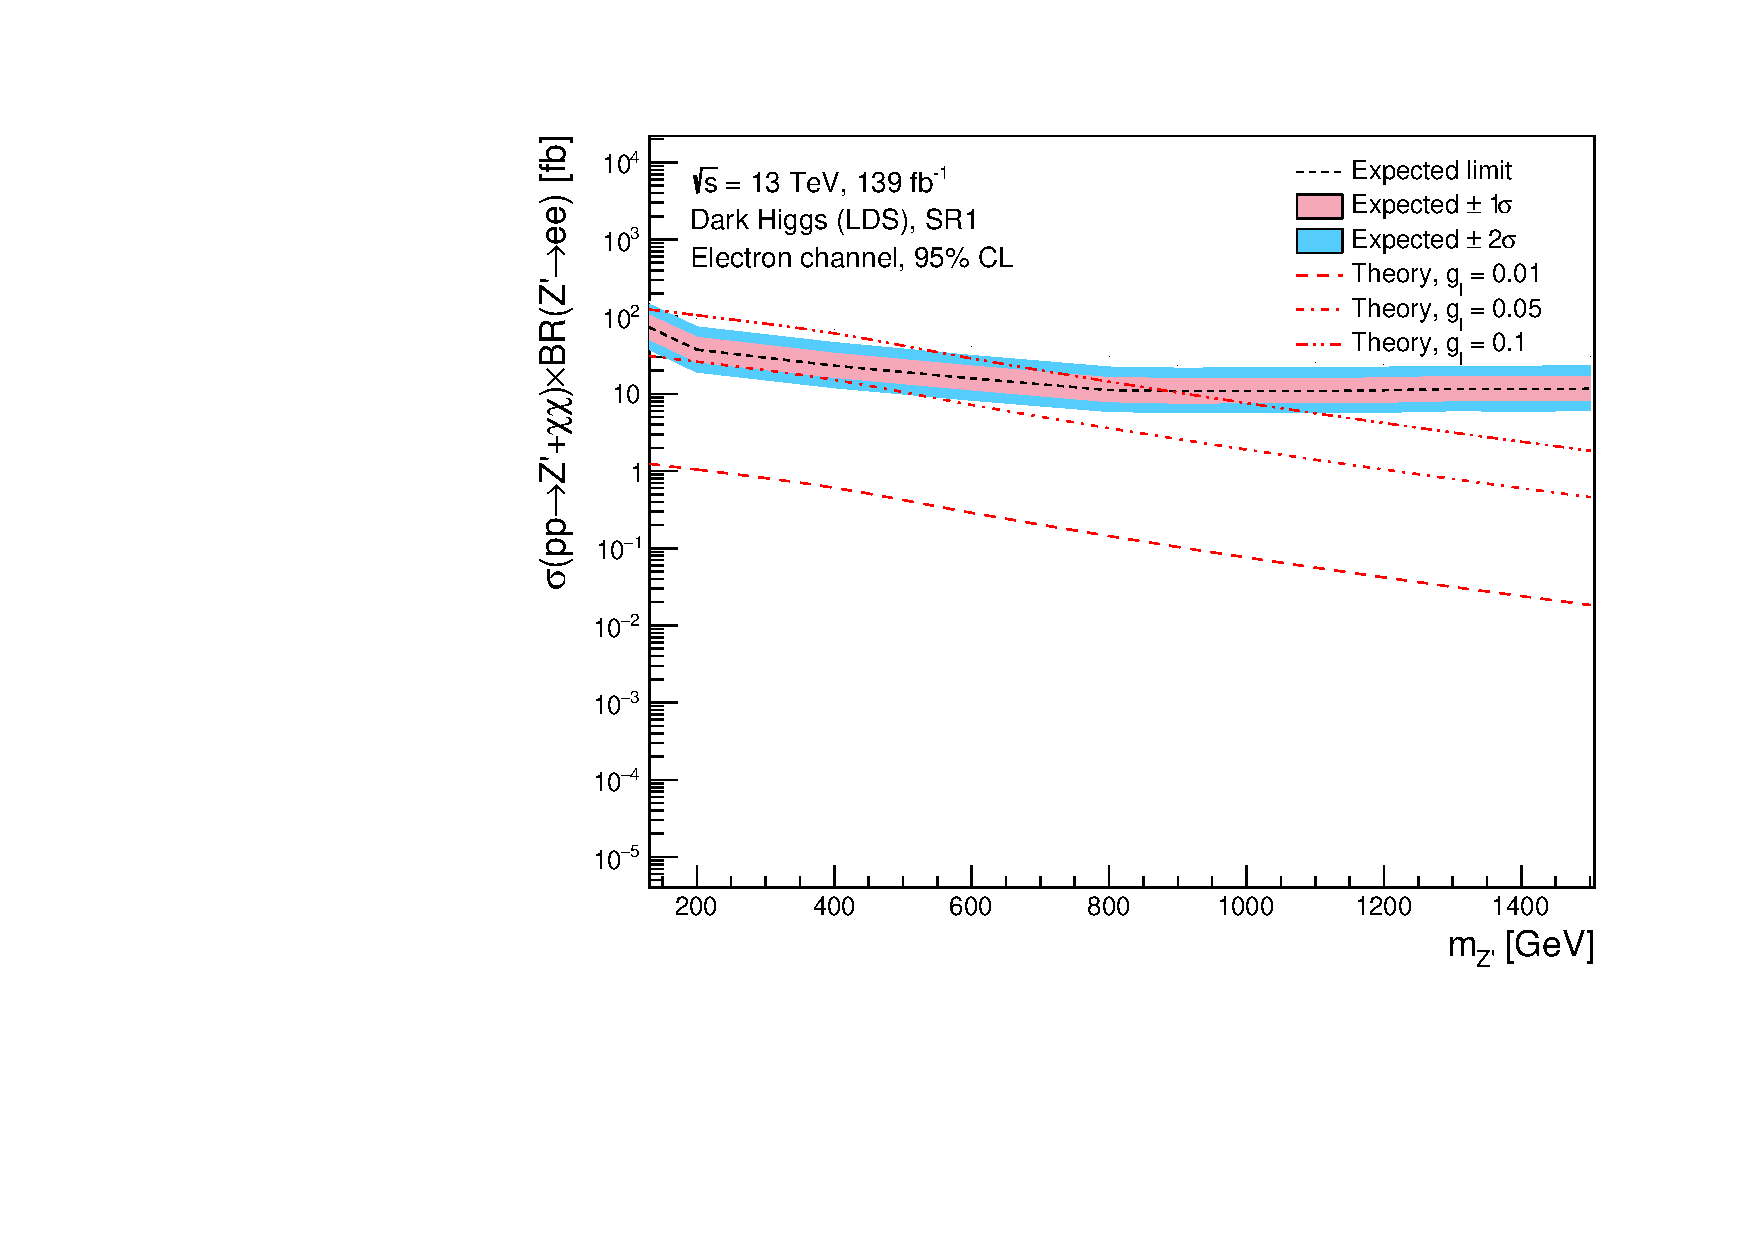
\includegraphics[width=1\textwidth]{Limits/Model_independent/50-100/DH_LDS/mass_exclusion_ee.pdf}
   \end{subfigure}
   \hfill
   \begin{subfigure}[b]{0.49\textwidth}
      \centering
      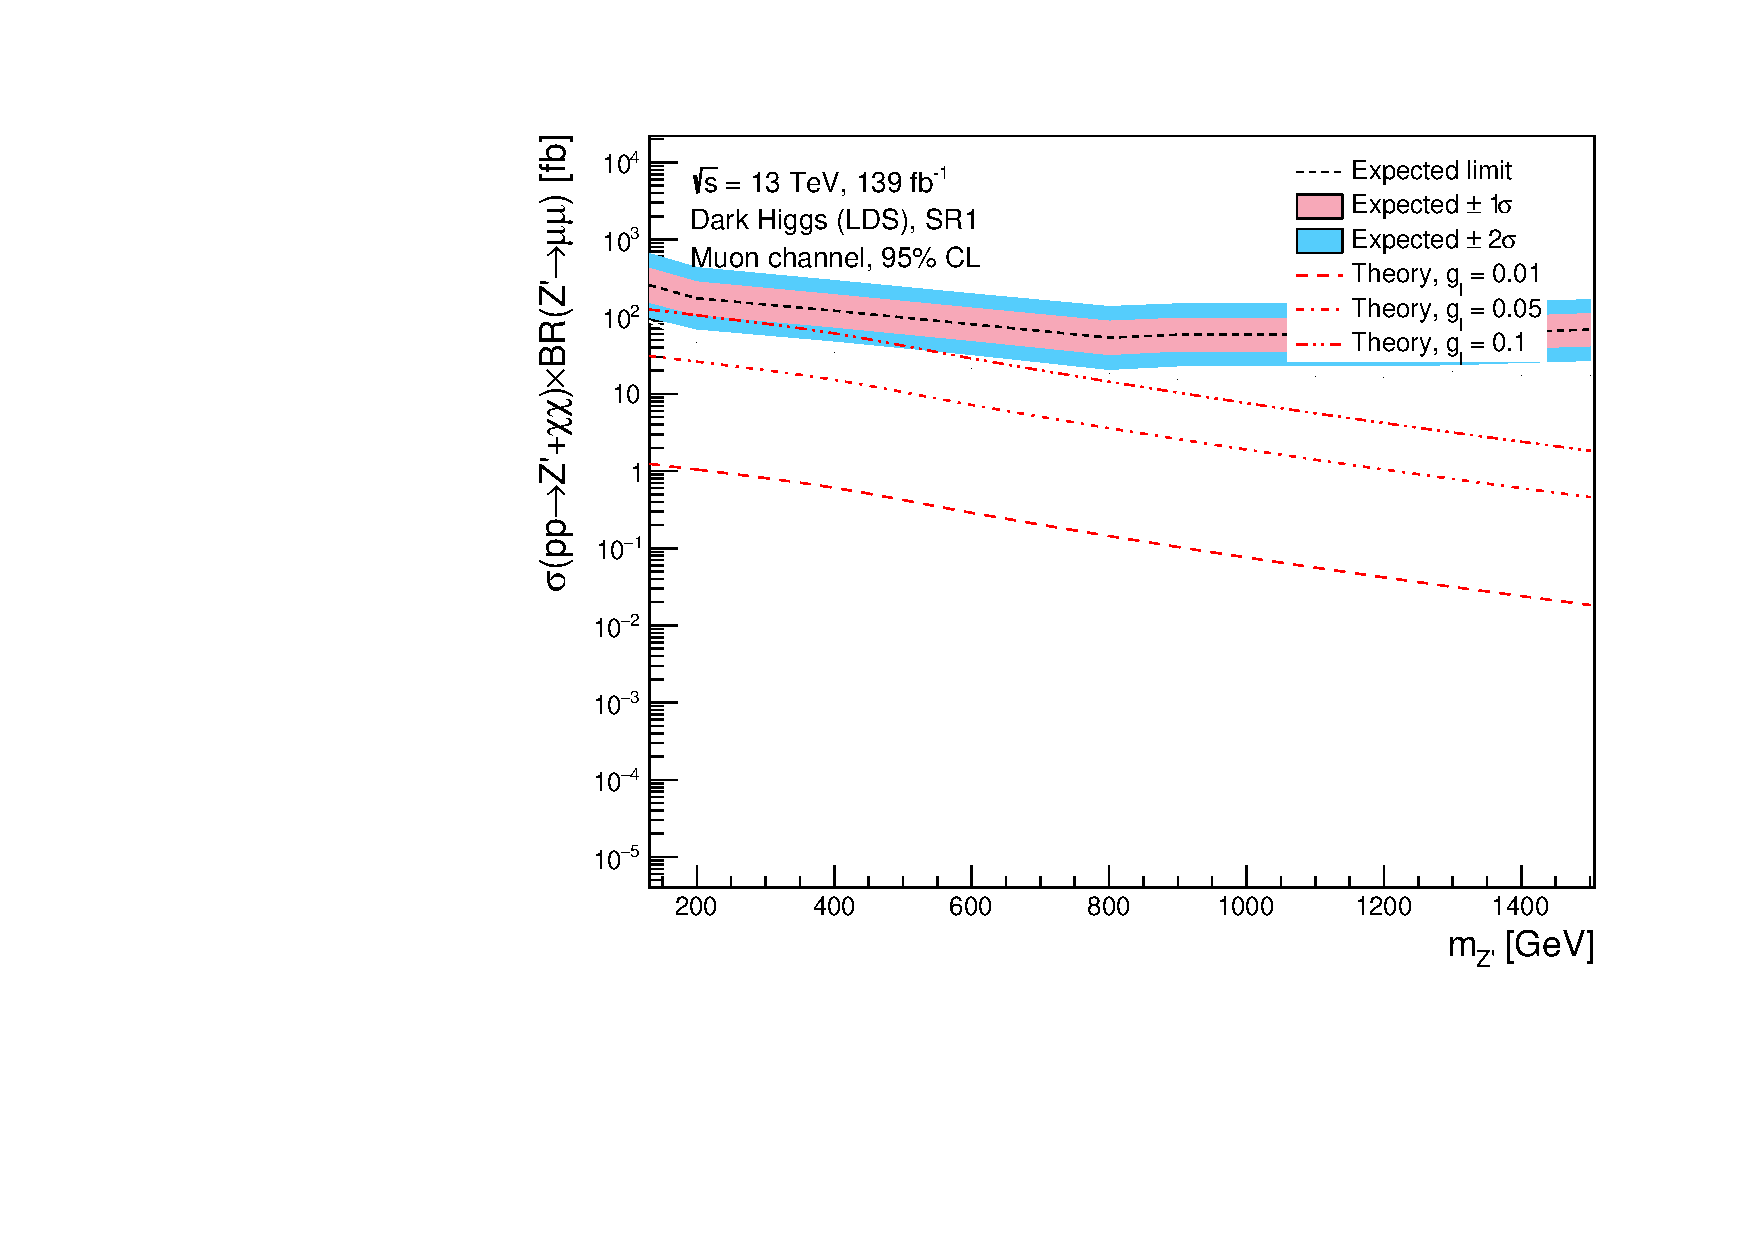
\includegraphics[width=1\textwidth]{Limits/Model_independent/50-100/DH_LDS/mass_exclusion_uu.pdf}
   \end{subfigure}
   \hfill
   \begin{subfigure}[b]{0.49\textwidth}
      \centering
      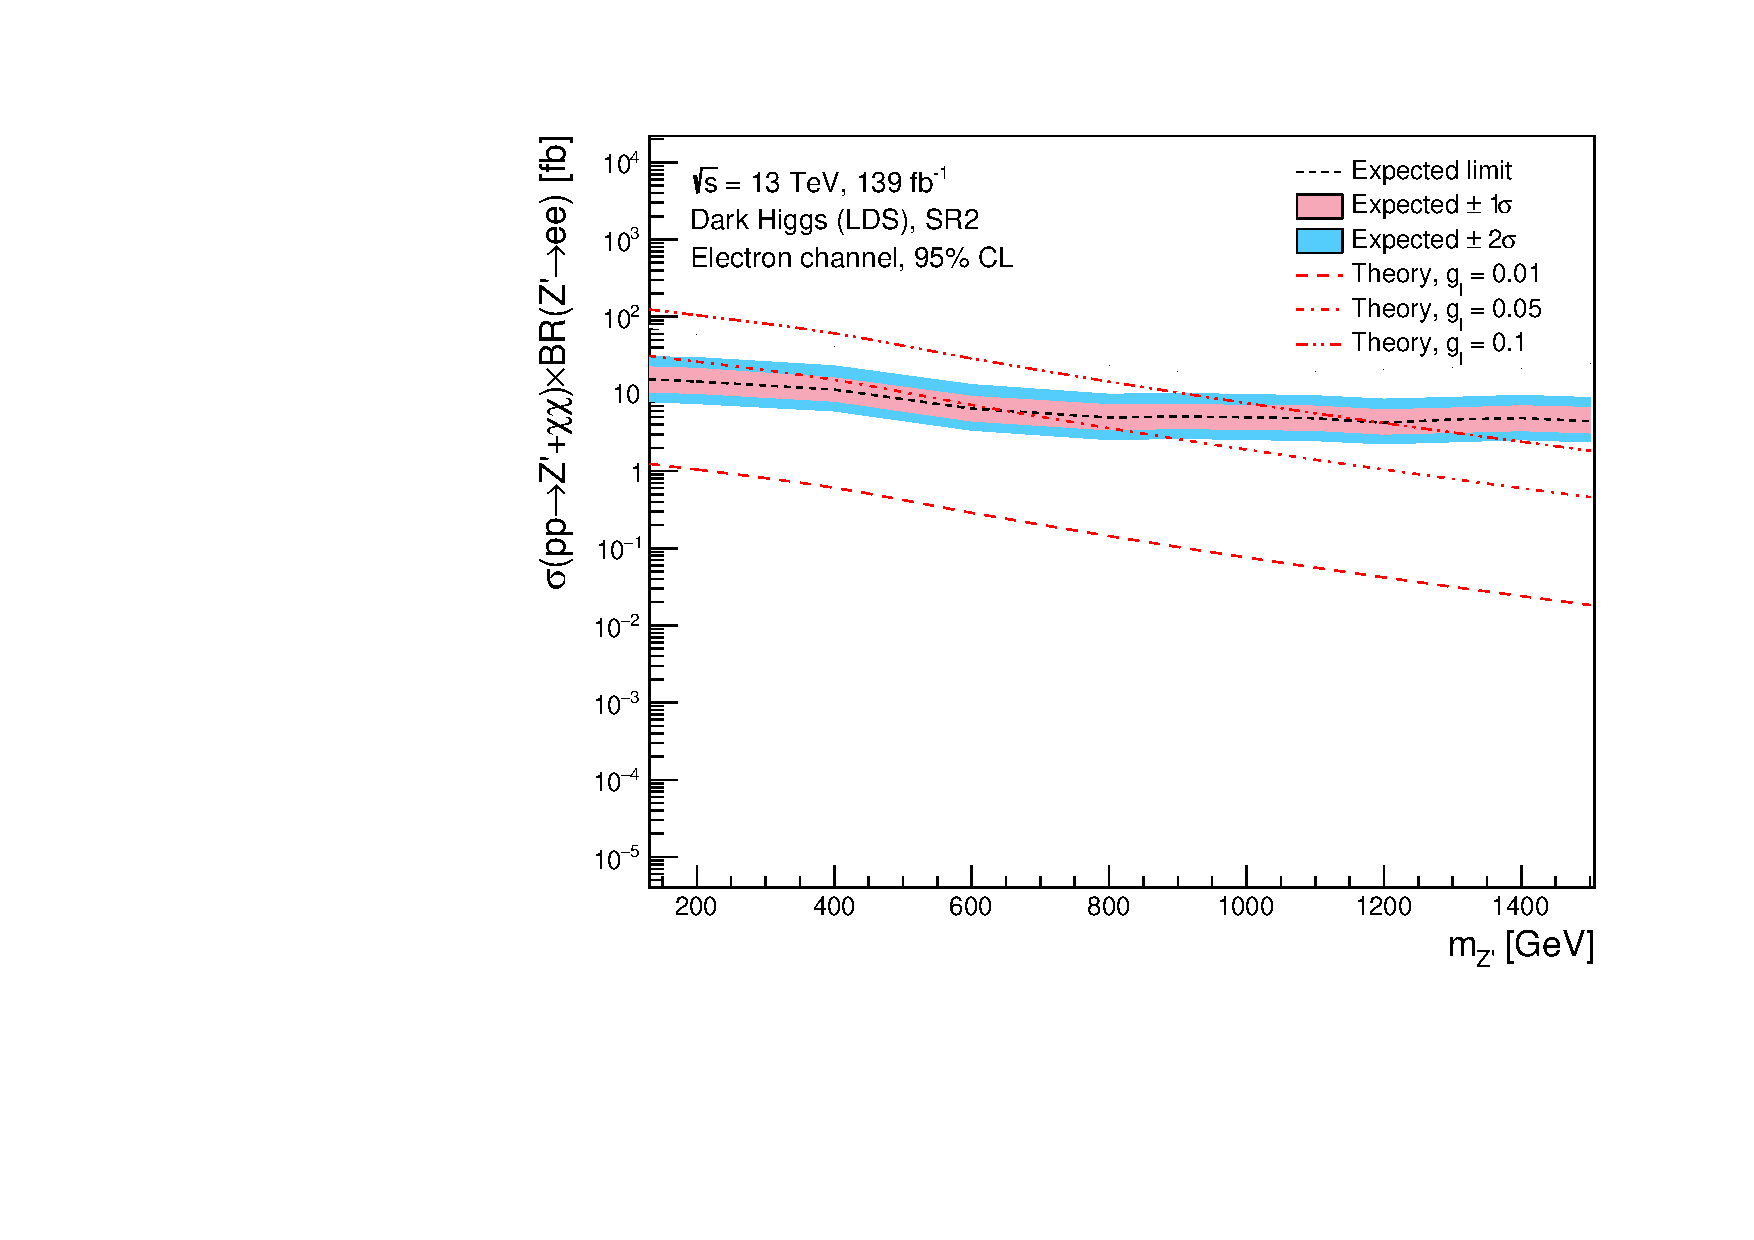
\includegraphics[width=1\textwidth]{Limits/Model_independent/100-150/DH_LDS/mass_exclusion_ee.pdf}
   \end{subfigure}
   \hfill
   \begin{subfigure}[b]{0.49\textwidth}
      \centering
      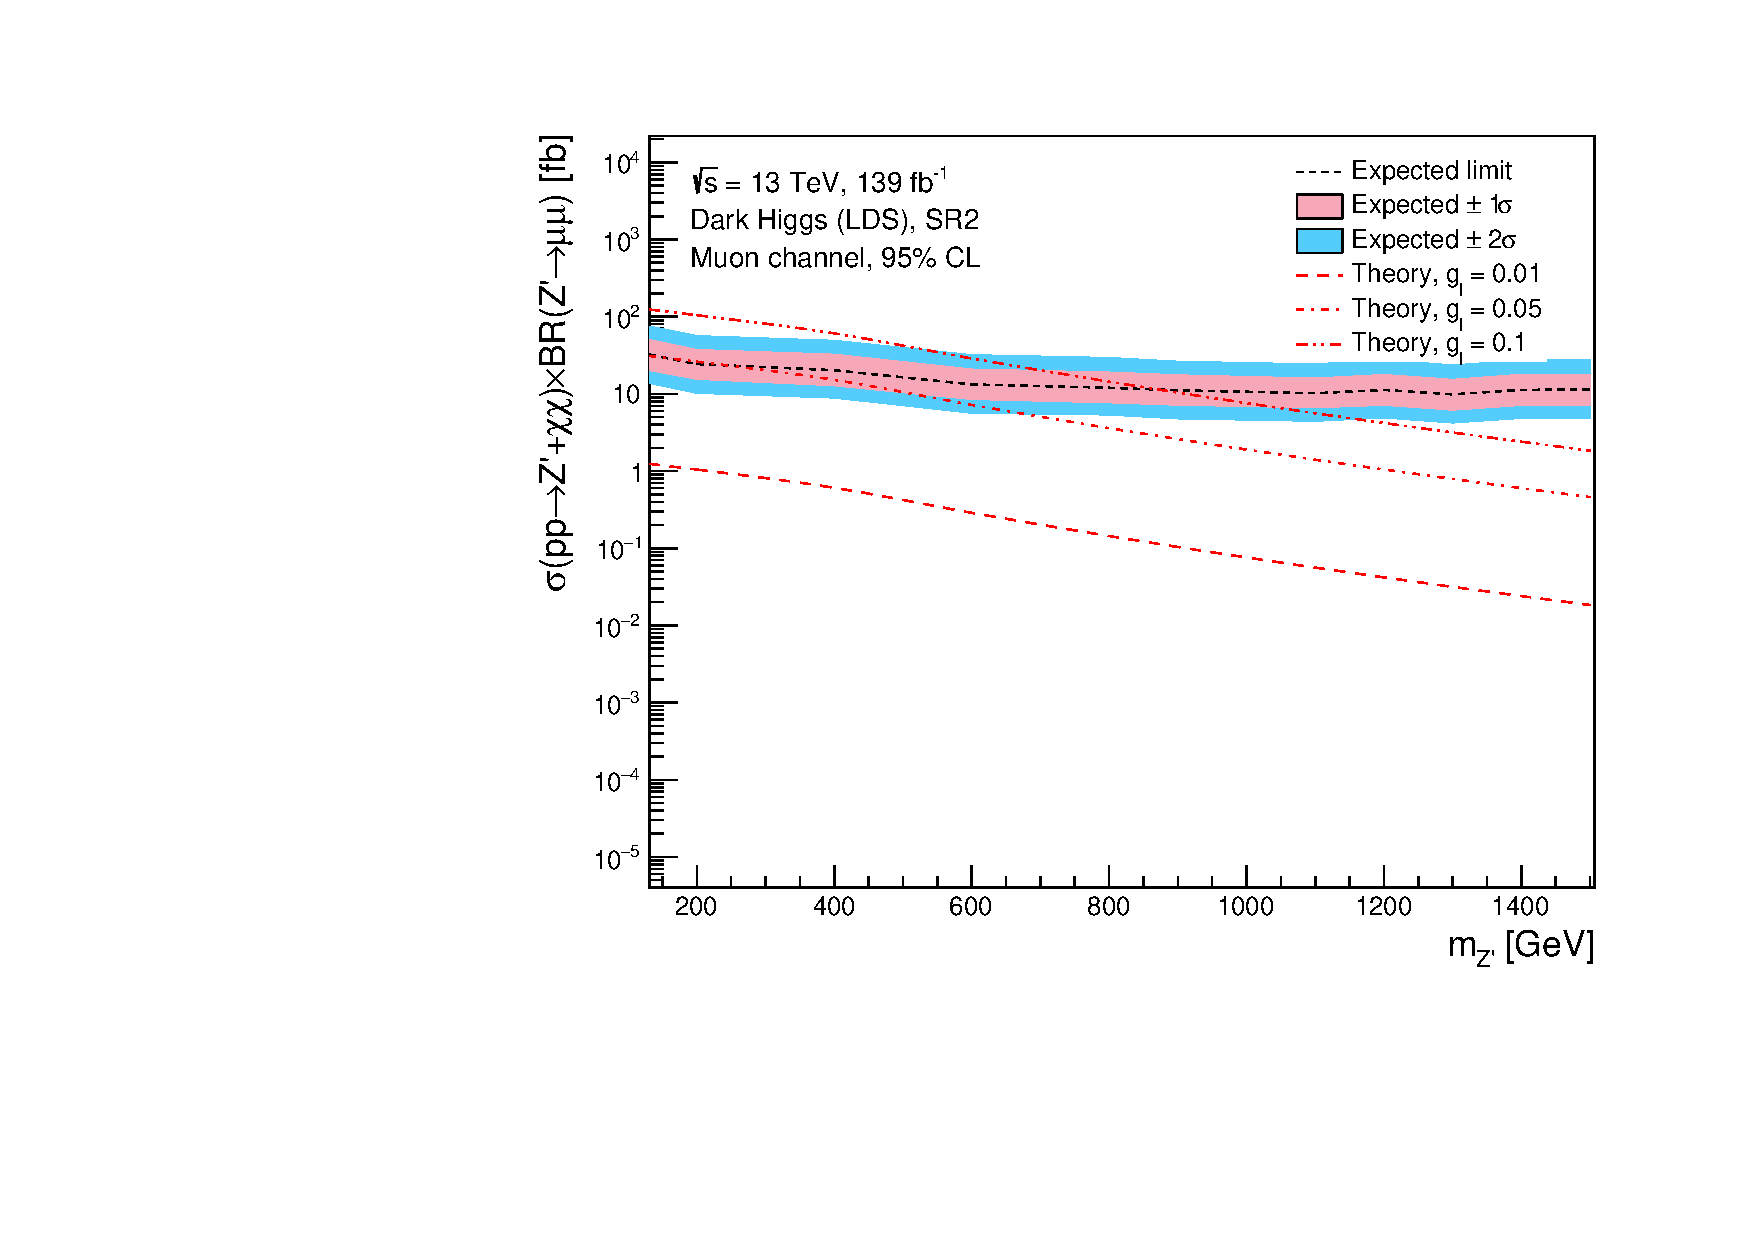
\includegraphics[width=1\textwidth]{Limits/Model_independent/100-150/DH_LDS/mass_exclusion_uu.pdf}
   \end{subfigure}
   \hfill
	\begin{subfigure}[b]{0.49\textwidth}
      \centering
      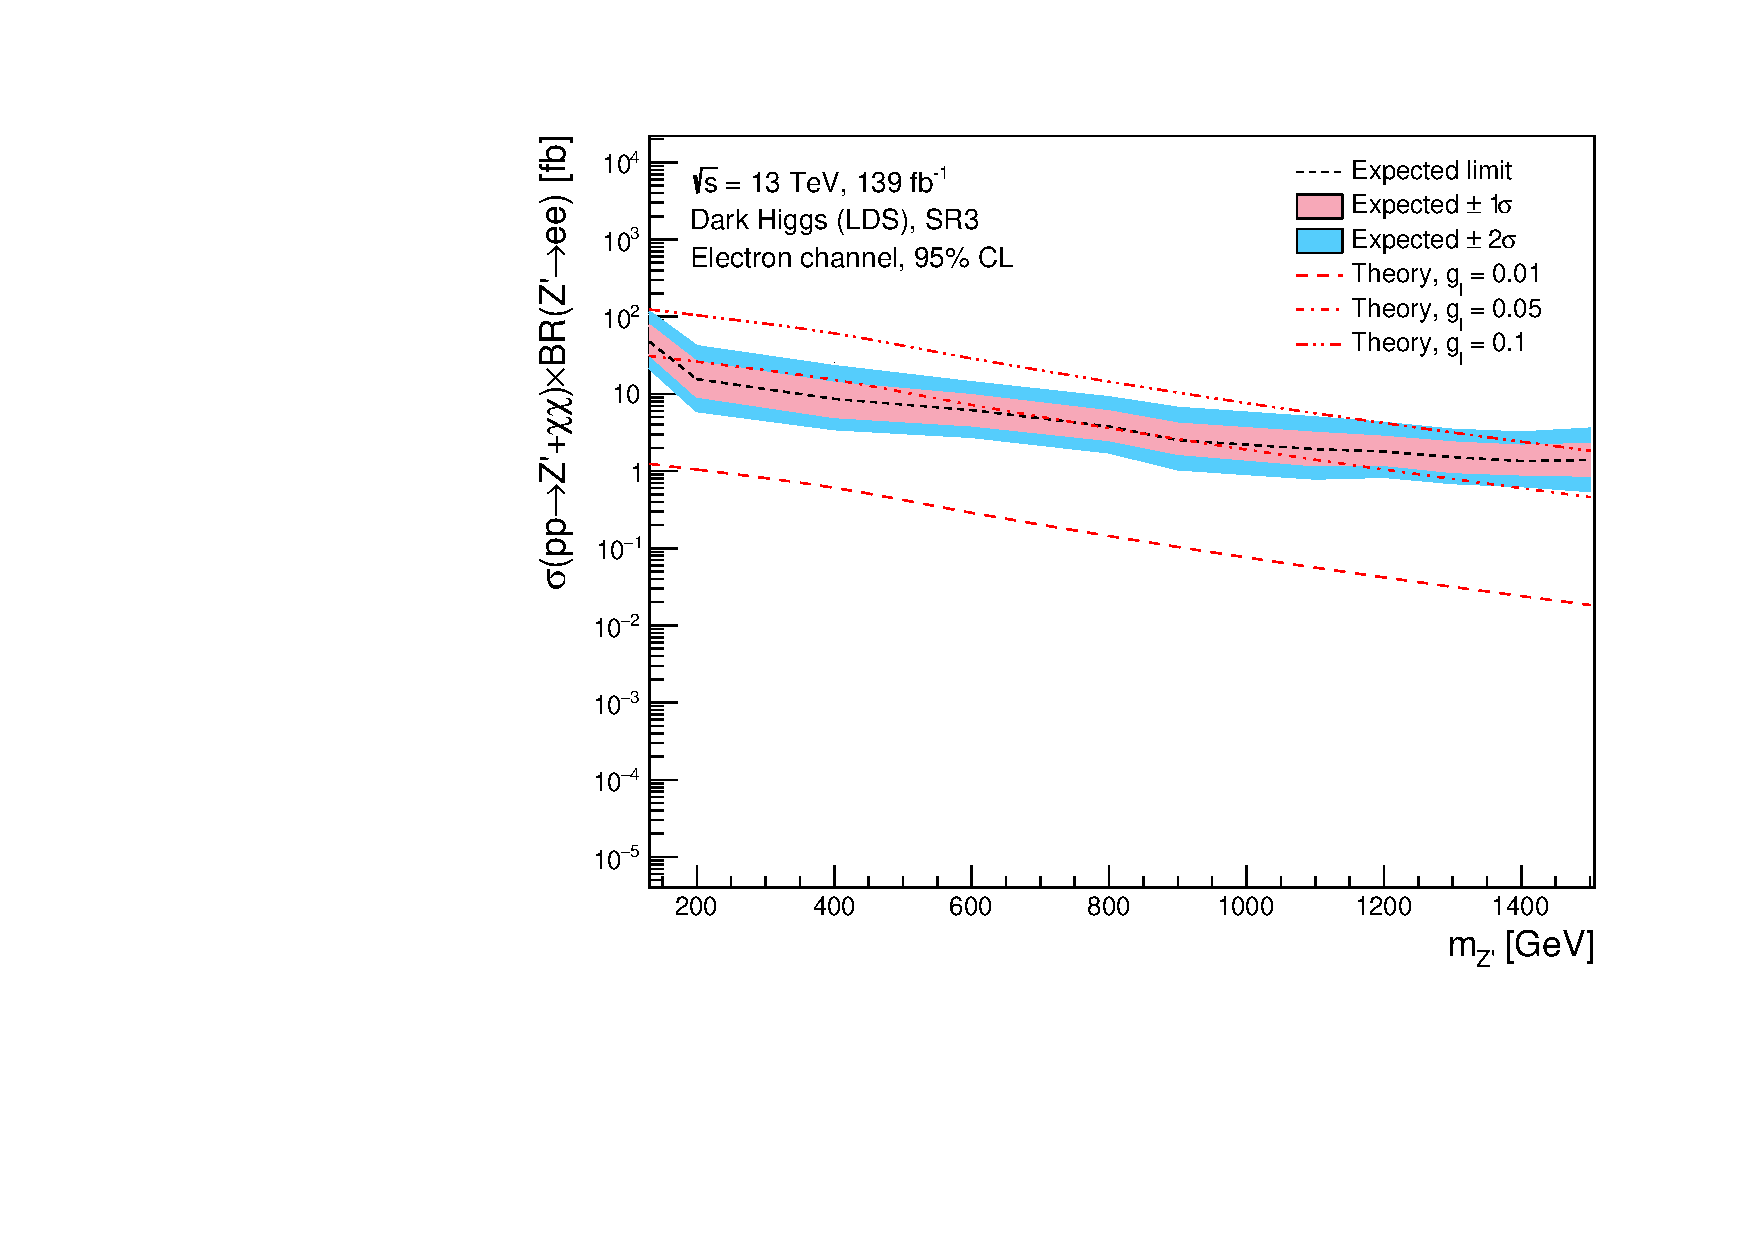
\includegraphics[width=1\textwidth]{Limits/Model_independent/150/DH_LDS/mass_exclusion_ee.pdf}
   \end{subfigure}
   \hfill
   \begin{subfigure}[b]{0.49\textwidth}
      \centering
      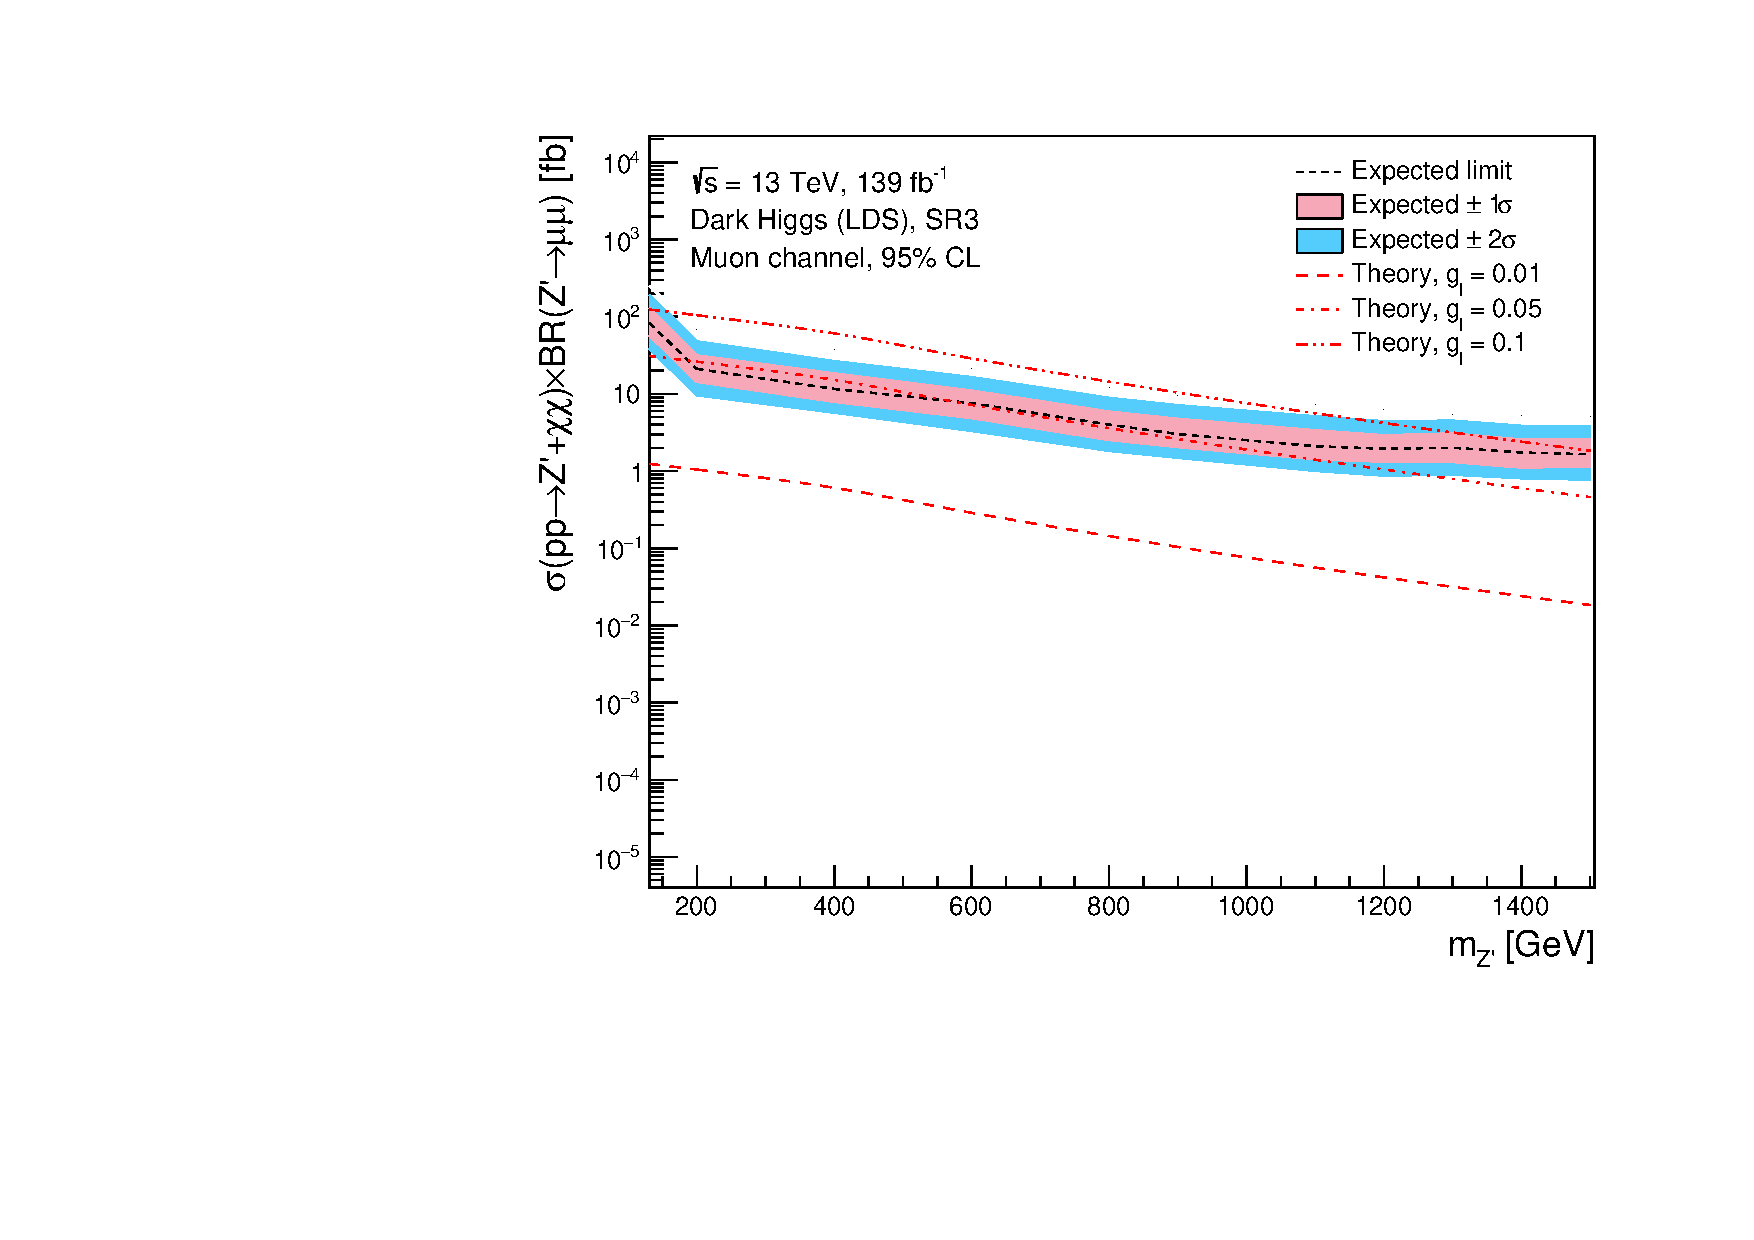
\includegraphics[width=1\textwidth]{Limits/Model_independent/150/DH_LDS/mass_exclusion_uu.pdf}
   \end{subfigure}
   \caption{Mass exclusiion limits results for DH LDS model on $ee$ and $\mu\mu$ channel in all SRs}\label{fig:DH_LDS_me_SRS}
\end{figure}

\begin{figure}[!ht]
	\centering
	\begin{subfigure}[b]{0.49\textwidth}
      \centering
      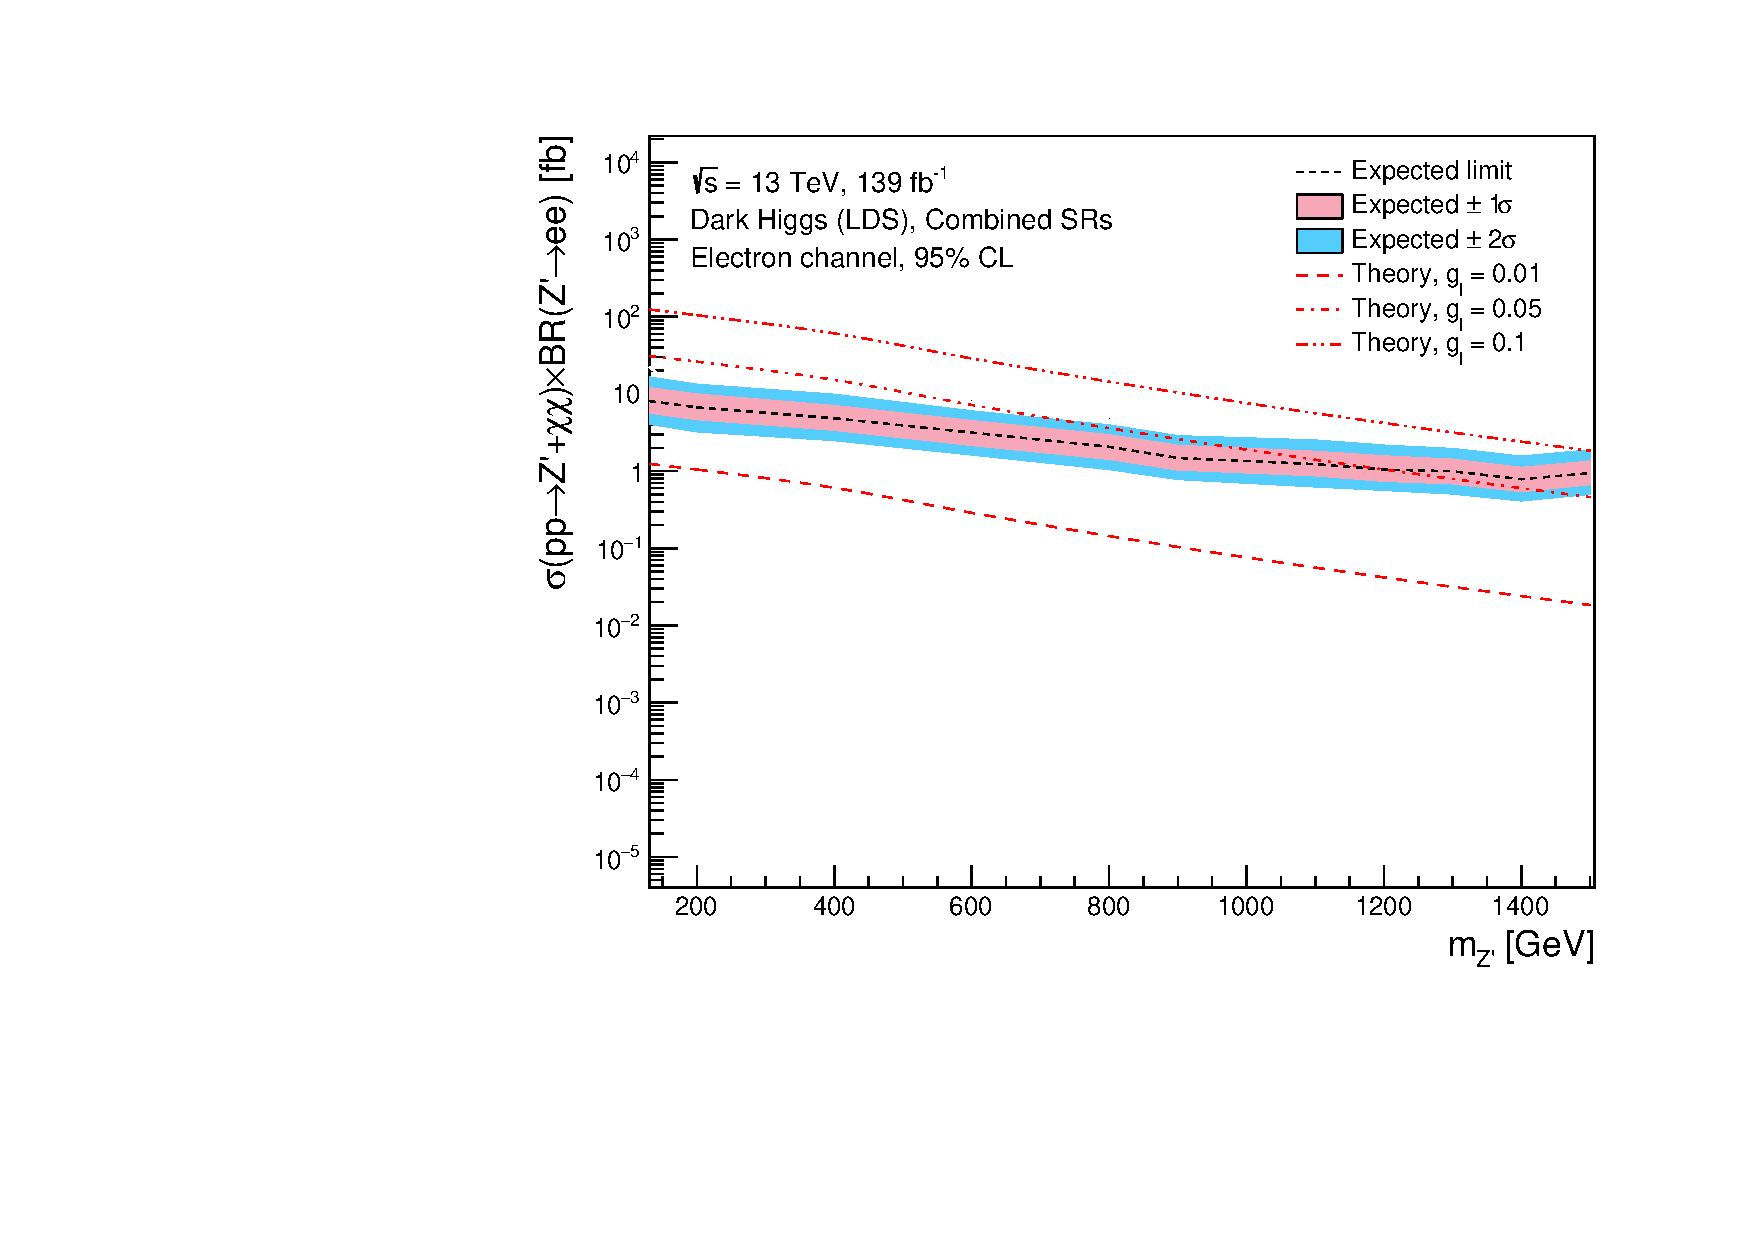
\includegraphics[width=1\textwidth]{Limits/Model_independent/DH_LDS/mass_exclusion_ee.pdf}
   \end{subfigure}
   \hfill
   \begin{subfigure}[b]{0.49\textwidth}
      \centering
      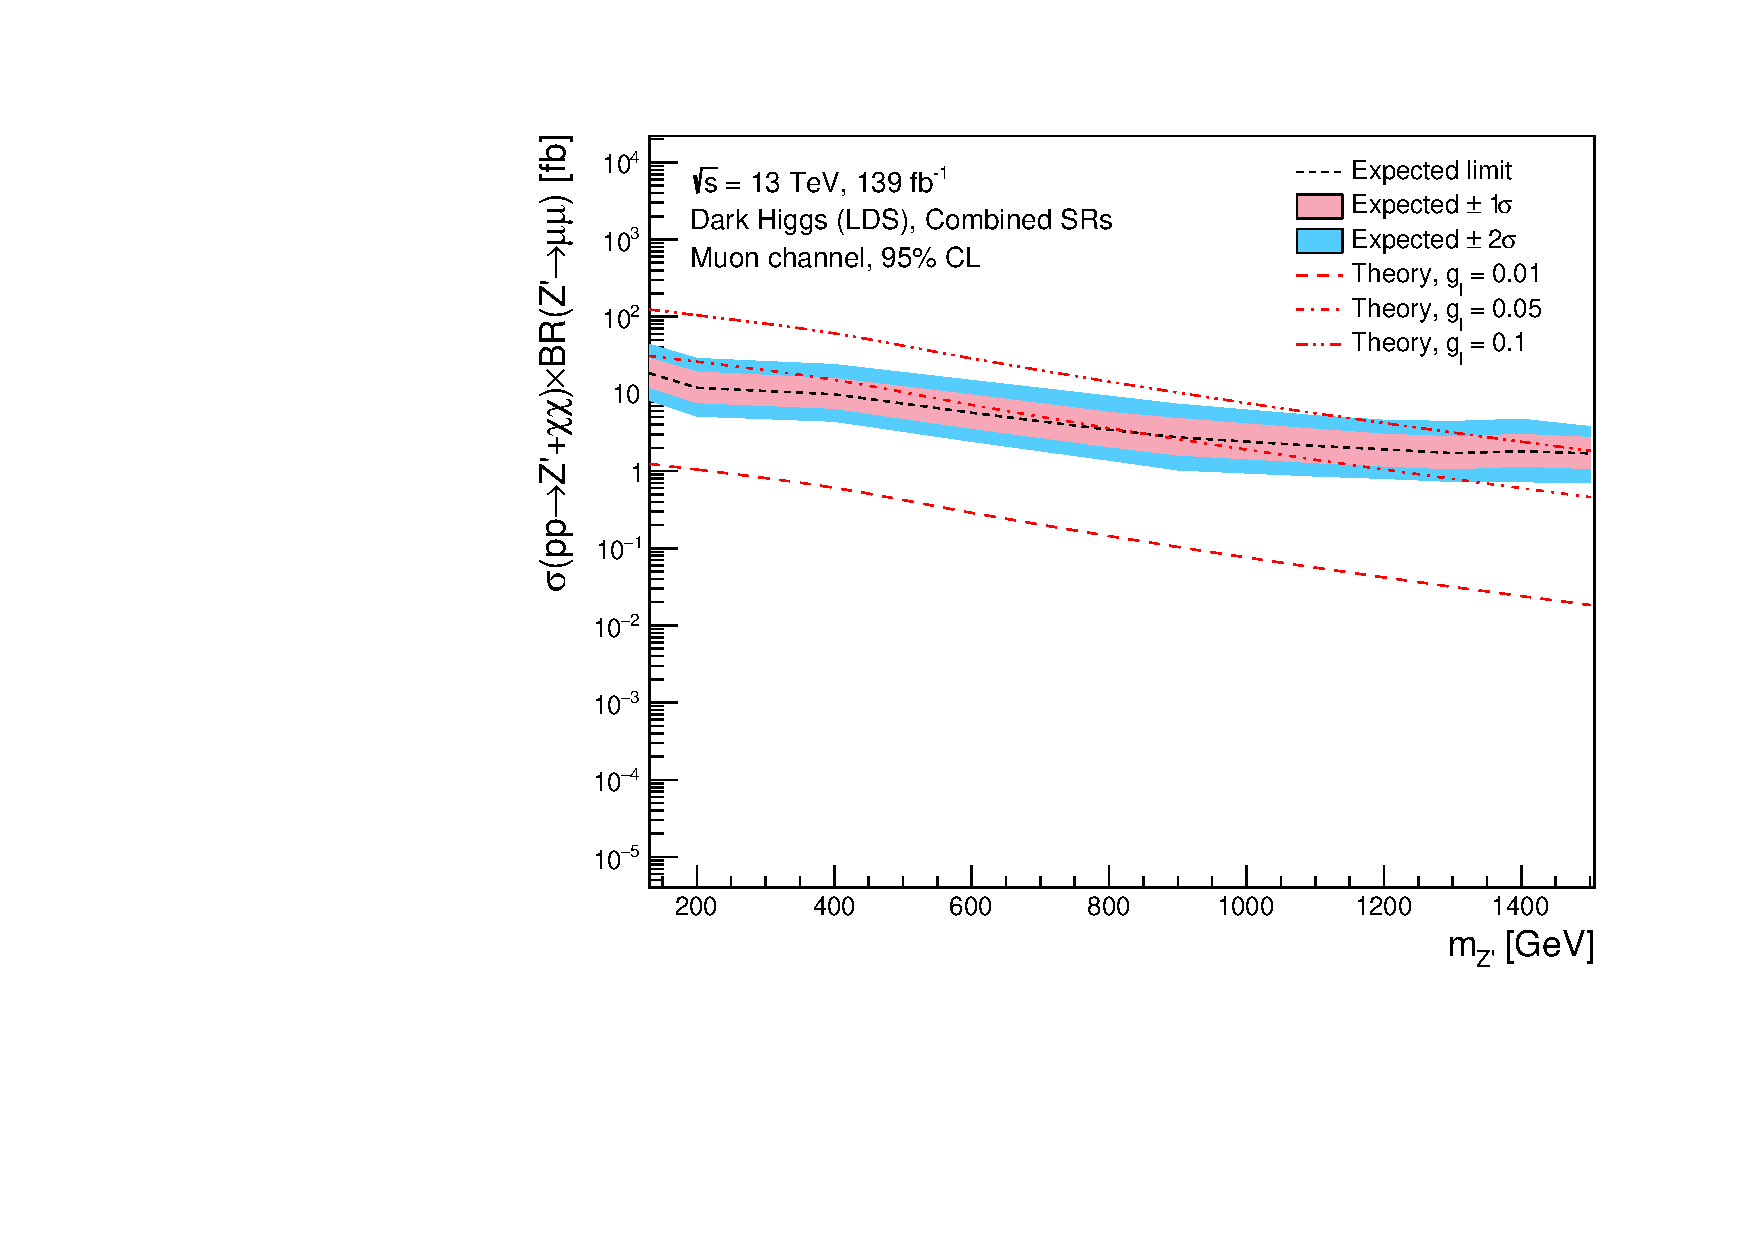
\includegraphics[width=1\textwidth]{Limits/Model_independent/DH_LDS/mass_exclusion_uu.pdf}
   \end{subfigure}
   \caption{Mass exclusiion limits results for DH LDS model on $ee$ and $\mu\mu$ channel in combined SRs}\label{fig:DH_LDS_me_comb}
\end{figure}

\clearpage

\section{Light Vector Heavy Dark Sector}
\begin{figure}[!ht]
	\centering
	\begin{subfigure}[b]{0.49\textwidth}
      \centering
      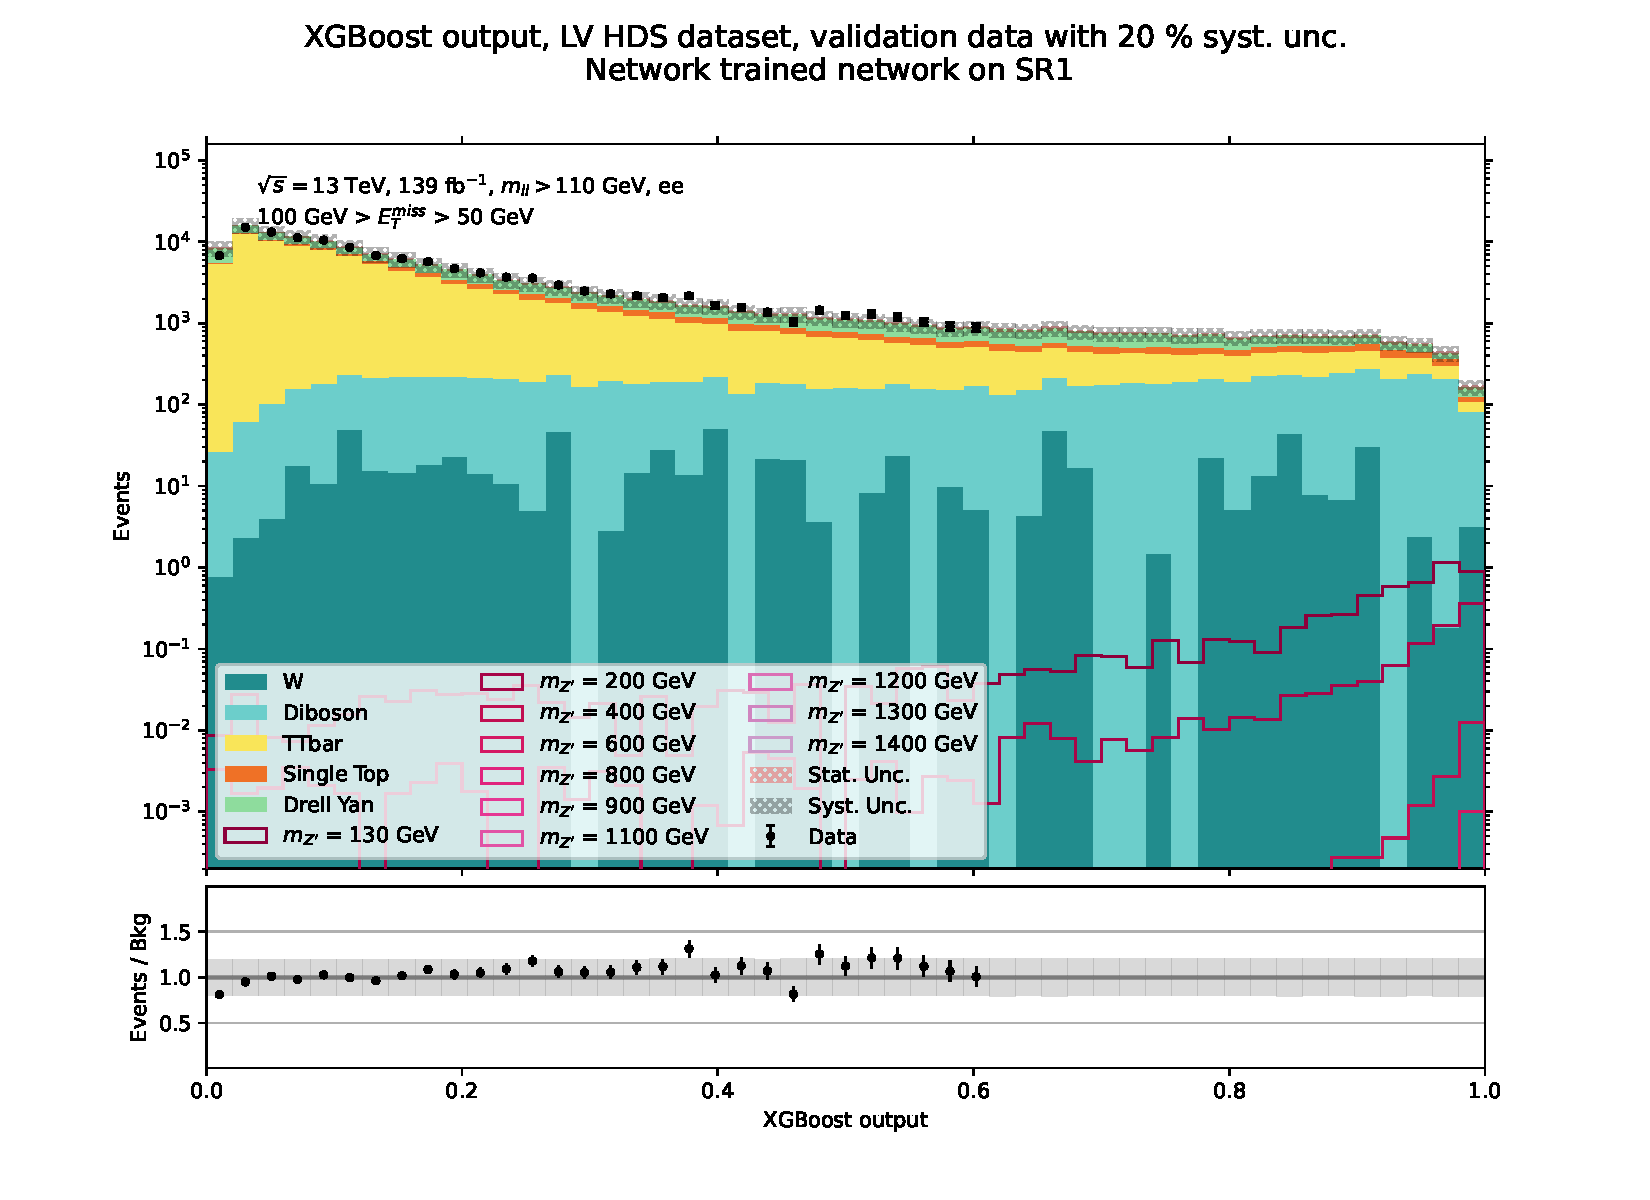
\includegraphics[width=1\textwidth]{XGBoost/Model_independent/50-100/LV_HDS/VAL_ee.pdf}
   \end{subfigure}
   \hfill
   \begin{subfigure}[b]{0.49\textwidth}
      \centering
      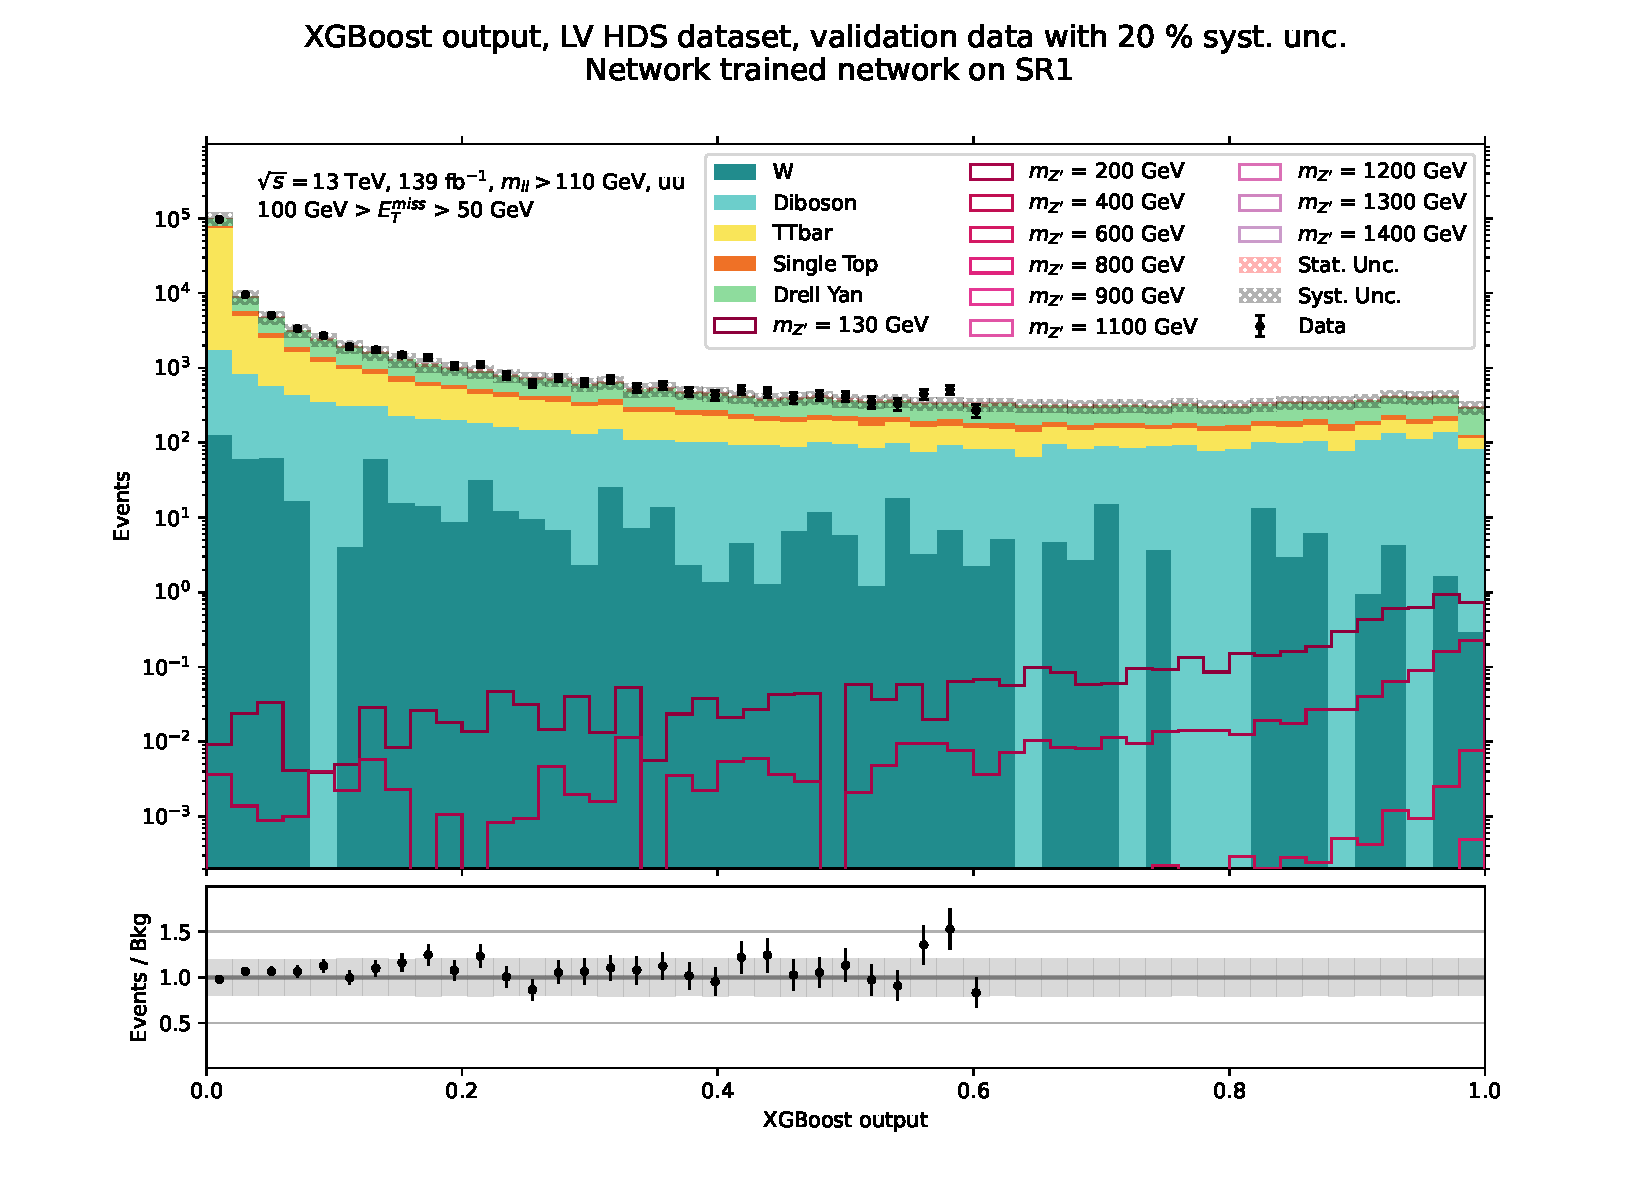
\includegraphics[width=1\textwidth]{XGBoost/Model_independent/50-100/LV_HDS/VAL_uu.pdf}
   \end{subfigure}
   \hfill
   \begin{subfigure}[b]{0.49\textwidth}
      \centering
      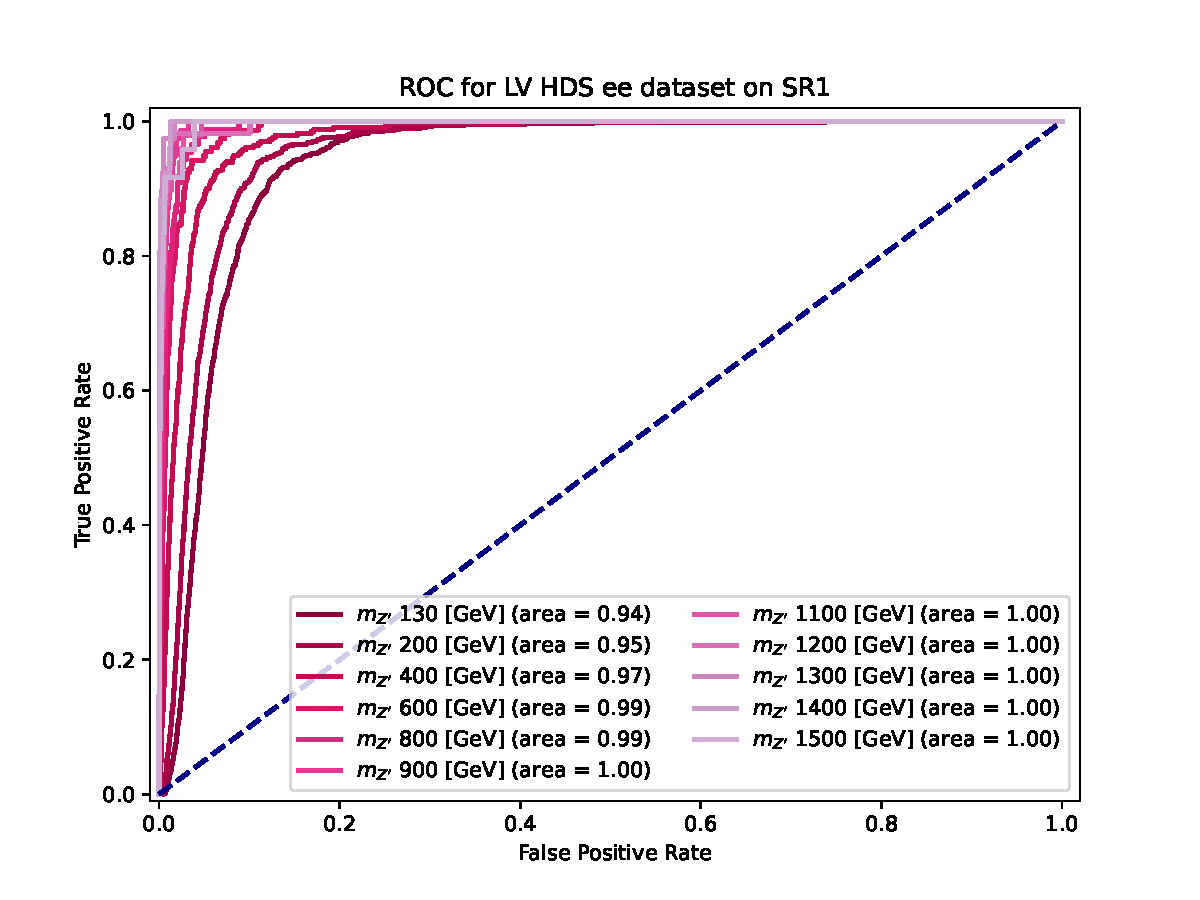
\includegraphics[width=1\textwidth]{XGBoost/Model_independent/50-100/LV_HDS/ROC_ee.pdf}
   \end{subfigure}
   \hfill
   \begin{subfigure}[b]{0.49\textwidth}
      \centering
      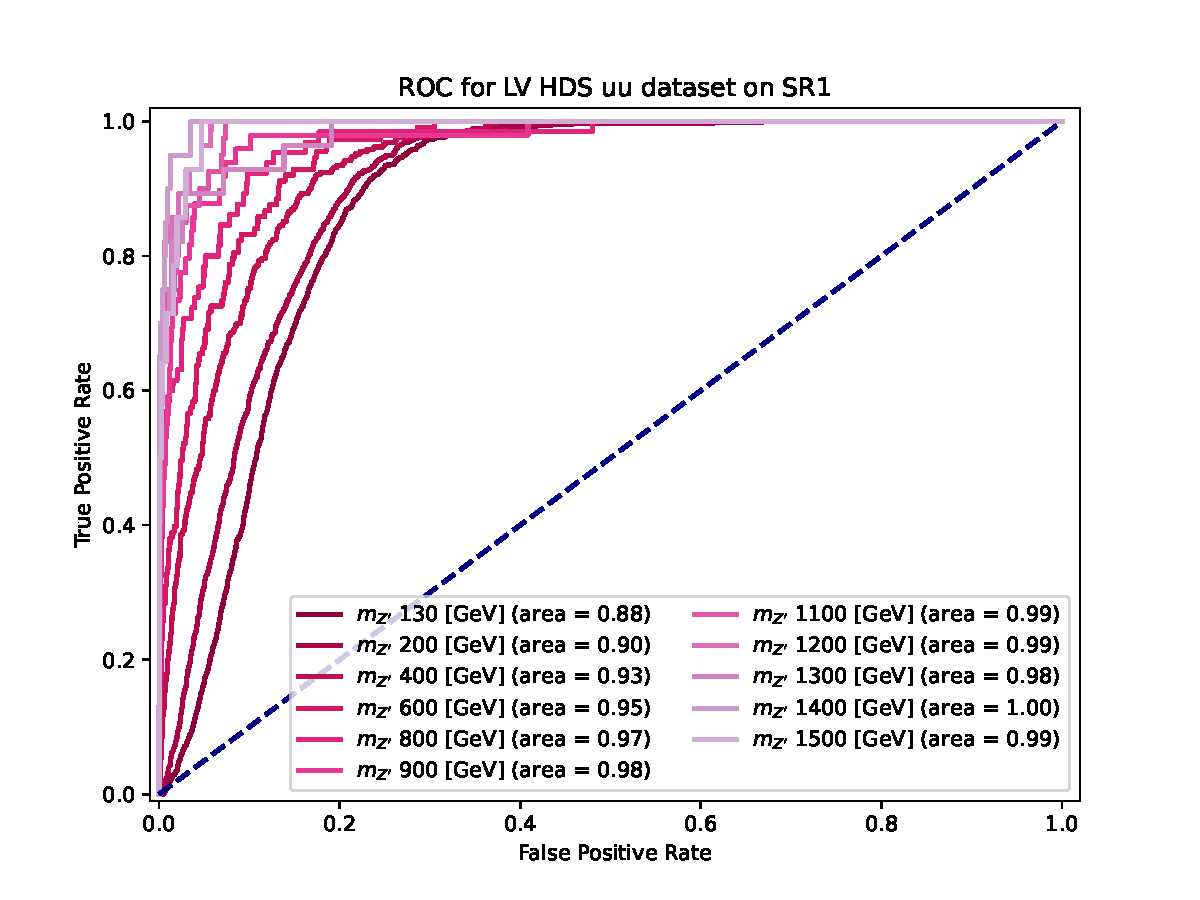
\includegraphics[width=1\textwidth]{XGBoost/Model_independent/50-100/LV_HDS/ROC_uu.pdf}
   \end{subfigure}
   \hfill
	\begin{subfigure}[b]{0.49\textwidth}
      \centering
      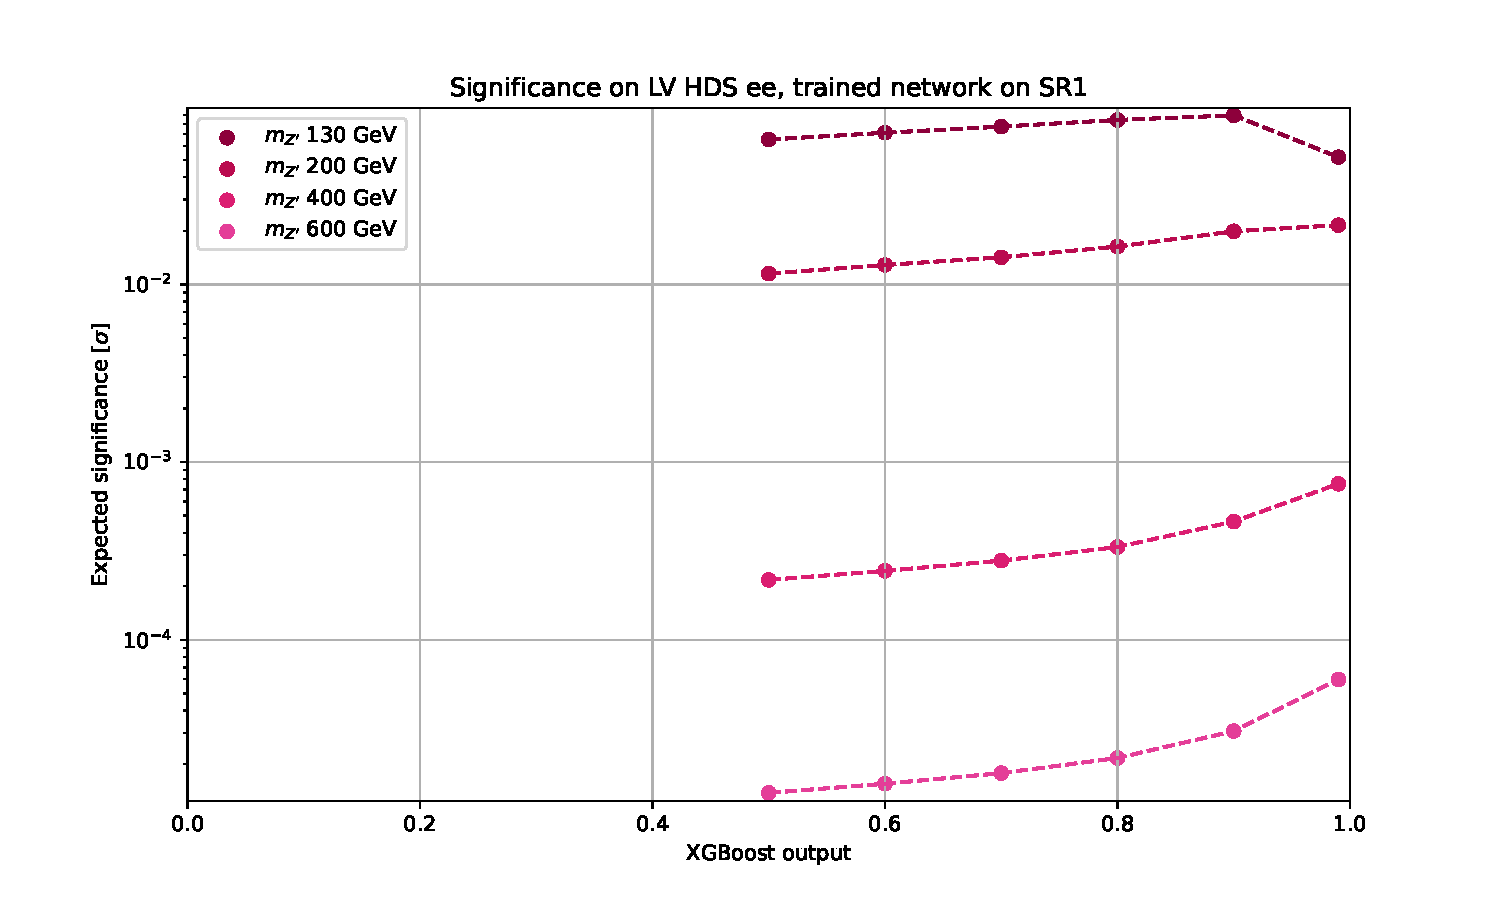
\includegraphics[width=1\textwidth]{XGBoost/Model_independent/50-100/LV_HDS/EXP_SIG_ee.pdf}
   \end{subfigure}
   \hfill
   \begin{subfigure}[b]{0.49\textwidth}
      \centering
      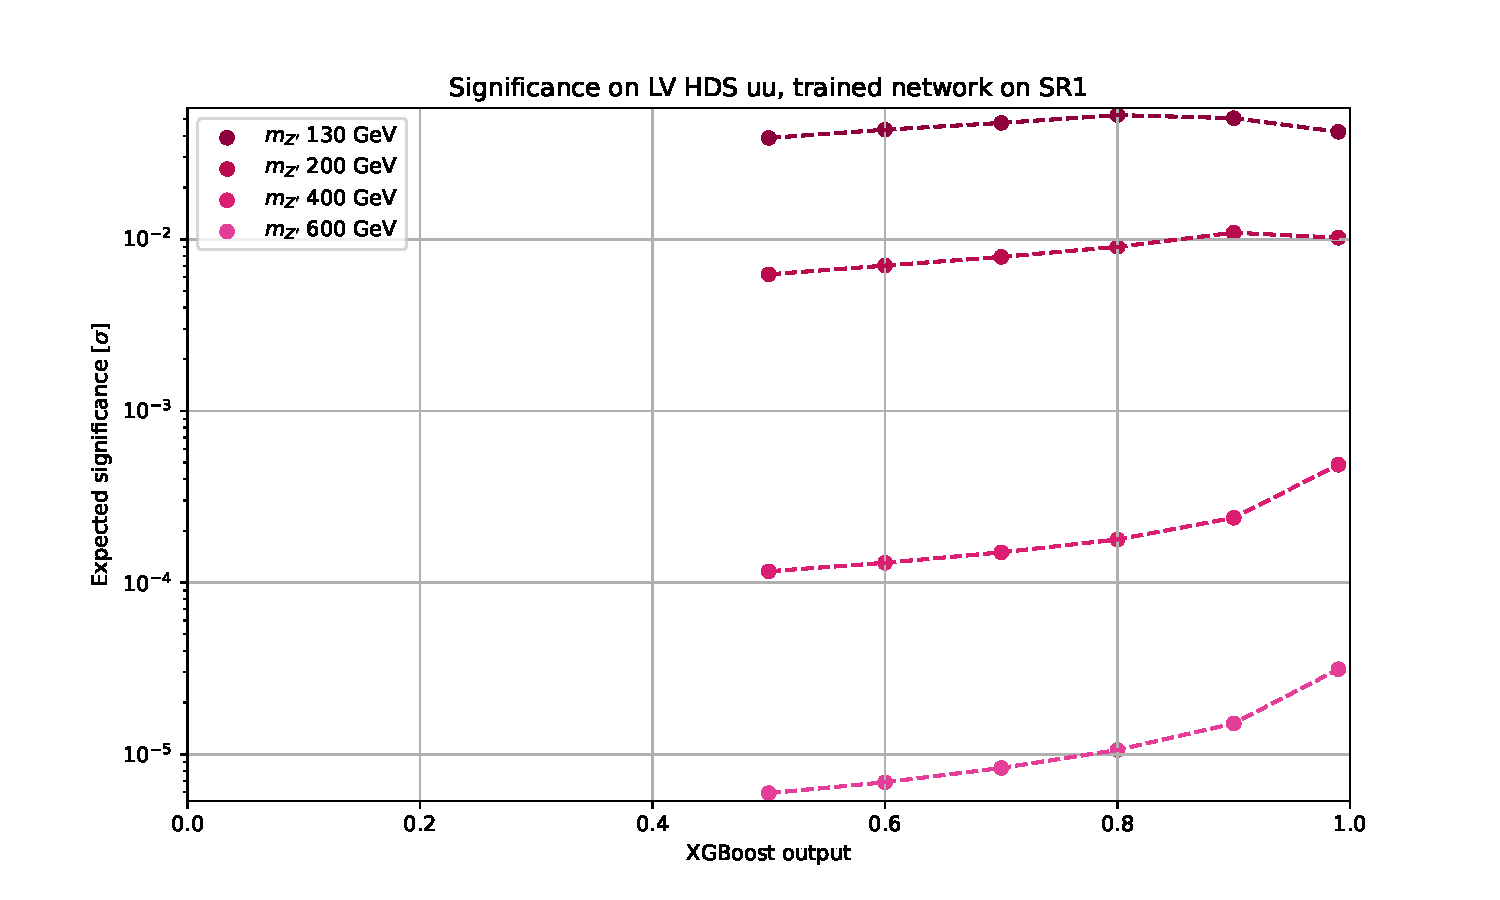
\includegraphics[width=1\textwidth]{XGBoost/Model_independent/50-100/LV_HDS/EXP_SIG_uu.pdf}
   \end{subfigure}
   \caption{XGBoost results for LV HDS model on $ee$ and $\mu\mu$ channel in SR1}\label{fig:LV_HDS_SR1}
\end{figure}

\begin{figure}[!ht]
	\centering
	\begin{subfigure}[b]{0.49\textwidth}
      \centering
      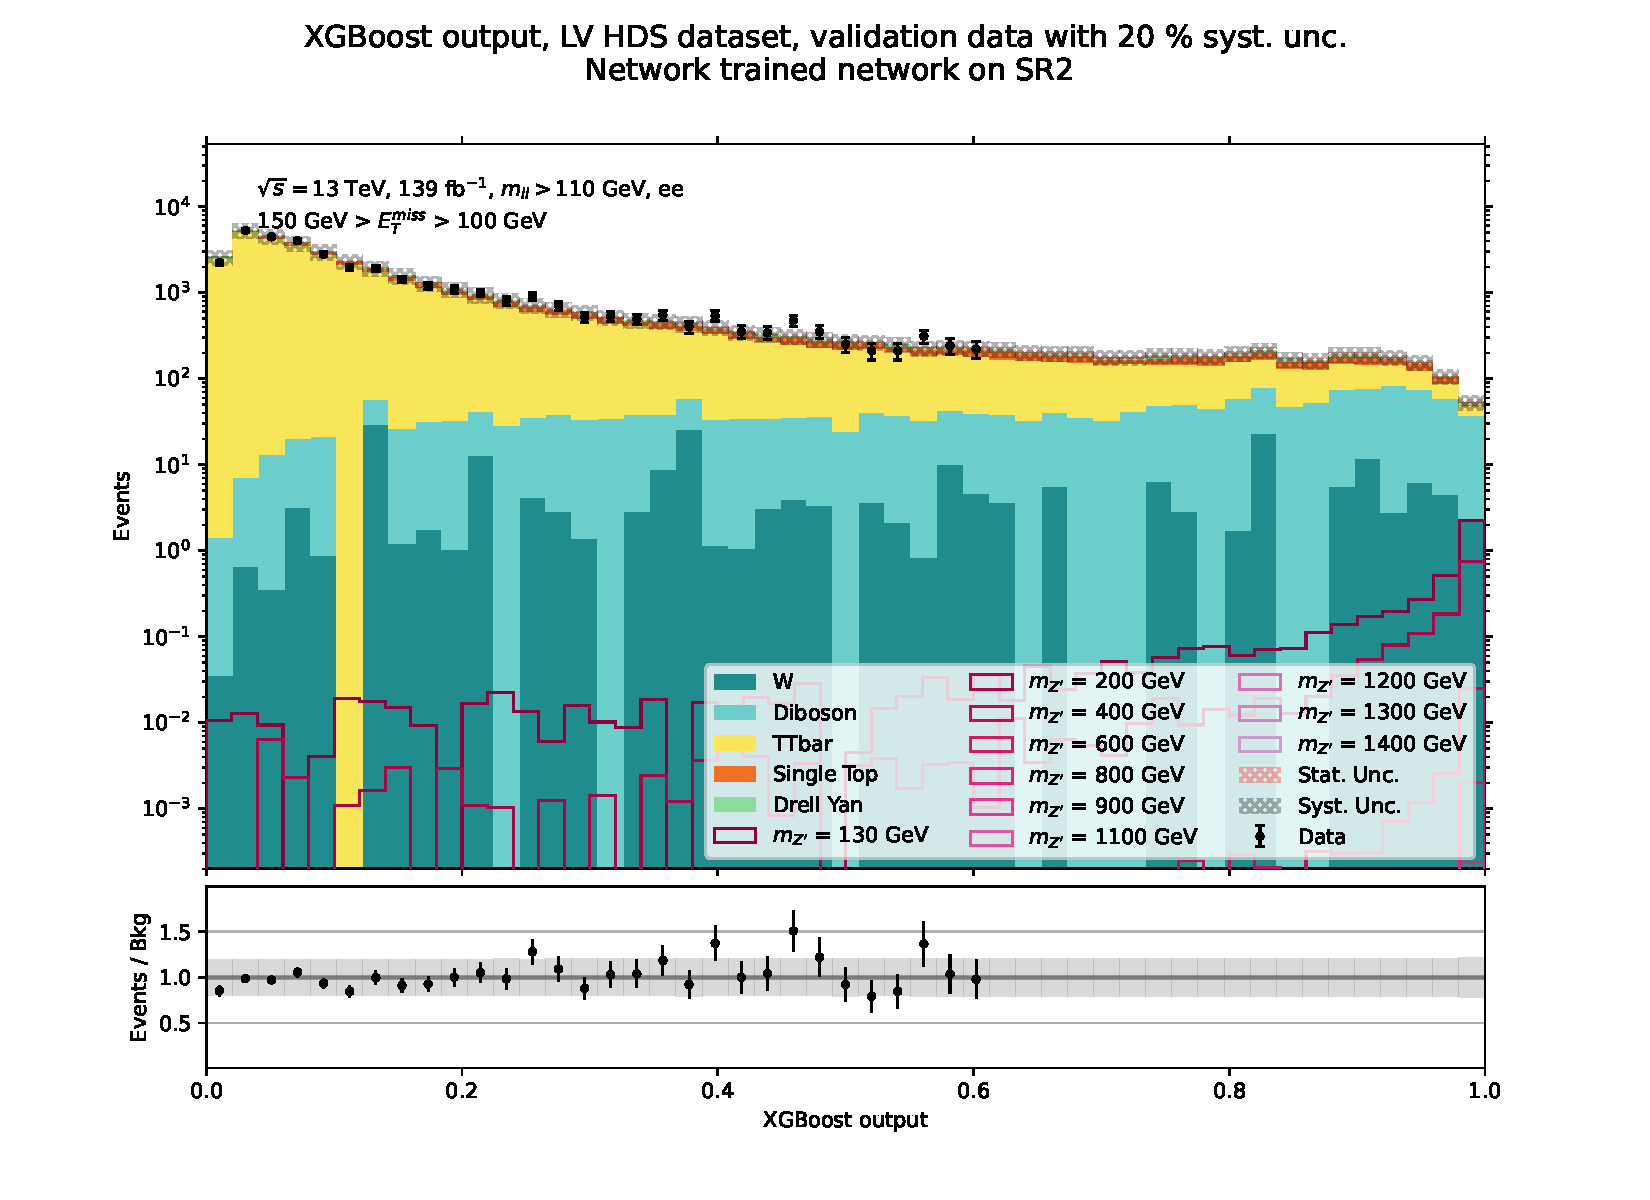
\includegraphics[width=1\textwidth]{XGBoost/Model_independent/100-150/LV_HDS/VAL_ee.pdf}
   \end{subfigure}
   \hfill
   \begin{subfigure}[b]{0.49\textwidth}
      \centering
      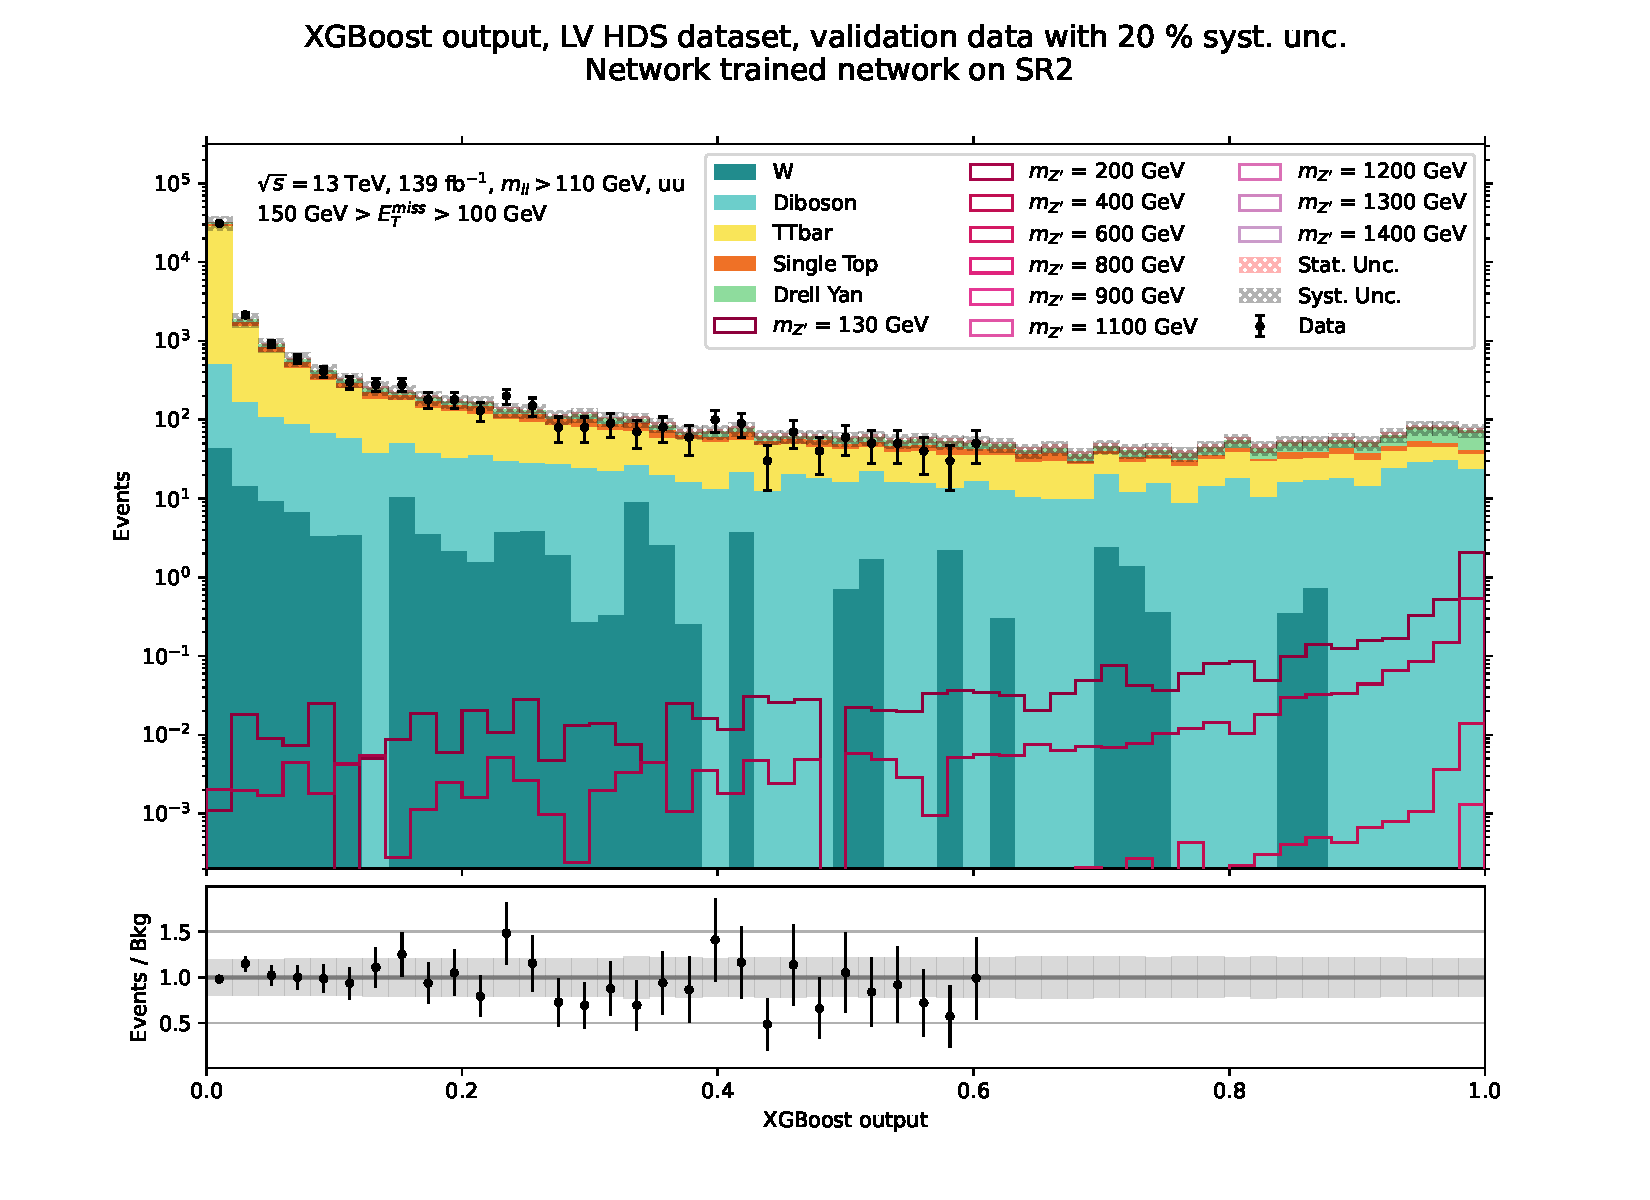
\includegraphics[width=1\textwidth]{XGBoost/Model_independent/100-150/LV_HDS/VAL_uu.pdf}
   \end{subfigure}
   \hfill
   \begin{subfigure}[b]{0.49\textwidth}
      \centering
      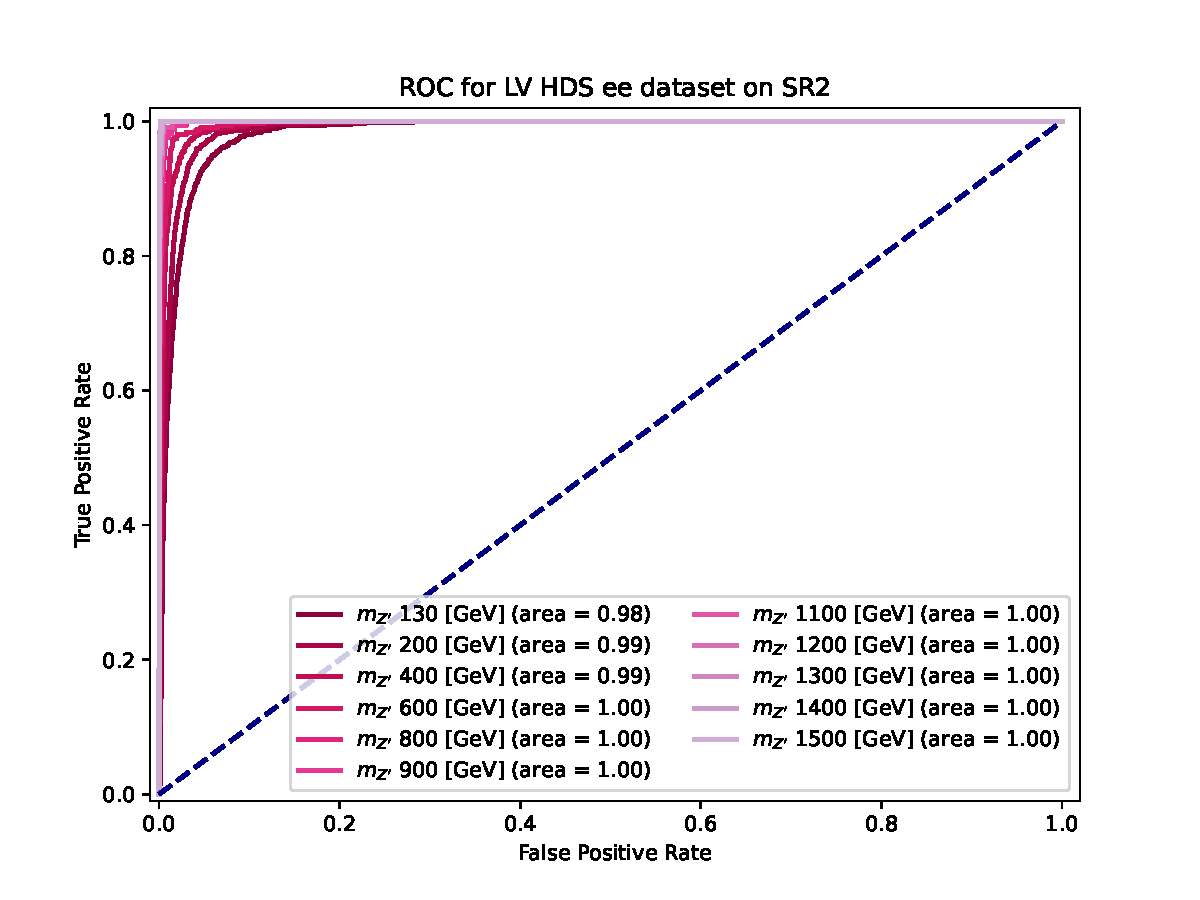
\includegraphics[width=1\textwidth]{XGBoost/Model_independent/100-150/LV_HDS/ROC_ee.pdf}
   \end{subfigure}
   \hfill
   \begin{subfigure}[b]{0.49\textwidth}
      \centering
      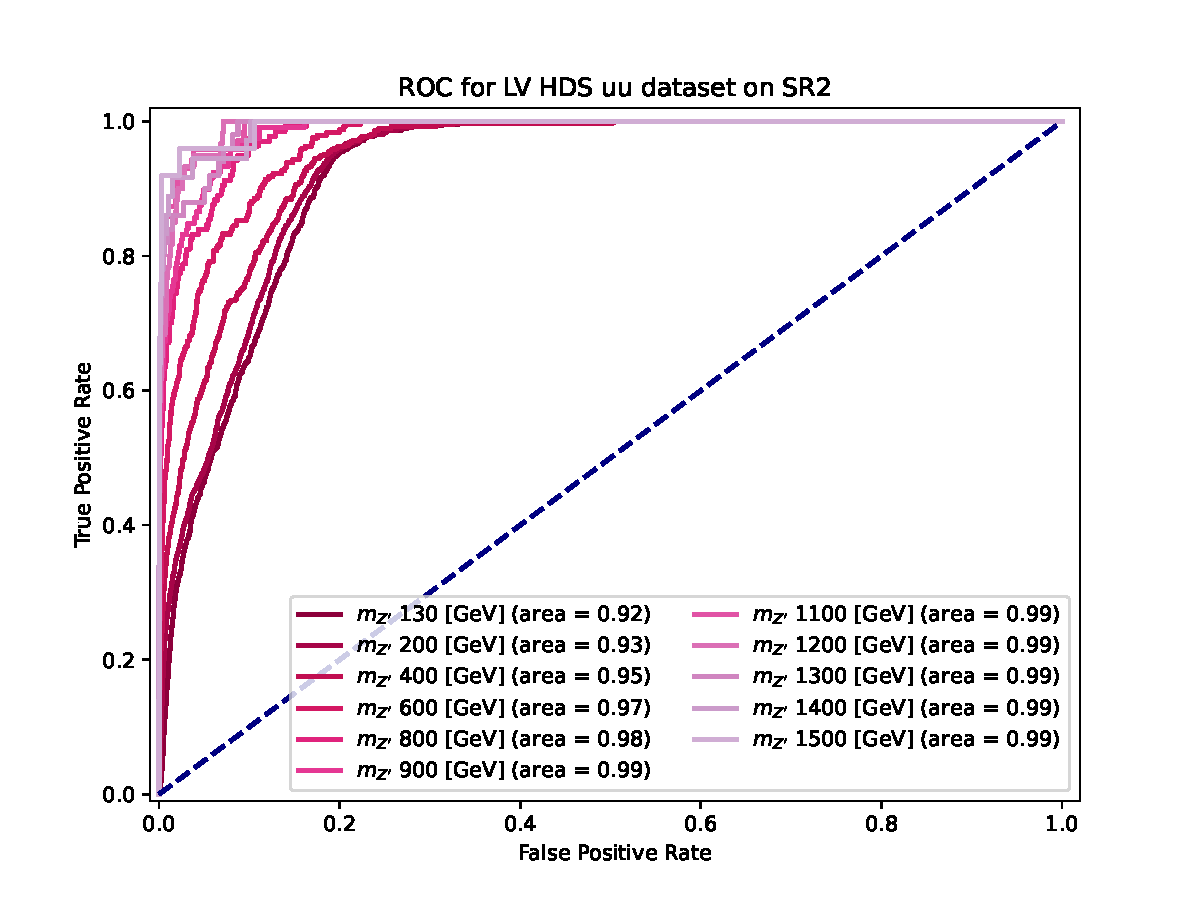
\includegraphics[width=1\textwidth]{XGBoost/Model_independent/100-150/LV_HDS/ROC_uu.pdf}
   \end{subfigure}
   \hfill
	\begin{subfigure}[b]{0.49\textwidth}
      \centering
      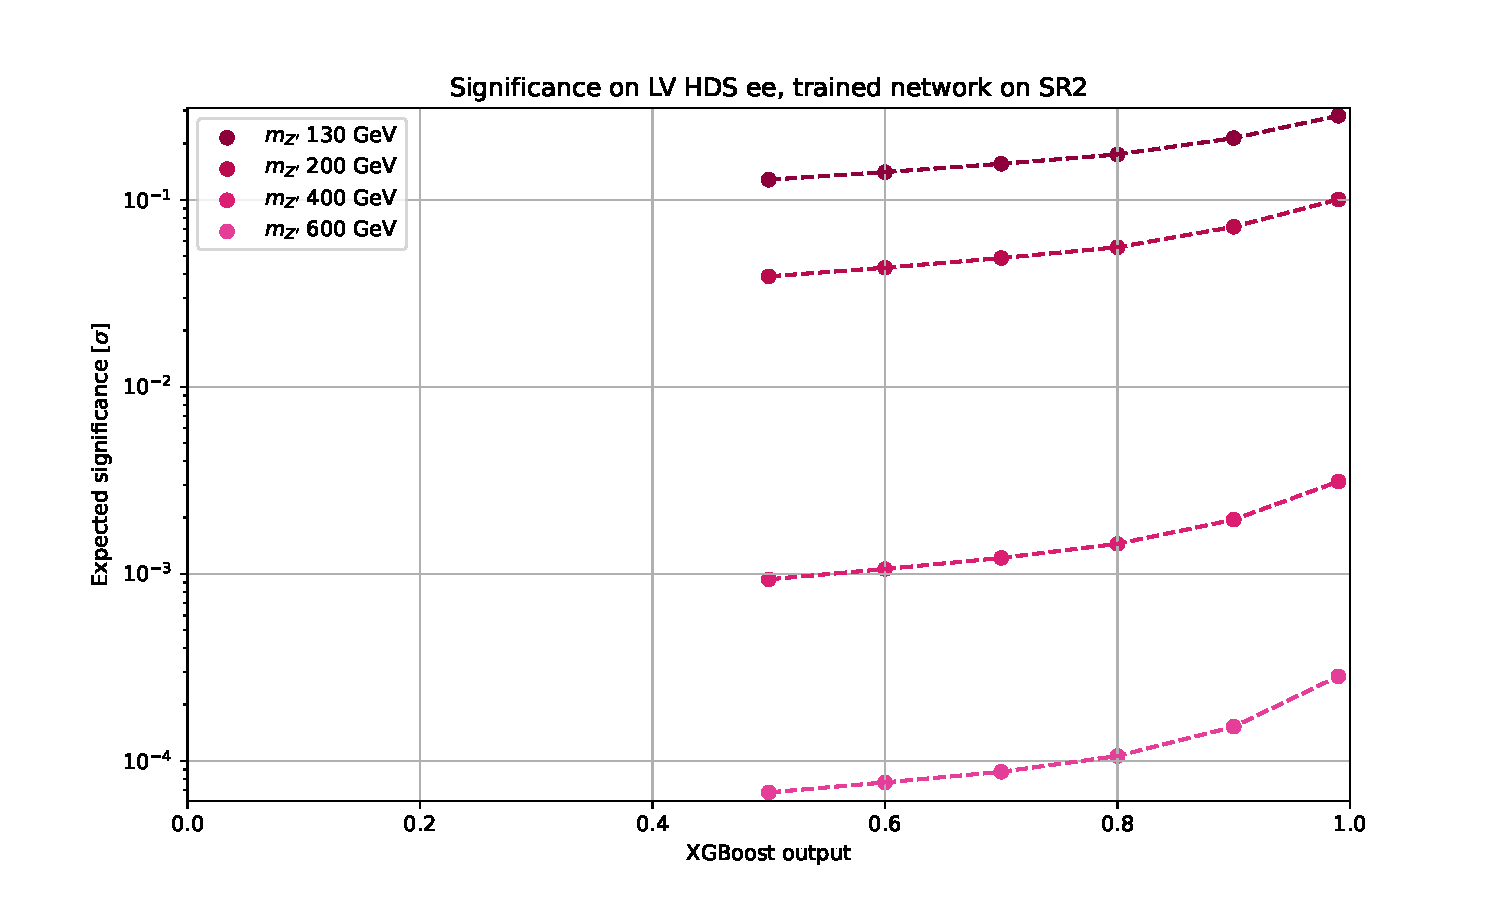
\includegraphics[width=1\textwidth]{XGBoost/Model_independent/100-150/LV_HDS/EXP_SIG_ee.pdf}
   \end{subfigure}
   \hfill
   \begin{subfigure}[b]{0.49\textwidth}
      \centering
      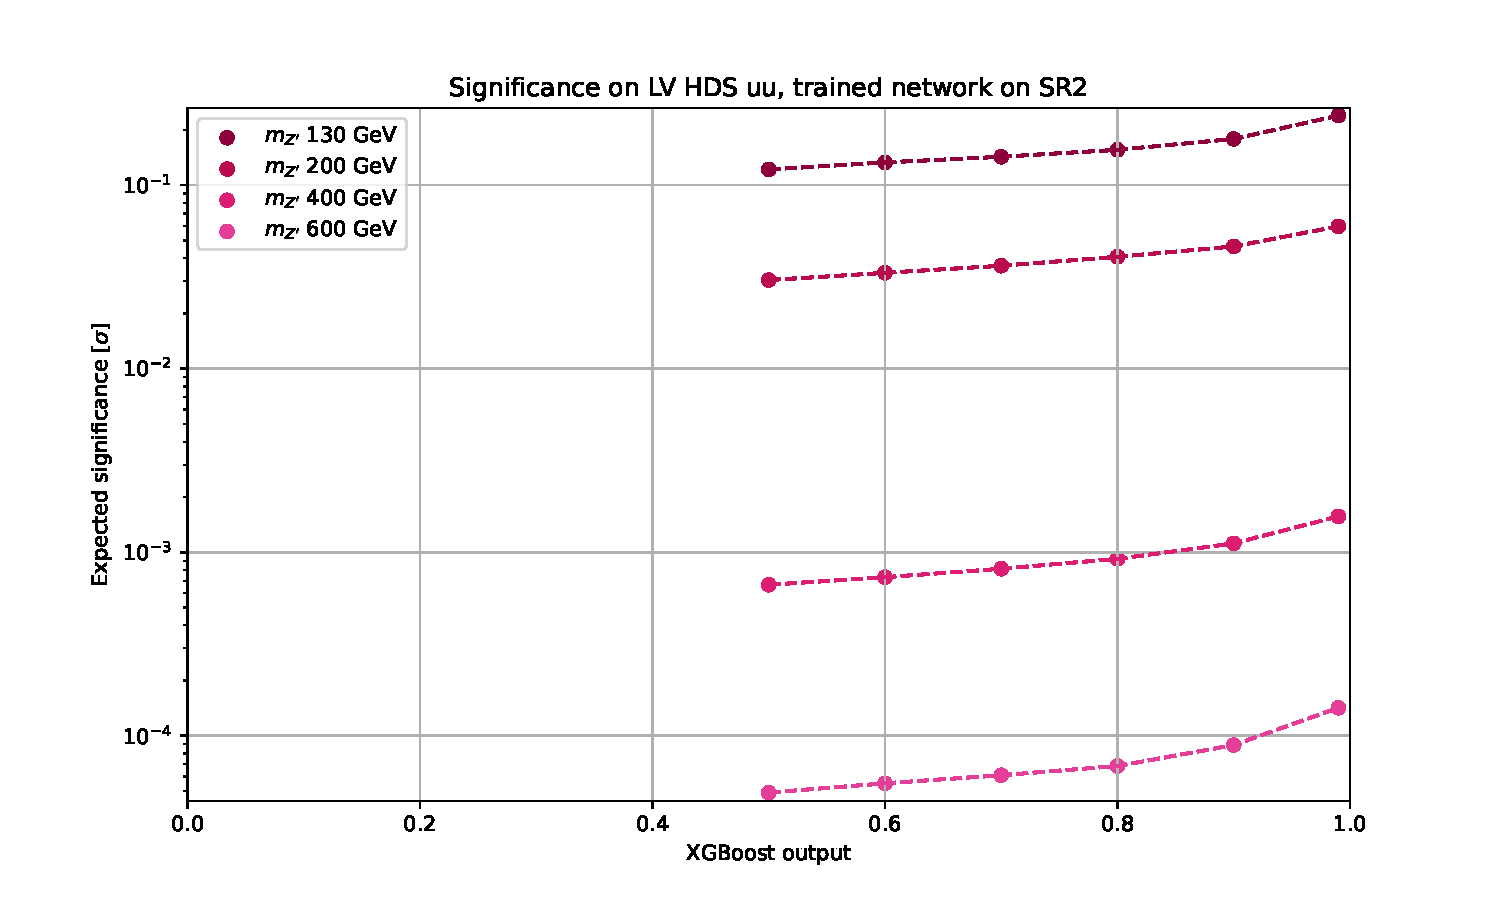
\includegraphics[width=1\textwidth]{XGBoost/Model_independent/100-150/LV_HDS/EXP_SIG_uu.pdf}
   \end{subfigure}
   \caption{XGBoost results for LV HDS model on $ee$ and $\mu\mu$ channel in SR2}\label{fig:LV_HDS_SR2}
\end{figure}

\begin{figure}[!ht]
	\centering
	\begin{subfigure}[b]{0.49\textwidth}
      \centering
      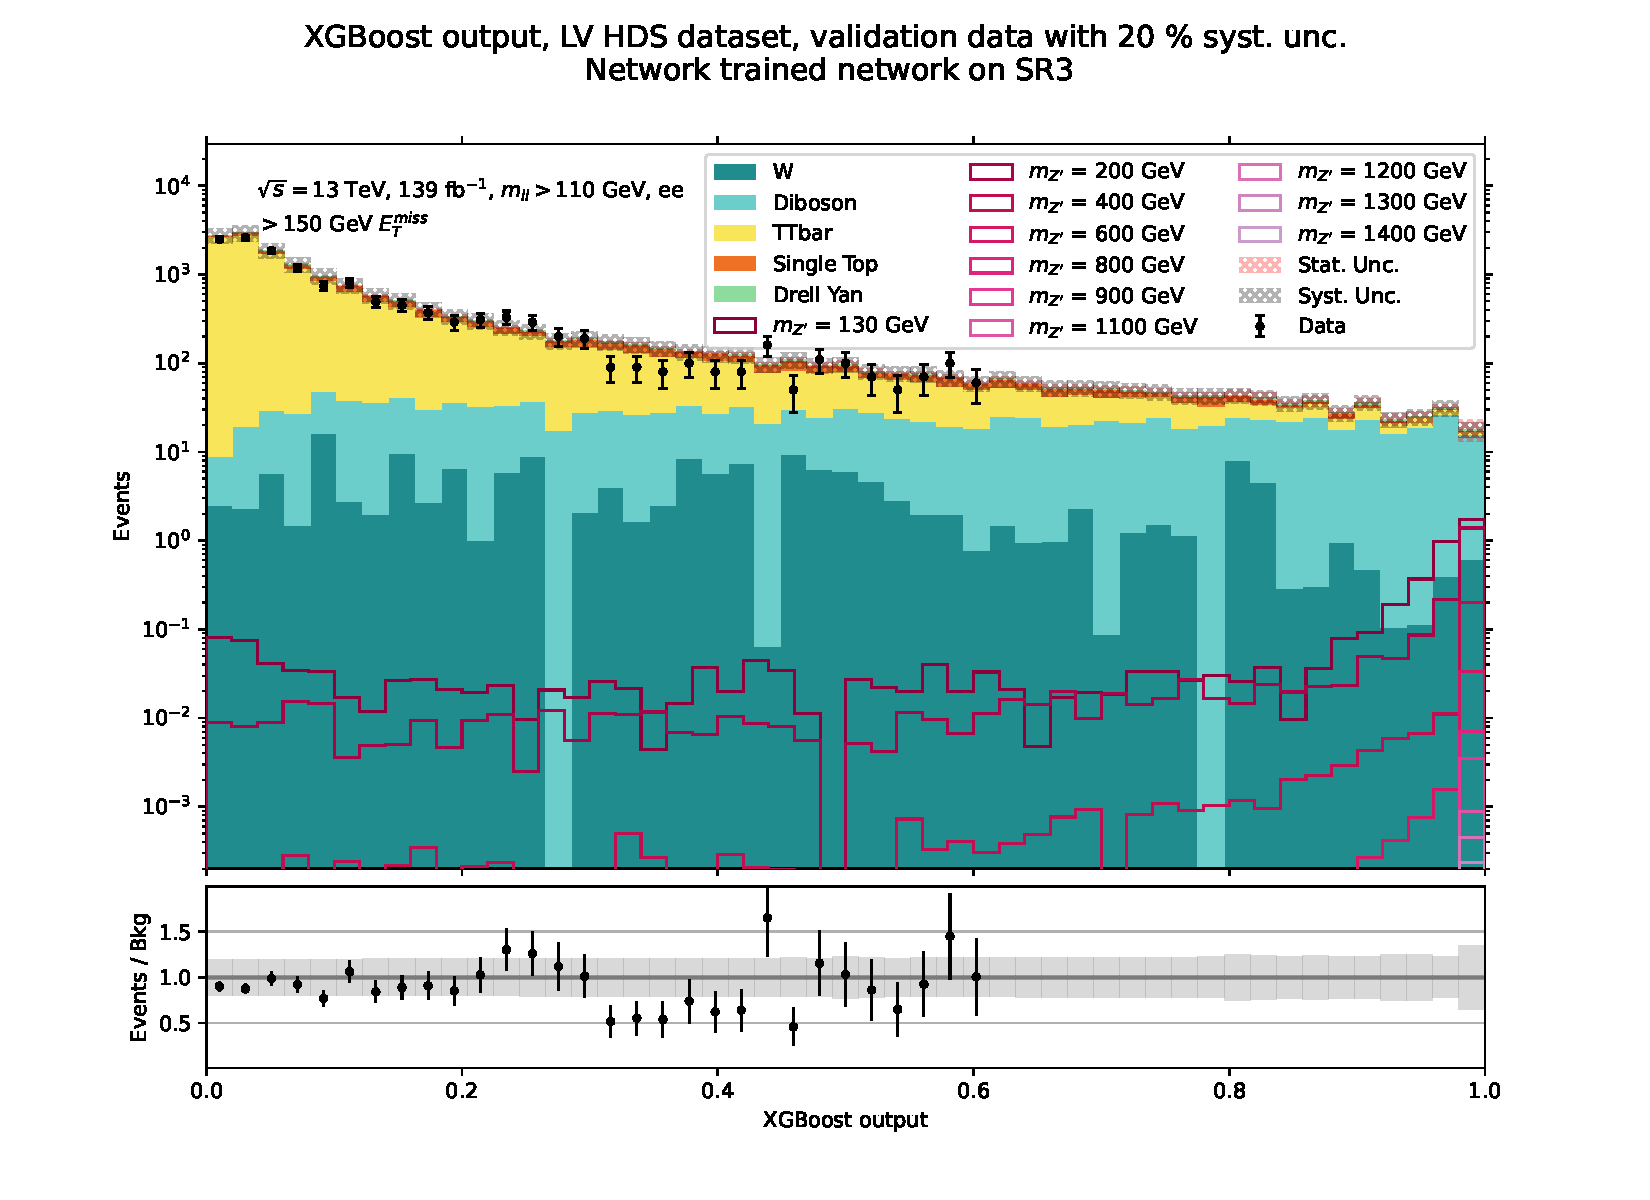
\includegraphics[width=1\textwidth]{XGBoost/Model_independent/150/LV_HDS/VAL_ee.pdf}
   \end{subfigure}
   \hfill
   \begin{subfigure}[b]{0.49\textwidth}
      \centering
      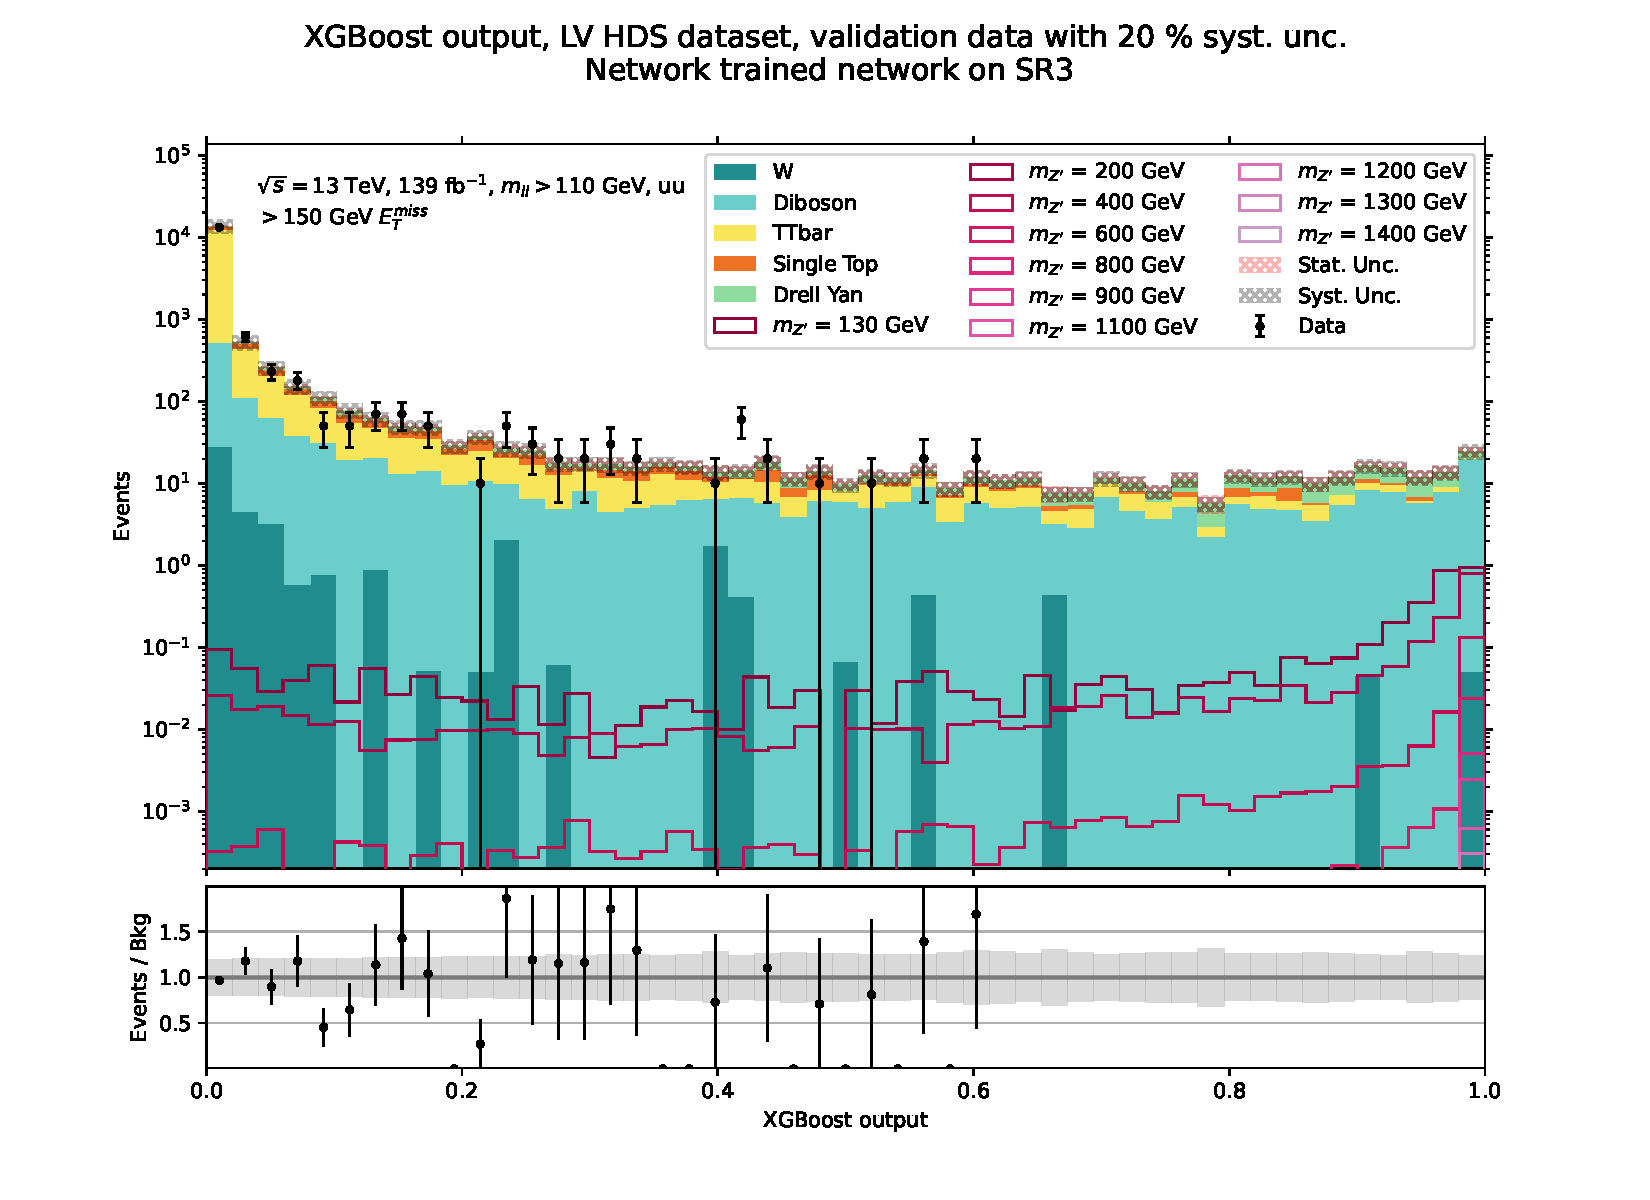
\includegraphics[width=1\textwidth]{XGBoost/Model_independent/150/LV_HDS/VAL_uu.pdf}
   \end{subfigure}
   \hfill
   \begin{subfigure}[b]{0.49\textwidth}
      \centering
      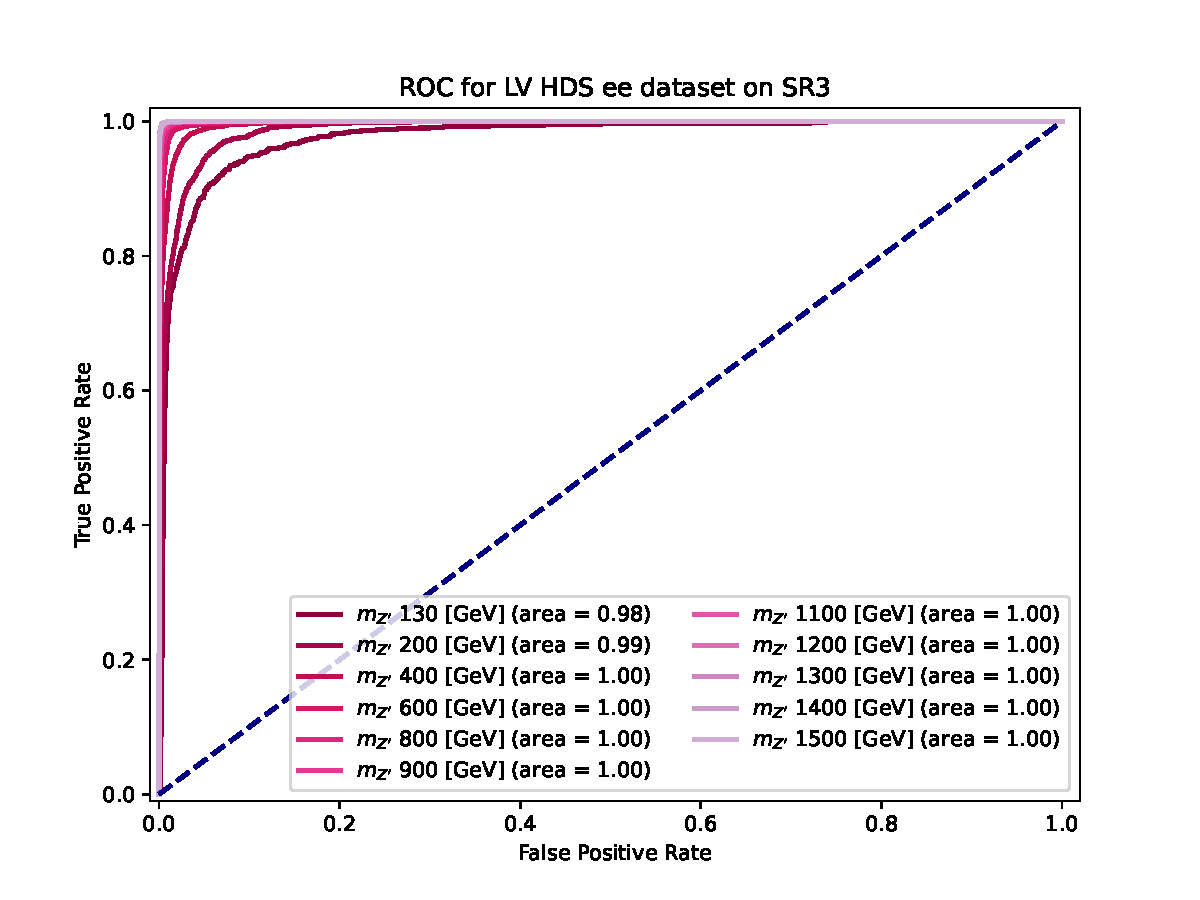
\includegraphics[width=1\textwidth]{XGBoost/Model_independent/150/LV_HDS/ROC_ee.pdf}
   \end{subfigure}
   \hfill
   \begin{subfigure}[b]{0.49\textwidth}
      \centering
      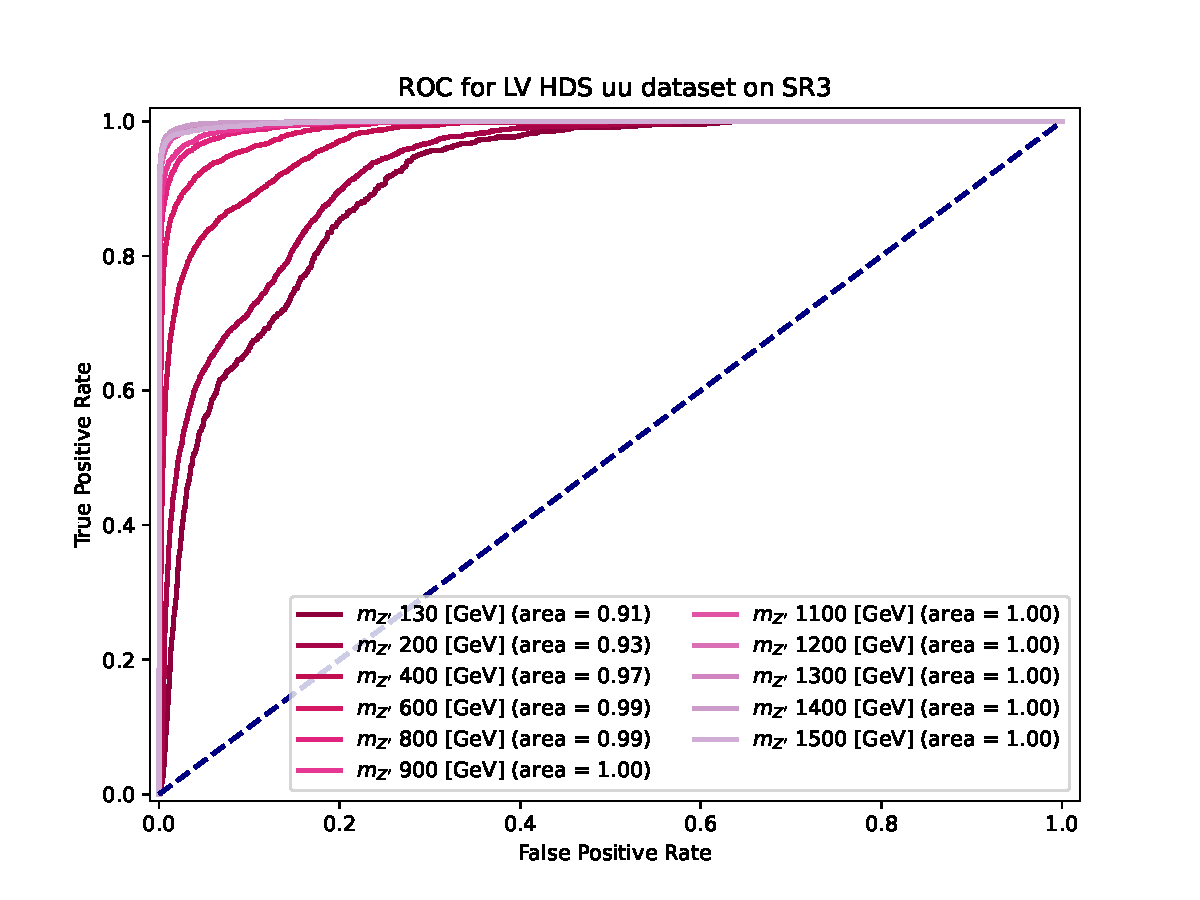
\includegraphics[width=1\textwidth]{XGBoost/Model_independent/150/LV_HDS/ROC_uu.pdf}
   \end{subfigure}
   \hfill
	\begin{subfigure}[b]{0.49\textwidth}
      \centering
      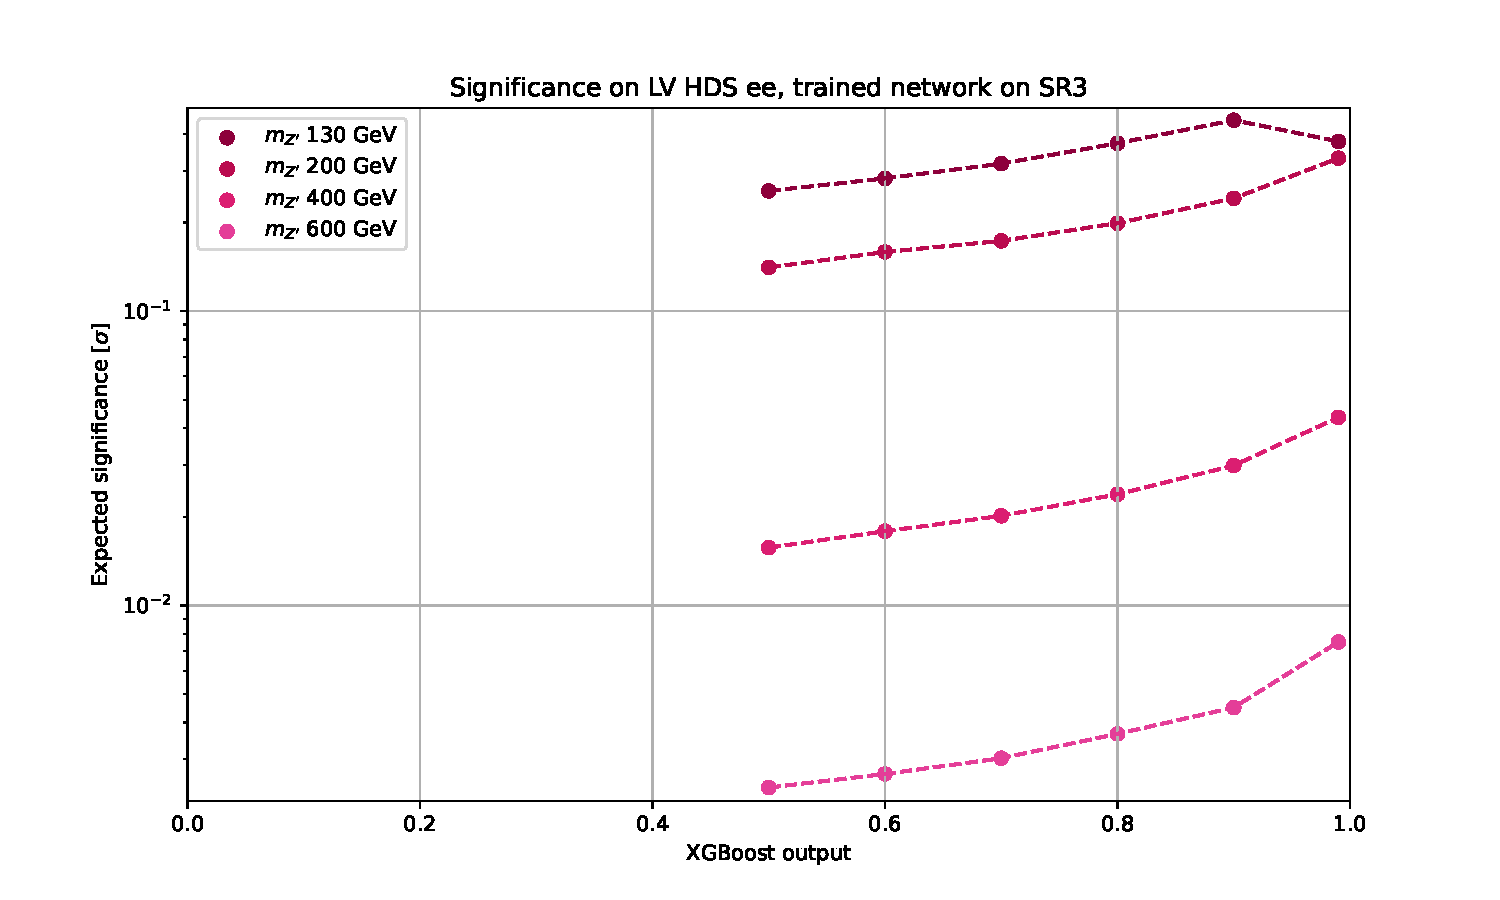
\includegraphics[width=1\textwidth]{XGBoost/Model_independent/150/LV_HDS/EXP_SIG_ee.pdf}
   \end{subfigure}
   \hfill
   \begin{subfigure}[b]{0.49\textwidth}
      \centering
      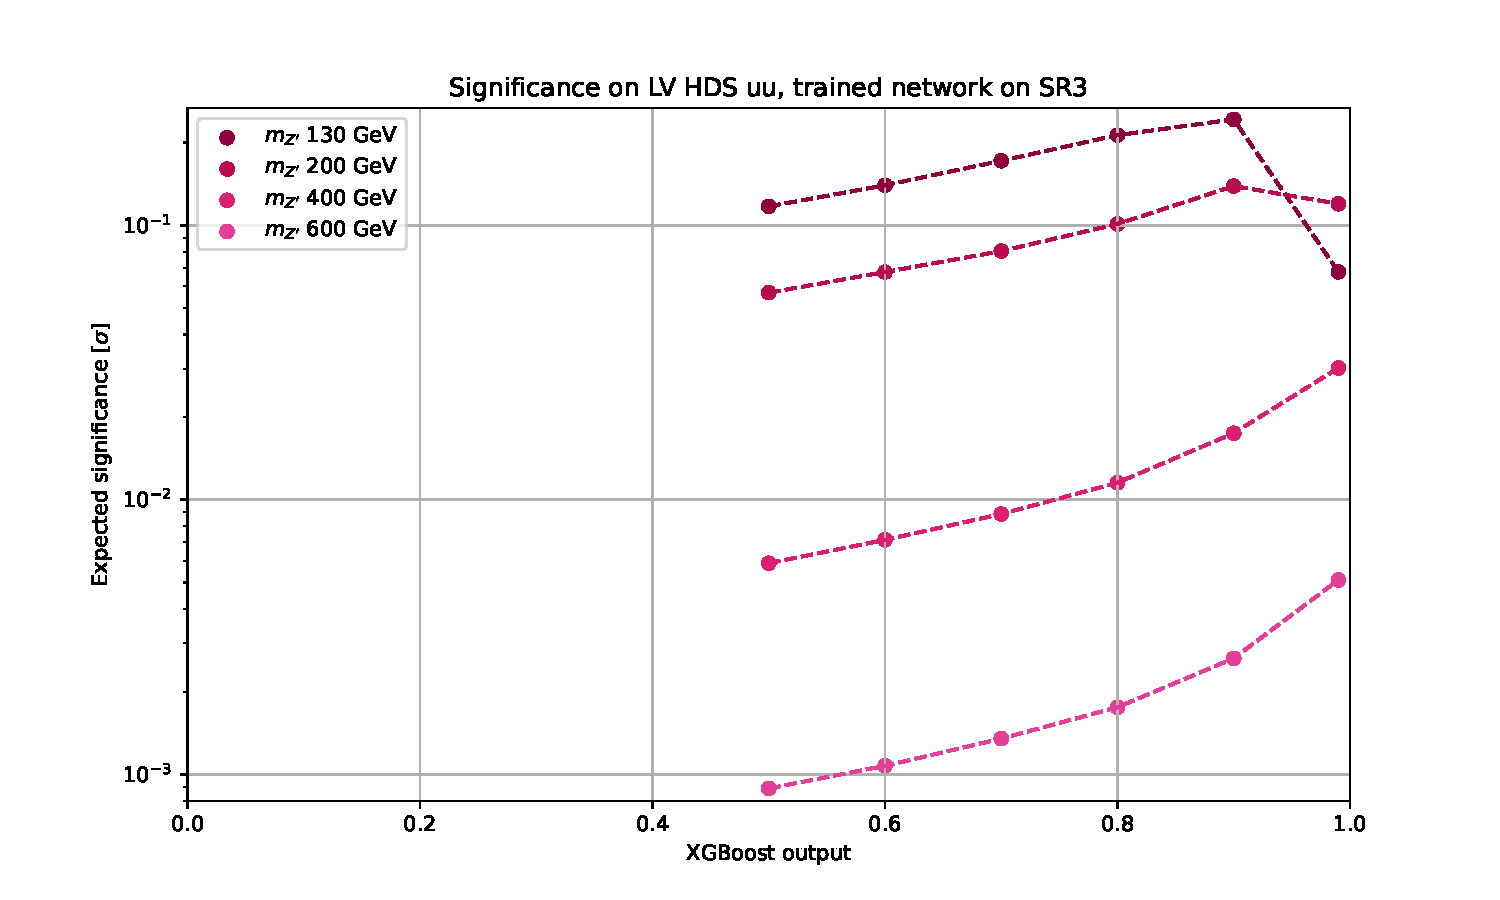
\includegraphics[width=1\textwidth]{XGBoost/Model_independent/150/LV_HDS/EXP_SIG_uu.pdf}
   \end{subfigure}
   \caption{XGBoost results for LV HDS model on $ee$ and $\mu\mu$ channel in SR3}\label{fig:LV_HDS_SR3}
\end{figure}

\begin{figure}[!ht]
	\centering
	\begin{subfigure}[b]{0.49\textwidth}
      \centering
      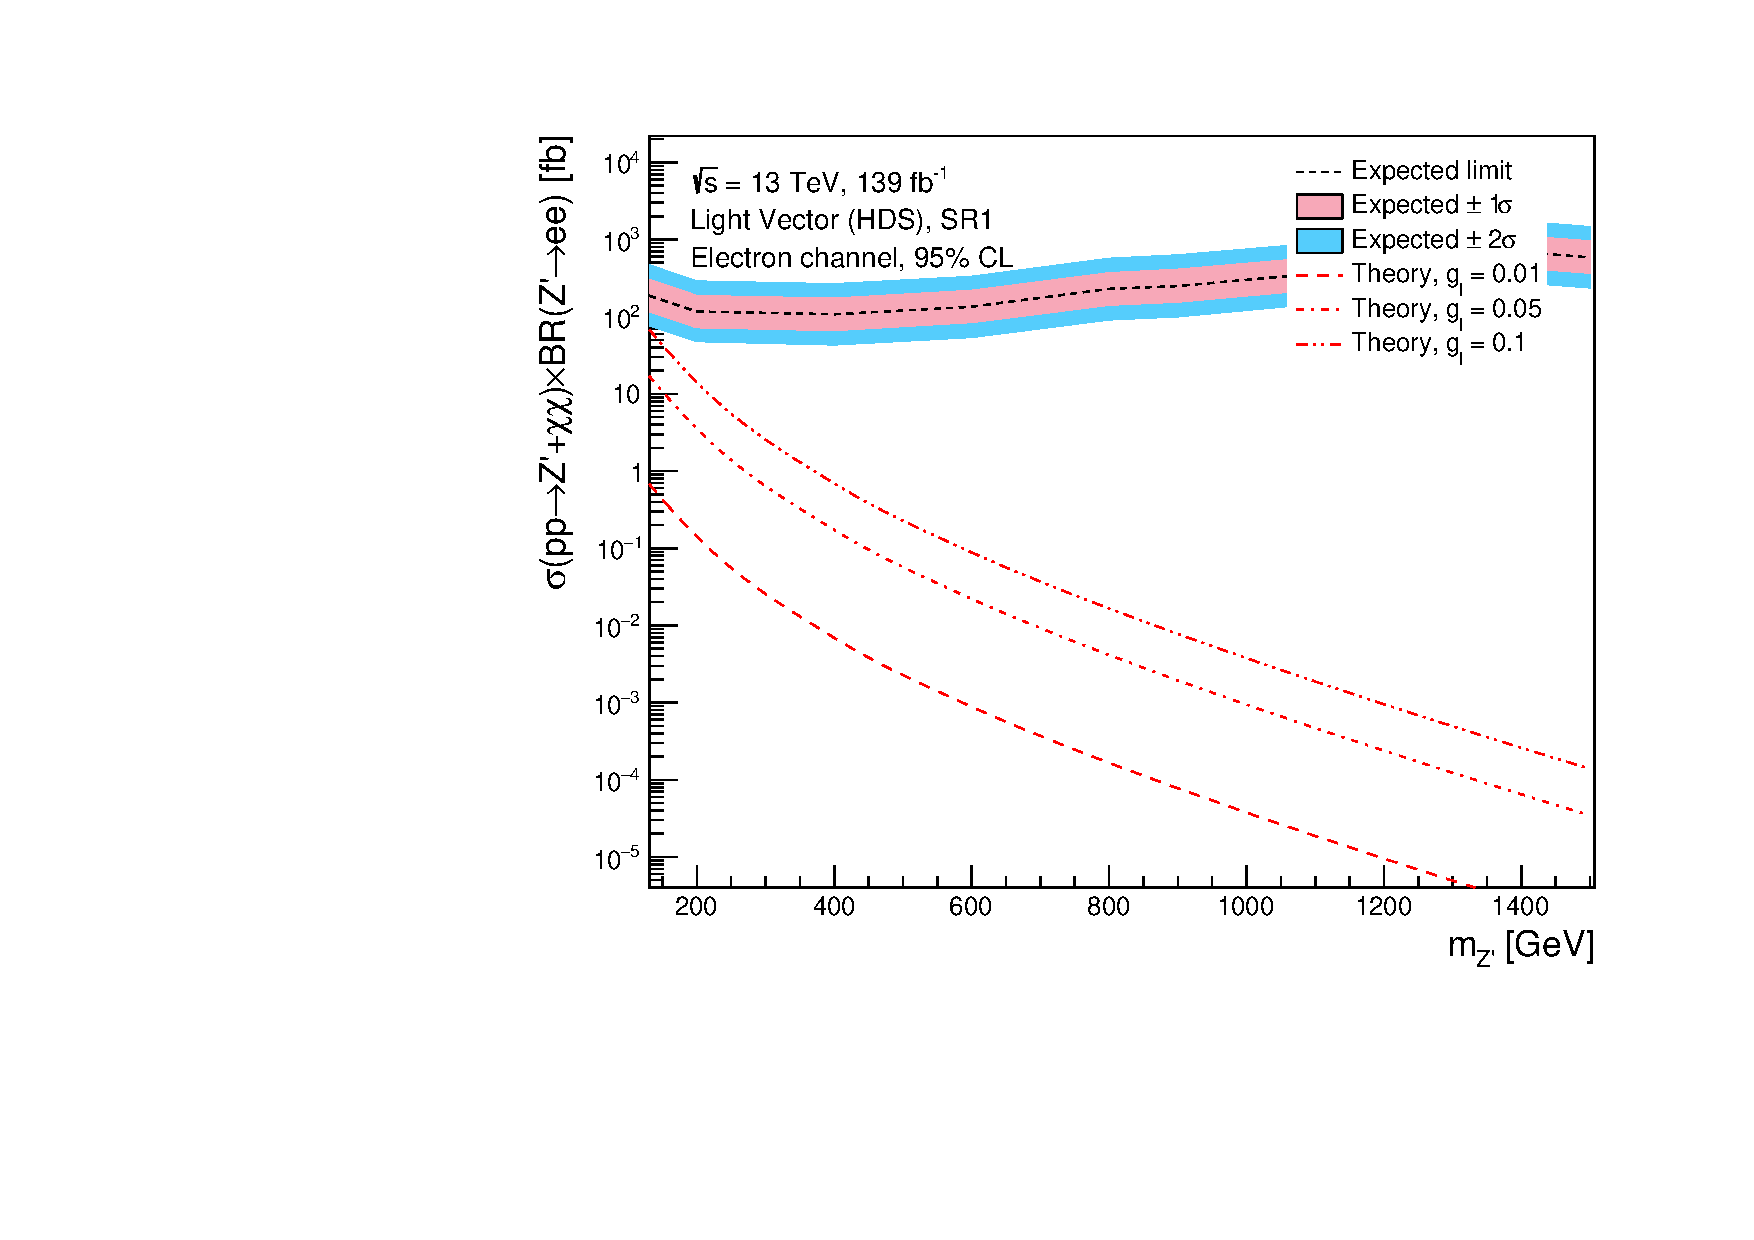
\includegraphics[width=1\textwidth]{Limits/Model_independent/50-100/LV_HDS/mass_exclusion_ee.pdf}
   \end{subfigure}
   \hfill
   \begin{subfigure}[b]{0.49\textwidth}
      \centering
      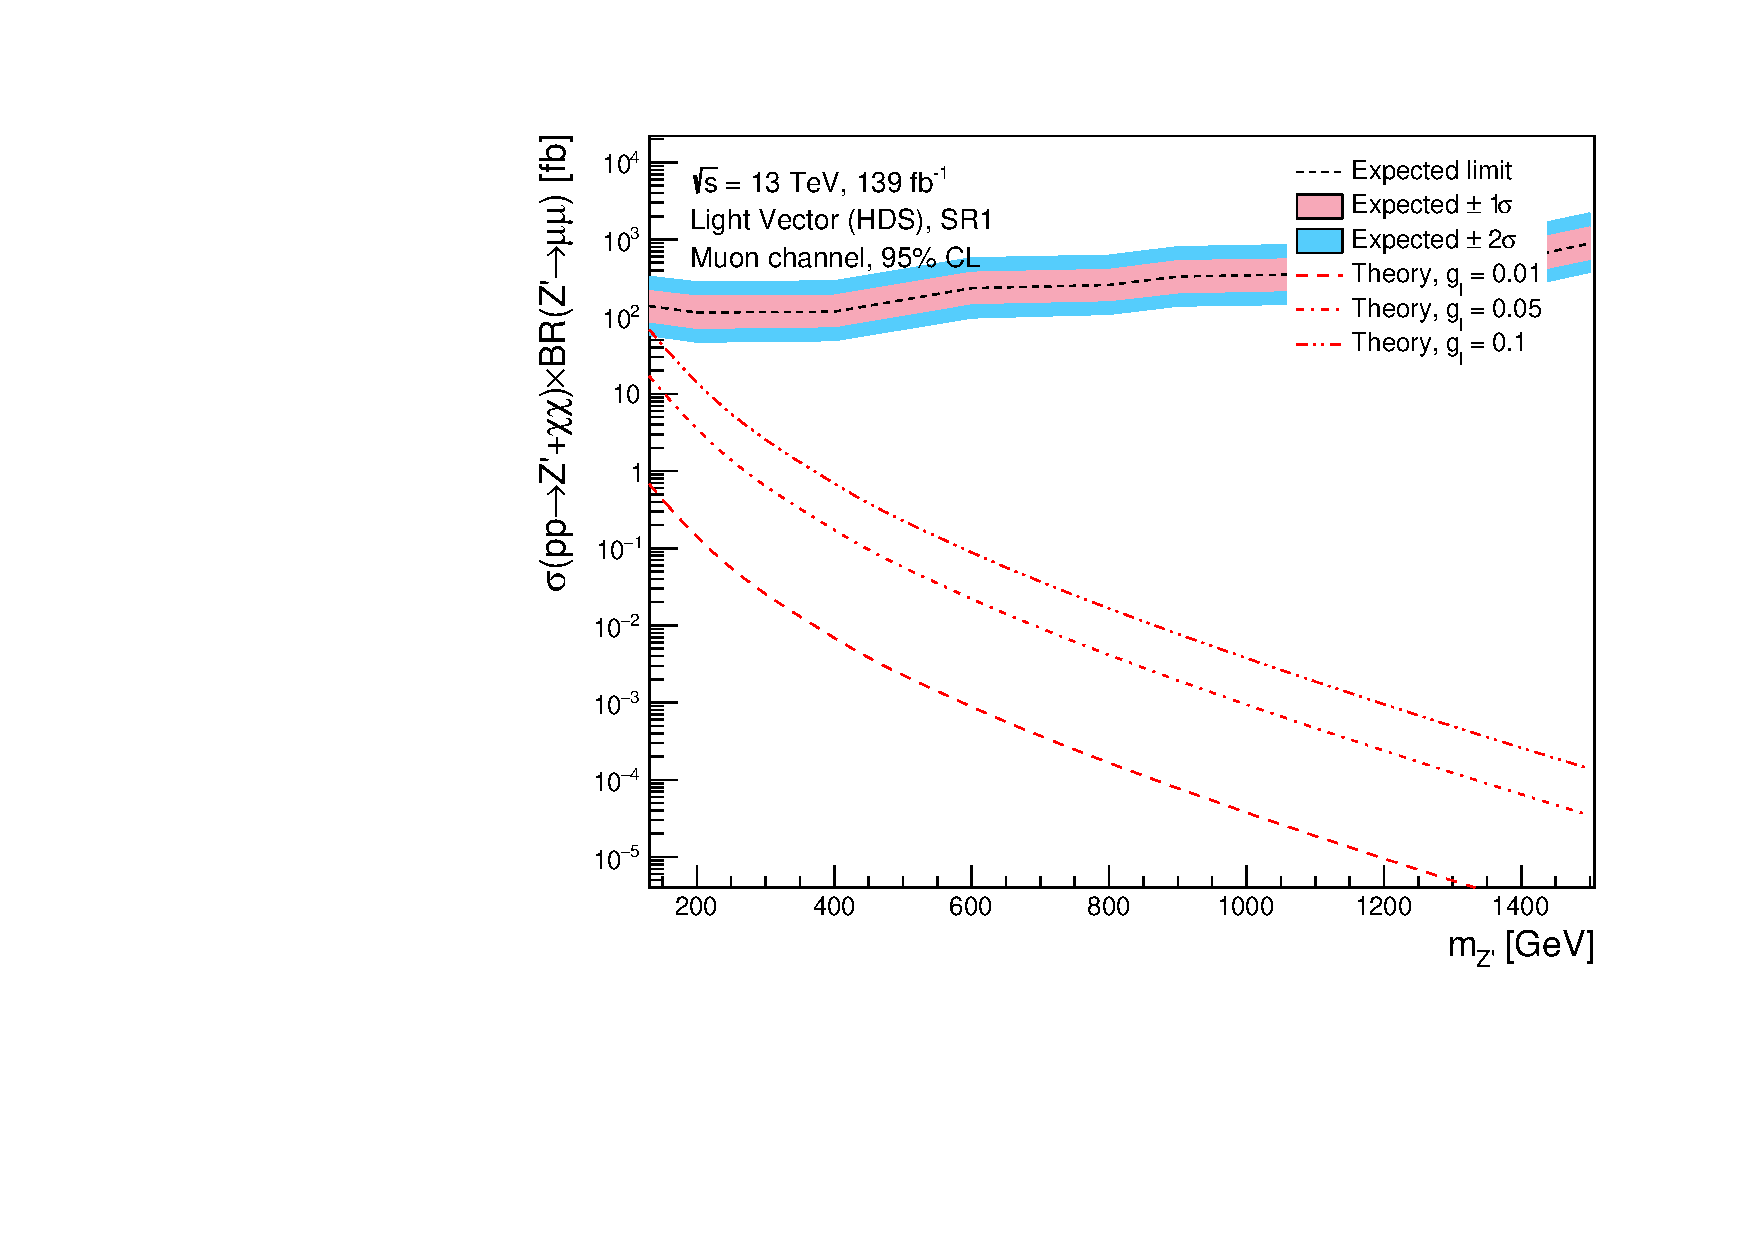
\includegraphics[width=1\textwidth]{Limits/Model_independent/50-100/LV_HDS/mass_exclusion_uu.pdf}
   \end{subfigure}
   \hfill
   \begin{subfigure}[b]{0.49\textwidth}
      \centering
      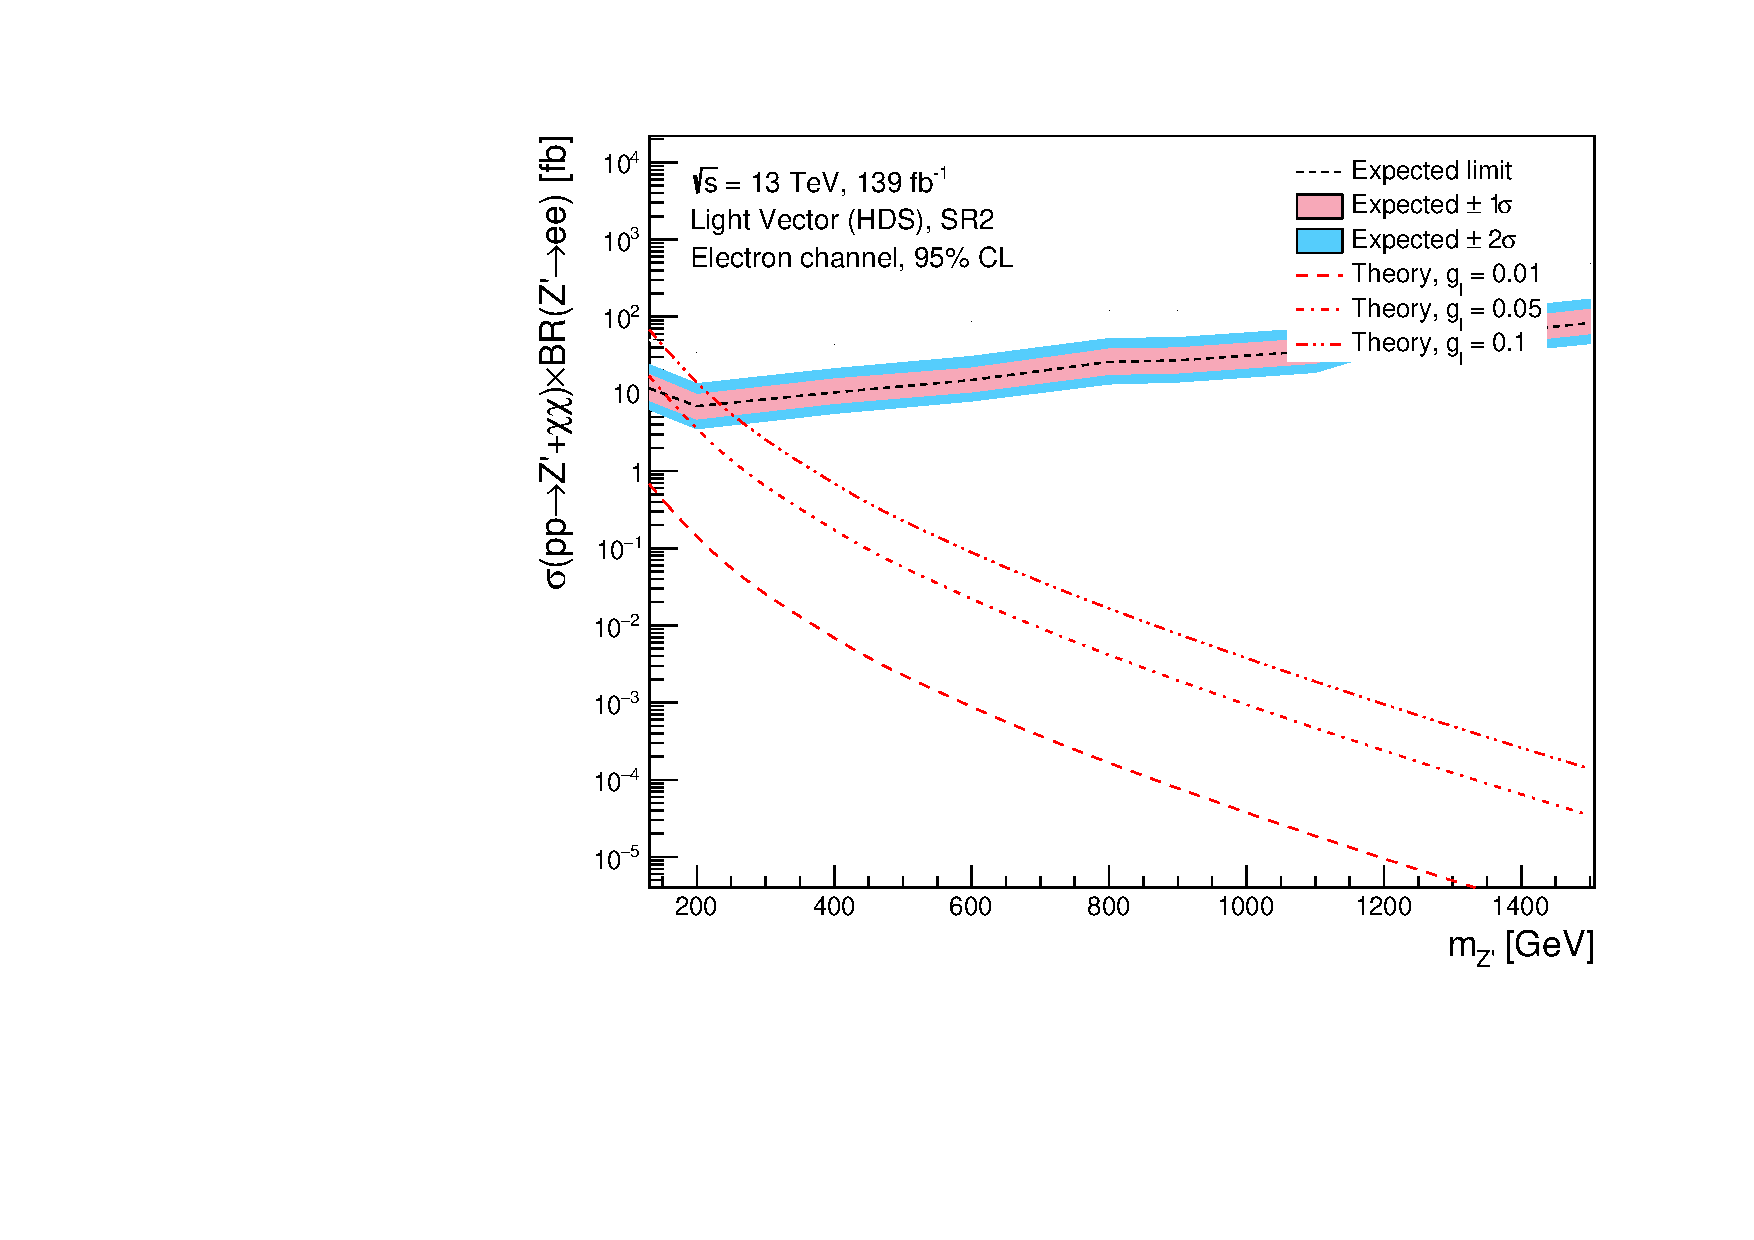
\includegraphics[width=1\textwidth]{Limits/Model_independent/100-150/LV_HDS/mass_exclusion_ee.pdf}
   \end{subfigure}
   \hfill
   \begin{subfigure}[b]{0.49\textwidth}
      \centering
      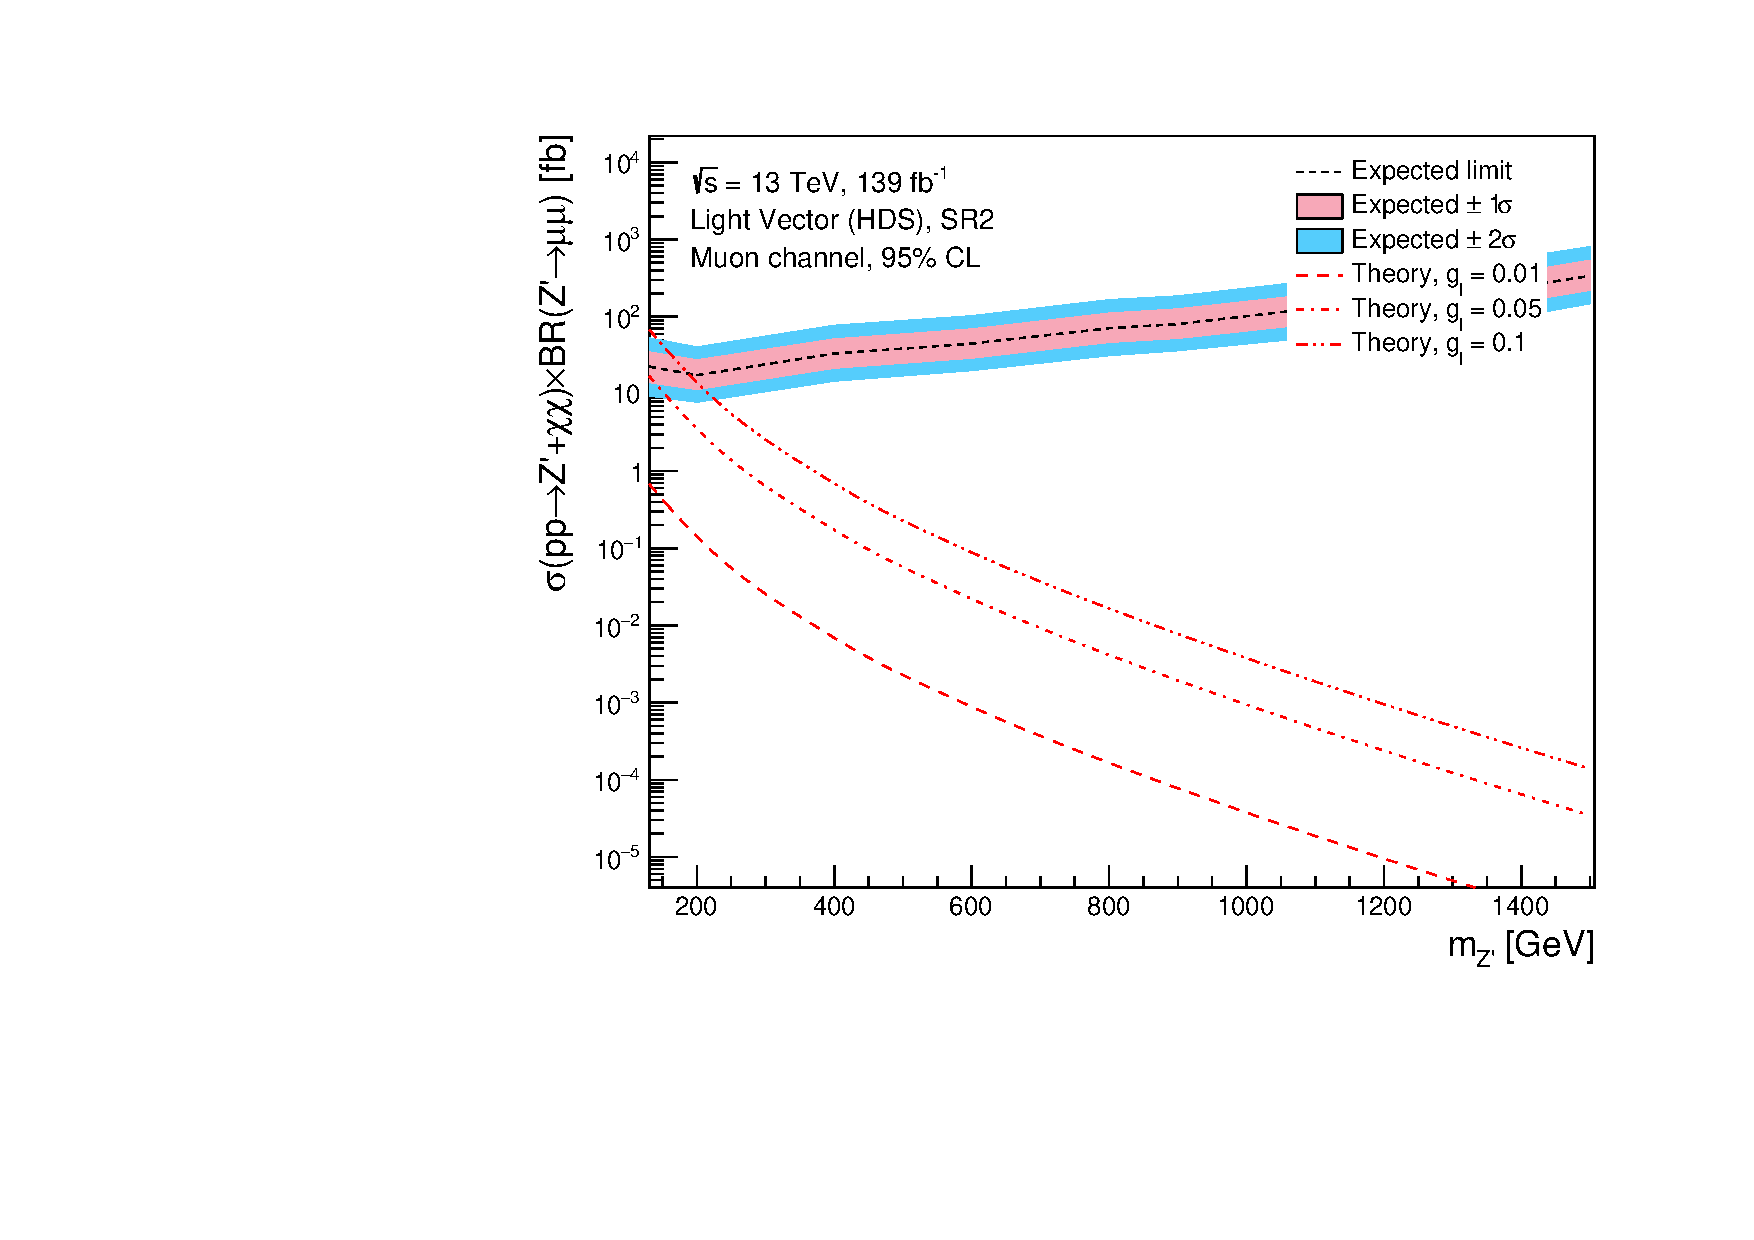
\includegraphics[width=1\textwidth]{Limits/Model_independent/100-150/LV_HDS/mass_exclusion_uu.pdf}
   \end{subfigure}
   \hfill
	\begin{subfigure}[b]{0.49\textwidth}
      \centering
      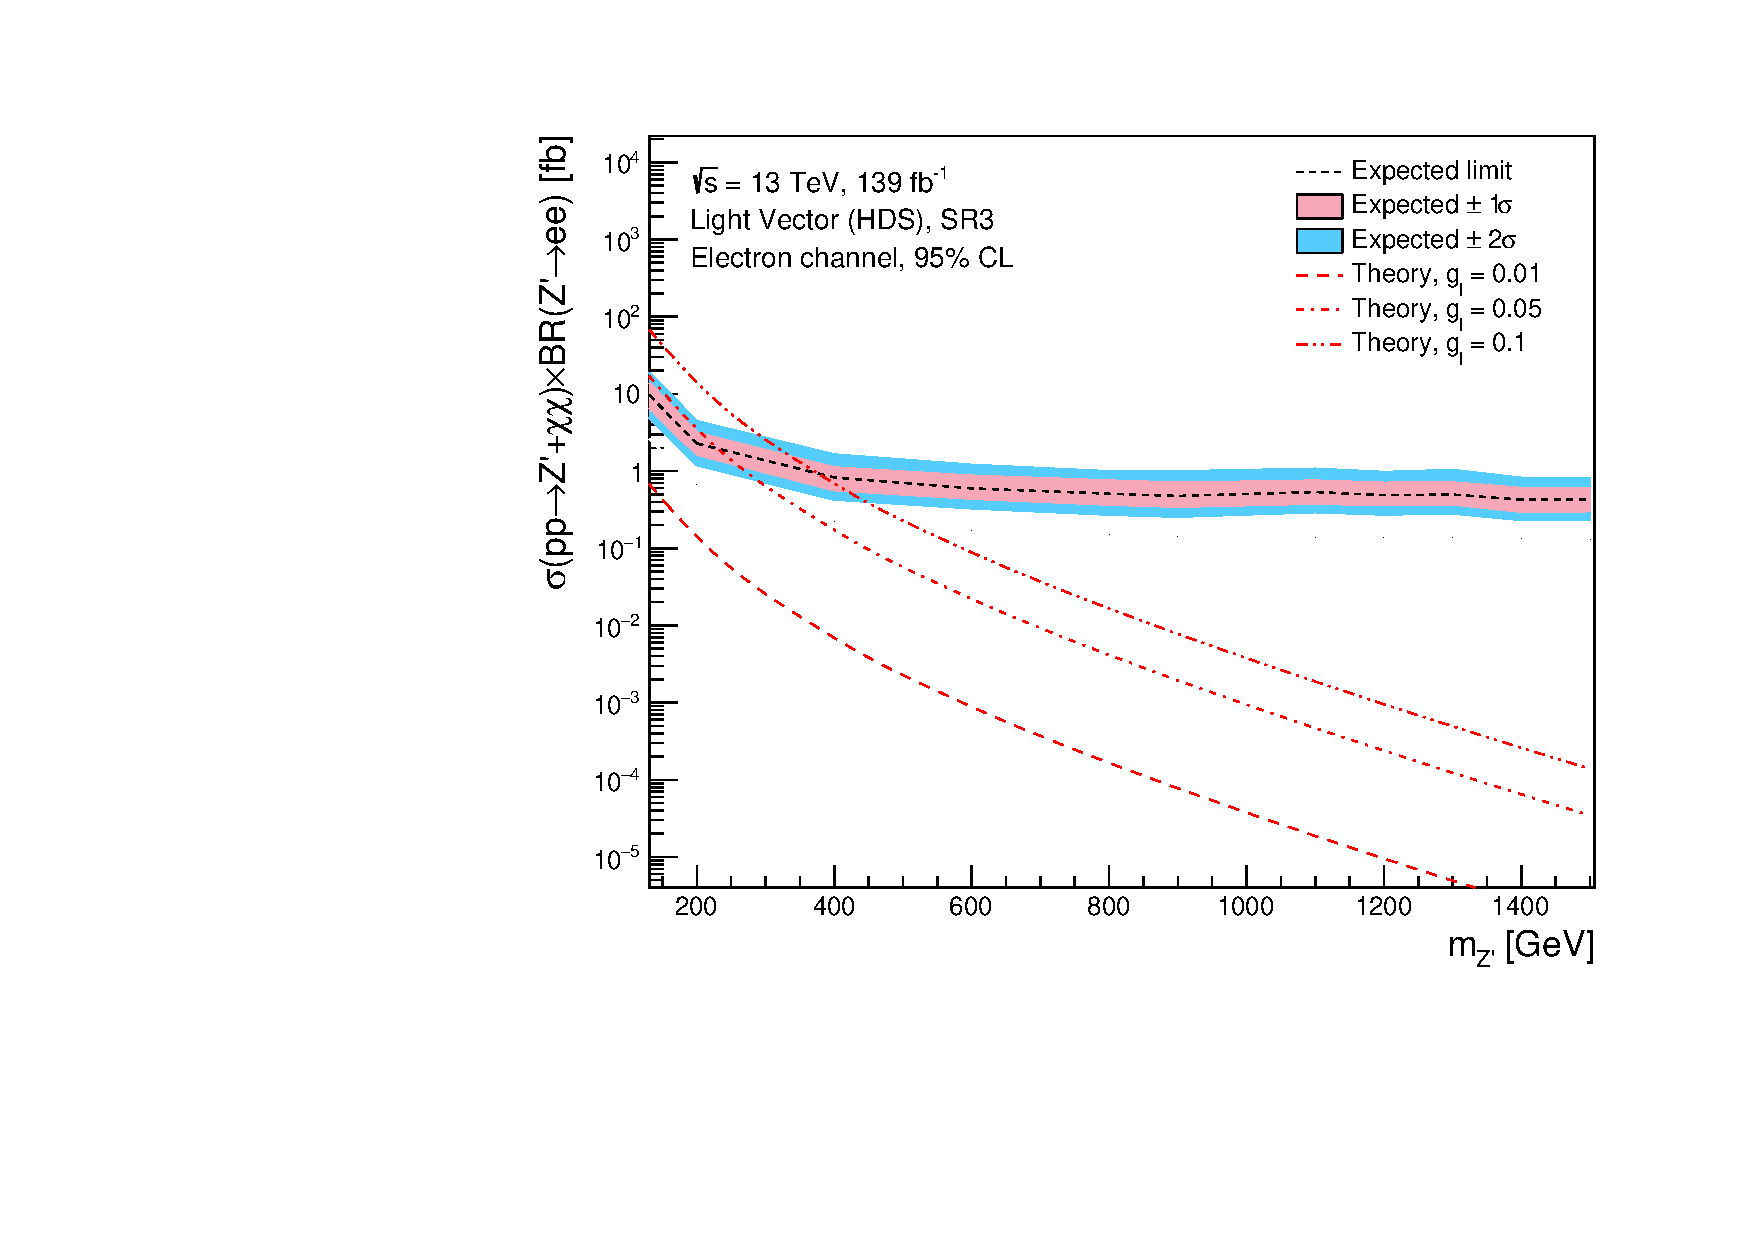
\includegraphics[width=1\textwidth]{Limits/Model_independent/150/LV_HDS/mass_exclusion_ee.pdf}
   \end{subfigure}
   \hfill
   \begin{subfigure}[b]{0.49\textwidth}
      \centering
      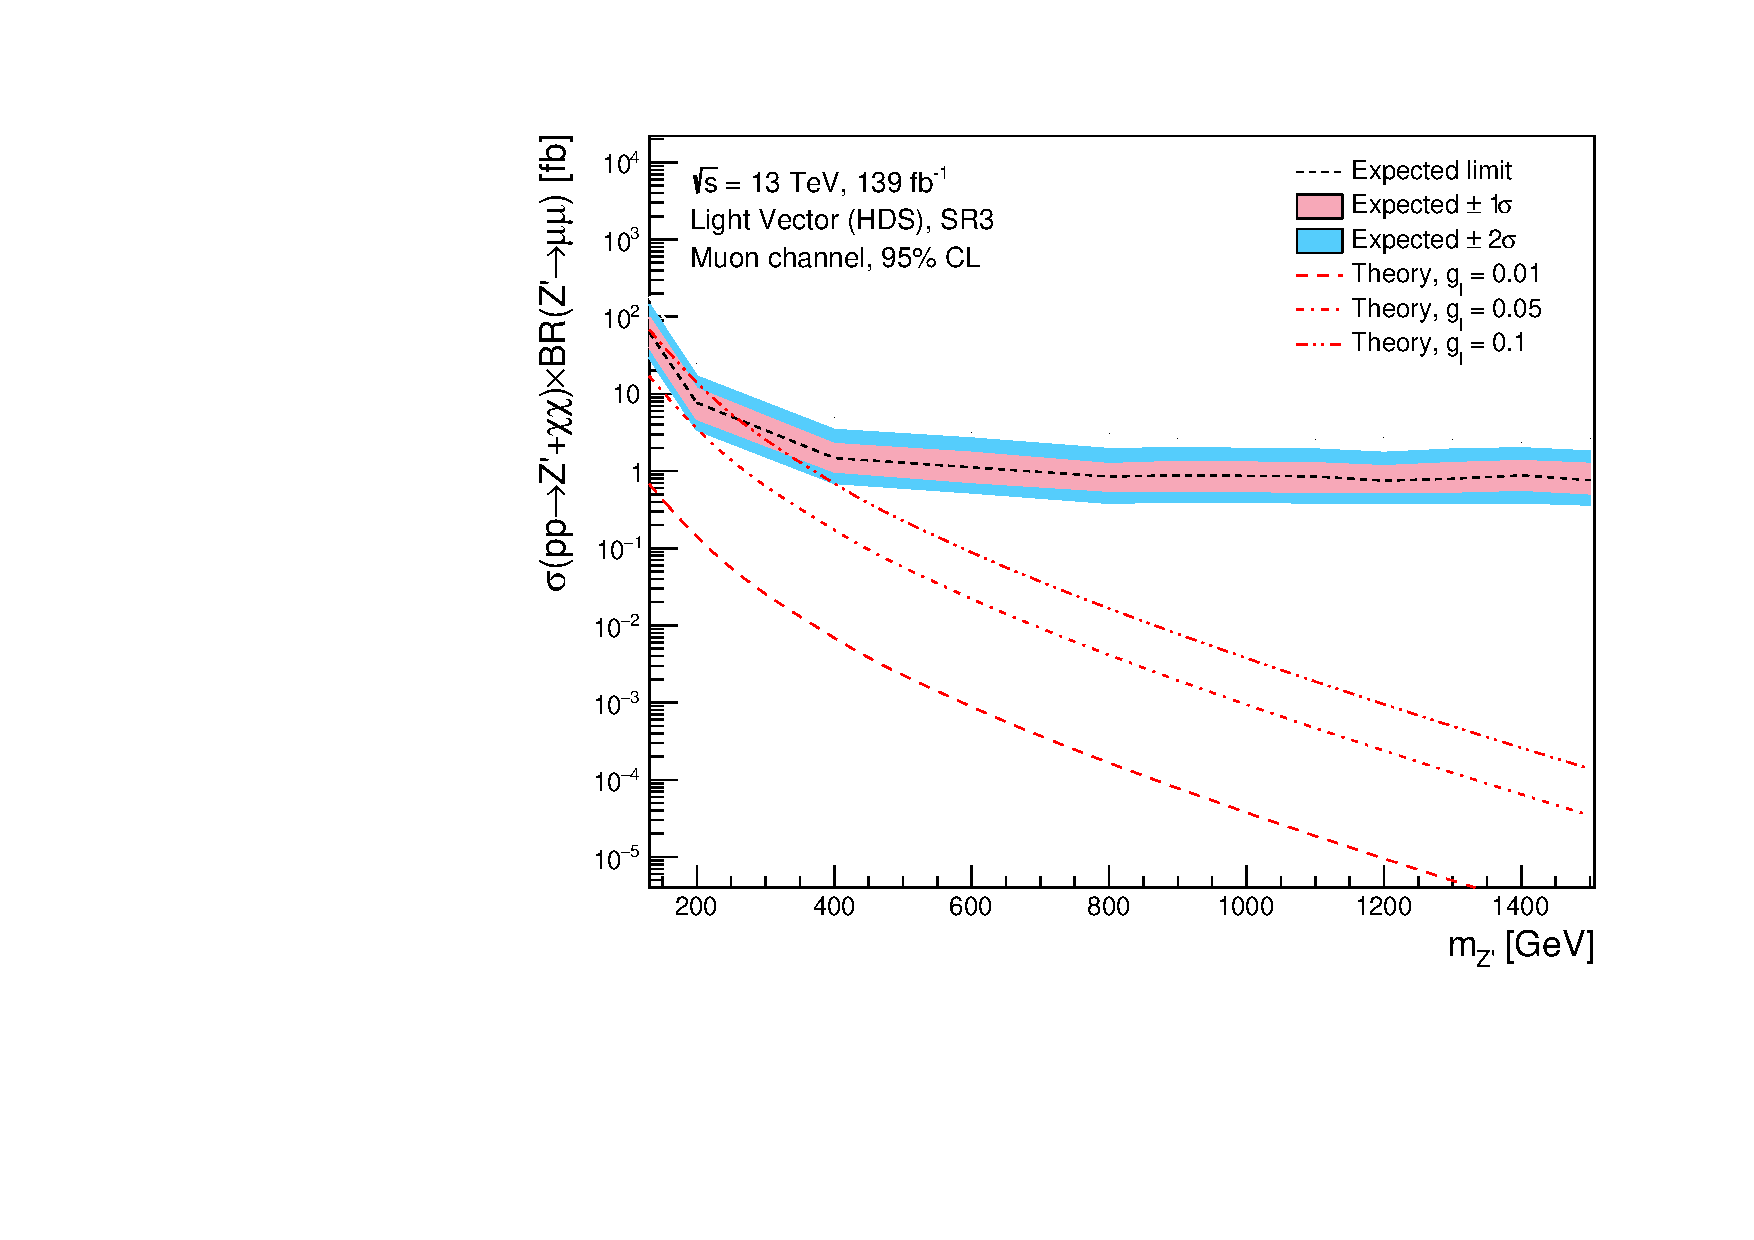
\includegraphics[width=1\textwidth]{Limits/Model_independent/150/LV_HDS/mass_exclusion_uu.pdf}
   \end{subfigure}
   \caption{Mass exclusiion limits results for LV HDS model on $ee$ and $\mu\mu$ channel in all SRs}\label{fig:LV_HDS_me_SRS}
\end{figure}

\begin{figure}[!ht]
	\centering
	\begin{subfigure}[b]{0.49\textwidth}
      \centering
      \includegraphics[width=1\textwidth]{Limits/Model_independent/LV_HDS/mass_exclusion_ee.pdf}
   \end{subfigure}
   \hfill
   \begin{subfigure}[b]{0.49\textwidth}
      \centering
      \includegraphics[width=1\textwidth]{Limits/Model_independent/LV_HDS/mass_exclusion_uu.pdf}
   \end{subfigure}
   \caption{Mass exclusiion limits results for LV HDS model on $ee$ and $\mu\mu$ channel in combined SRs}\label{fig:LV_HDS_me_comb}
\end{figure}
\clearpage
\section{Light Vector Light Dark Sector}
\begin{figure}[!ht]
	\centering
	\begin{subfigure}[b]{0.49\textwidth}
      \centering
      \includegraphics[width=1\textwidth]{XGBoost/Model_independent/50-100/LV_LDS/VAL_ee.pdf}
   \end{subfigure}
   \hfill
   \begin{subfigure}[b]{0.49\textwidth}
      \centering
      \includegraphics[width=1\textwidth]{XGBoost/Model_independent/50-100/LV_LDS/VAL_uu.pdf}
   \end{subfigure}
   \hfill
   \begin{subfigure}[b]{0.49\textwidth}
      \centering
      \includegraphics[width=1\textwidth]{XGBoost/Model_independent/50-100/LV_LDS/ROC_ee.pdf}
   \end{subfigure}
   \hfill
   \begin{subfigure}[b]{0.49\textwidth}
      \centering
      \includegraphics[width=1\textwidth]{XGBoost/Model_independent/50-100/LV_LDS/ROC_uu.pdf}
   \end{subfigure}
   \hfill
	\begin{subfigure}[b]{0.49\textwidth}
      \centering
      \includegraphics[width=1\textwidth]{XGBoost/Model_independent/50-100/LV_LDS/EXP_SIG_ee.pdf}
   \end{subfigure}
   \hfill
   \begin{subfigure}[b]{0.49\textwidth}
      \centering
      \includegraphics[width=1\textwidth]{XGBoost/Model_independent/50-100/LV_LDS/EXP_SIG_uu.pdf}
   \end{subfigure}
   \caption{XGBoost results for LV LDS model on $ee$ and $\mu\mu$ channel in SR1}\label{fig:LV_LDS_SR1}
\end{figure}

\begin{figure}[!ht]
	\centering
	\begin{subfigure}[b]{0.49\textwidth}
      \centering
      \includegraphics[width=1\textwidth]{XGBoost/Model_independent/100-150/LV_LDS/VAL_ee.pdf}
   \end{subfigure}
   \hfill
   \begin{subfigure}[b]{0.49\textwidth}
      \centering
      \includegraphics[width=1\textwidth]{XGBoost/Model_independent/100-150/LV_LDS/VAL_uu.pdf}
   \end{subfigure}
   \hfill
   \begin{subfigure}[b]{0.49\textwidth}
      \centering
      \includegraphics[width=1\textwidth]{XGBoost/Model_independent/100-150/LV_LDS/ROC_ee.pdf}
   \end{subfigure}
   \hfill
   \begin{subfigure}[b]{0.49\textwidth}
      \centering
      \includegraphics[width=1\textwidth]{XGBoost/Model_independent/100-150/LV_LDS/ROC_uu.pdf}
   \end{subfigure}
   \hfill
	\begin{subfigure}[b]{0.49\textwidth}
      \centering
      \includegraphics[width=1\textwidth]{XGBoost/Model_independent/100-150/LV_LDS/EXP_SIG_ee.pdf}
   \end{subfigure}
   \hfill
   \begin{subfigure}[b]{0.49\textwidth}
      \centering
      \includegraphics[width=1\textwidth]{XGBoost/Model_independent/100-150/LV_LDS/EXP_SIG_uu.pdf}
   \end{subfigure}
   \caption{XGBoost results for LV LDS model on $ee$ and $\mu\mu$ channel in SR2}\label{fig:LV_LDS_SR2}
\end{figure}

\begin{figure}[!ht]
	\centering
	\begin{subfigure}[b]{0.49\textwidth}
      \centering
      \includegraphics[width=1\textwidth]{XGBoost/Model_independent/150/LV_LDS/VAL_ee.pdf}
   \end{subfigure}
   \hfill
   \begin{subfigure}[b]{0.49\textwidth}
      \centering
      \includegraphics[width=1\textwidth]{XGBoost/Model_independent/150/LV_LDS/VAL_uu.pdf}
   \end{subfigure}
   \hfill
   \begin{subfigure}[b]{0.49\textwidth}
      \centering
      \includegraphics[width=1\textwidth]{XGBoost/Model_independent/150/LV_LDS/ROC_ee.pdf}
   \end{subfigure}
   \hfill
   \begin{subfigure}[b]{0.49\textwidth}
      \centering
      \includegraphics[width=1\textwidth]{XGBoost/Model_independent/150/LV_LDS/ROC_uu.pdf}
   \end{subfigure}
   \hfill
	\begin{subfigure}[b]{0.49\textwidth}
      \centering
      \includegraphics[width=1\textwidth]{XGBoost/Model_independent/150/LV_LDS/EXP_SIG_ee.pdf}
   \end{subfigure}
   \hfill
   \begin{subfigure}[b]{0.49\textwidth}
      \centering
      \includegraphics[width=1\textwidth]{XGBoost/Model_independent/150/LV_LDS/EXP_SIG_uu.pdf}
   \end{subfigure}
   \caption{XGBoost results for LV LDS model on $ee$ and $\mu\mu$ channel in SR3}\label{fig:LV_LDS_SR3}
\end{figure}

\begin{figure}[!ht]
	\centering
	\begin{subfigure}[b]{0.49\textwidth}
      \centering
      \includegraphics[width=1\textwidth]{Limits/Model_independent/50-100/LV_LDS/mass_exclusion_ee.pdf}
   \end{subfigure}
   \hfill
   \begin{subfigure}[b]{0.49\textwidth}
      \centering
      \includegraphics[width=1\textwidth]{Limits/Model_independent/50-100/LV_LDS/mass_exclusion_uu.pdf}
   \end{subfigure}
   \hfill
   \begin{subfigure}[b]{0.49\textwidth}
      \centering
      \includegraphics[width=1\textwidth]{Limits/Model_independent/100-150/LV_LDS/mass_exclusion_ee.pdf}
   \end{subfigure}
   \hfill
   \begin{subfigure}[b]{0.49\textwidth}
      \centering
      \includegraphics[width=1\textwidth]{Limits/Model_independent/100-150/LV_LDS/mass_exclusion_uu.pdf}
   \end{subfigure}
   \hfill
	\begin{subfigure}[b]{0.49\textwidth}
      \centering
      \includegraphics[width=1\textwidth]{Limits/Model_independent/150/LV_LDS/mass_exclusion_ee.pdf}
   \end{subfigure}
   \hfill
   \begin{subfigure}[b]{0.49\textwidth}
      \centering
      \includegraphics[width=1\textwidth]{Limits/Model_independent/150/LV_LDS/mass_exclusion_uu.pdf}
   \end{subfigure}
   \caption{Mass exclusiion limits results for LV LDS model on $ee$ and $\mu\mu$ channel in all SRs}\label{fig:LV_LDS_me_SRS}
\end{figure}

\begin{figure}[!ht]
	\centering
	\begin{subfigure}[b]{0.49\textwidth}
      \centering
      \includegraphics[width=1\textwidth]{Limits/Model_independent/LV_LDS/mass_exclusion_ee.pdf}
   \end{subfigure}
   \hfill
   \begin{subfigure}[b]{0.49\textwidth}
      \centering
      \includegraphics[width=1\textwidth]{Limits/Model_independent/LV_LDS/mass_exclusion_uu.pdf}
   \end{subfigure}
   \caption{Mass exclusiion limits results for LV LDS model on $ee$ and $\mu\mu$ channel in combined SRs}\label{fig:LV_LDS_me_comb}
\end{figure}
\clearpage
\section{Effective Field Theory Heavy Dark Sector}
\begin{figure}[!ht]
	\centering
	\begin{subfigure}[b]{0.49\textwidth}
      \centering
      \includegraphics[width=1\textwidth]{XGBoost/Model_independent/50-100/EFT_HDS/VAL_ee.pdf}
   \end{subfigure}
   \hfill
   \begin{subfigure}[b]{0.49\textwidth}
      \centering
      \includegraphics[width=1\textwidth]{XGBoost/Model_independent/50-100/EFT_HDS/VAL_uu.pdf}
   \end{subfigure}
   \hfill
   \begin{subfigure}[b]{0.49\textwidth}
      \centering
      \includegraphics[width=1\textwidth]{XGBoost/Model_independent/50-100/EFT_HDS/ROC_ee.pdf}
   \end{subfigure}
   \hfill
   \begin{subfigure}[b]{0.49\textwidth}
      \centering
      \includegraphics[width=1\textwidth]{XGBoost/Model_independent/50-100/EFT_HDS/ROC_uu.pdf}
   \end{subfigure}
   \hfill
	\begin{subfigure}[b]{0.49\textwidth}
      \centering
      \includegraphics[width=1\textwidth]{XGBoost/Model_independent/50-100/EFT_HDS/EXP_SIG_ee.pdf}
   \end{subfigure}
   \hfill
   \begin{subfigure}[b]{0.49\textwidth}
      \centering
      \includegraphics[width=1\textwidth]{XGBoost/Model_independent/50-100/EFT_HDS/EXP_SIG_uu.pdf}
   \end{subfigure}
   \caption{XGBoost results for EFT HDS model on $ee$ and $\mu\mu$ channel in SR1}\label{fig:EFT_HDS_SR1}
\end{figure}

\begin{figure}[!ht]
	\centering
	\begin{subfigure}[b]{0.49\textwidth}
      \centering
      \includegraphics[width=1\textwidth]{XGBoost/Model_independent/100-150/EFT_HDS/VAL_ee.pdf}
   \end{subfigure}
   \hfill
   \begin{subfigure}[b]{0.49\textwidth}
      \centering
      \includegraphics[width=1\textwidth]{XGBoost/Model_independent/100-150/EFT_HDS/VAL_uu.pdf}
   \end{subfigure}
   \hfill
   \begin{subfigure}[b]{0.49\textwidth}
      \centering
      \includegraphics[width=1\textwidth]{XGBoost/Model_independent/100-150/EFT_HDS/ROC_ee.pdf}
   \end{subfigure}
   \hfill
   \begin{subfigure}[b]{0.49\textwidth}
      \centering
      \includegraphics[width=1\textwidth]{XGBoost/Model_independent/100-150/EFT_HDS/ROC_uu.pdf}
   \end{subfigure}
   \hfill
	\begin{subfigure}[b]{0.49\textwidth}
      \centering
      \includegraphics[width=1\textwidth]{XGBoost/Model_independent/100-150/EFT_HDS/EXP_SIG_ee.pdf}
   \end{subfigure}
   \hfill
   \begin{subfigure}[b]{0.49\textwidth}
      \centering
      \includegraphics[width=1\textwidth]{XGBoost/Model_independent/100-150/EFT_HDS/EXP_SIG_uu.pdf}
   \end{subfigure}
   \caption{XGBoost results for EFT HDS model on $ee$ and $\mu\mu$ channel in SR2}\label{fig:EFT_HDS_SR2}
\end{figure}

\begin{figure}[!ht]
	\centering
	\begin{subfigure}[b]{0.49\textwidth}
      \centering
      \includegraphics[width=1\textwidth]{XGBoost/Model_independent/150/EFT_HDS/VAL_ee.pdf}
   \end{subfigure}
   \hfill
   \begin{subfigure}[b]{0.49\textwidth}
      \centering
      \includegraphics[width=1\textwidth]{XGBoost/Model_independent/150/EFT_HDS/VAL_uu.pdf}
   \end{subfigure}
   \hfill
   \begin{subfigure}[b]{0.49\textwidth}
      \centering
      \includegraphics[width=1\textwidth]{XGBoost/Model_independent/150/EFT_HDS/ROC_ee.pdf}
   \end{subfigure}
   \hfill
   \begin{subfigure}[b]{0.49\textwidth}
      \centering
      \includegraphics[width=1\textwidth]{XGBoost/Model_independent/150/EFT_HDS/ROC_uu.pdf}
   \end{subfigure}
   \hfill
	\begin{subfigure}[b]{0.49\textwidth}
      \centering
      \includegraphics[width=1\textwidth]{XGBoost/Model_independent/150/EFT_HDS/EXP_SIG_ee.pdf}
   \end{subfigure}
   \hfill
   \begin{subfigure}[b]{0.49\textwidth}
      \centering
      \includegraphics[width=1\textwidth]{XGBoost/Model_independent/150/EFT_HDS/EXP_SIG_uu.pdf}
   \end{subfigure}
   \caption{XGBoost results for EFT HDS model on $ee$ and $\mu\mu$ channel in SR3}\label{fig:EFT_HDS_SR3}
\end{figure}
\begin{figure}[!ht]
	\centering
	\begin{subfigure}[b]{0.49\textwidth}
      \centering
      \includegraphics[width=1\textwidth]{Limits/Model_independent/50-100/EFT_HDS/mass_exclusion_ee.pdf}
   \end{subfigure}
   \hfill
   \begin{subfigure}[b]{0.49\textwidth}
      \centering
      \includegraphics[width=1\textwidth]{Limits/Model_independent/50-100/EFT_HDS/mass_exclusion_uu.pdf}
   \end{subfigure}
   \hfill
   \begin{subfigure}[b]{0.49\textwidth}
      \centering
      \includegraphics[width=1\textwidth]{Limits/Model_independent/100-150/EFT_HDS/mass_exclusion_ee.pdf}
   \end{subfigure}
   \hfill
   \begin{subfigure}[b]{0.49\textwidth}
      \centering
      \includegraphics[width=1\textwidth]{Limits/Model_independent/100-150/EFT_HDS/mass_exclusion_uu.pdf}
   \end{subfigure}
   \hfill
	\begin{subfigure}[b]{0.49\textwidth}
      \centering
      \includegraphics[width=1\textwidth]{Limits/Model_independent/150/EFT_HDS/mass_exclusion_ee.pdf}
   \end{subfigure}
   \hfill
   \begin{subfigure}[b]{0.49\textwidth}
      \centering
      \includegraphics[width=1\textwidth]{Limits/Model_independent/150/EFT_HDS/mass_exclusion_uu.pdf}
   \end{subfigure}
   \caption{Mass exclusiion limits results for EFT HDS model on $ee$ and $\mu\mu$ channel in all SRs}\label{fig:EFT_HDS_me_SRS}
\end{figure}

\begin{figure}[!ht]
	\centering
	\begin{subfigure}[b]{0.49\textwidth}
      \centering
      \includegraphics[width=1\textwidth]{Limits/Model_independent/EFT_HDS/mass_exclusion_ee.pdf}
   \end{subfigure}
   \hfill
   \begin{subfigure}[b]{0.49\textwidth}
      \centering
      \includegraphics[width=1\textwidth]{Limits/Model_independent/EFT_HDS/mass_exclusion_uu.pdf}
   \end{subfigure}
   \caption{Mass exclusiion limits results for EFT HDS model on $ee$ and $\mu\mu$ channel in combined SRs}\label{fig:EFT_HDS_me_comb}
\end{figure}
\clearpage


\section{Effective Field Theory Light Dark Sector}
\begin{figure}[!ht]
	\centering
	\begin{subfigure}[b]{0.49\textwidth}
      \centering
      \includegraphics[width=1\textwidth]{XGBoost/Model_independent/50-100/EFT_LDS/VAL_ee.pdf}
   \end{subfigure}
   \hfill
   \begin{subfigure}[b]{0.49\textwidth}
      \centering
      \includegraphics[width=1\textwidth]{XGBoost/Model_independent/50-100/EFT_LDS/VAL_uu.pdf}
   \end{subfigure}
   \hfill
   \begin{subfigure}[b]{0.49\textwidth}
      \centering
      \includegraphics[width=1\textwidth]{XGBoost/Model_independent/50-100/EFT_LDS/ROC_ee.pdf}
   \end{subfigure}
   \hfill
   \begin{subfigure}[b]{0.49\textwidth}
      \centering
      \includegraphics[width=1\textwidth]{XGBoost/Model_independent/50-100/EFT_LDS/ROC_uu.pdf}
   \end{subfigure}
   \hfill
	\begin{subfigure}[b]{0.49\textwidth}
      \centering
      \includegraphics[width=1\textwidth]{XGBoost/Model_independent/50-100/EFT_LDS/EXP_SIG_ee.pdf}
   \end{subfigure}
   \hfill
   \begin{subfigure}[b]{0.49\textwidth}
      \centering
      \includegraphics[width=1\textwidth]{XGBoost/Model_independent/50-100/EFT_LDS/EXP_SIG_uu.pdf}
   \end{subfigure}
   \caption{XGBoost results for EFT LDS model on $ee$ and $\mu\mu$ channel in SR1}\label{fig:EFT_LDS_SR1}
\end{figure}

\begin{figure}[!ht]
	\centering
	\begin{subfigure}[b]{0.49\textwidth}
      \centering
      \includegraphics[width=1\textwidth]{XGBoost/Model_independent/100-150/EFT_LDS/VAL_ee.pdf}
   \end{subfigure}
   \hfill
   \begin{subfigure}[b]{0.49\textwidth}
      \centering
      \includegraphics[width=1\textwidth]{XGBoost/Model_independent/100-150/EFT_LDS/VAL_uu.pdf}
   \end{subfigure}
   \hfill
   \begin{subfigure}[b]{0.49\textwidth}
      \centering
      \includegraphics[width=1\textwidth]{XGBoost/Model_independent/100-150/EFT_LDS/ROC_ee.pdf}
   \end{subfigure}
   \hfill
   \begin{subfigure}[b]{0.49\textwidth}
      \centering
      \includegraphics[width=1\textwidth]{XGBoost/Model_independent/100-150/EFT_LDS/ROC_uu.pdf}
   \end{subfigure}
   \hfill
	\begin{subfigure}[b]{0.49\textwidth}
      \centering
      \includegraphics[width=1\textwidth]{XGBoost/Model_independent/100-150/EFT_LDS/EXP_SIG_ee.pdf}
   \end{subfigure}
   \hfill
   \begin{subfigure}[b]{0.49\textwidth}
      \centering
      \includegraphics[width=1\textwidth]{XGBoost/Model_independent/100-150/EFT_LDS/EXP_SIG_uu.pdf}
   \end{subfigure}
   \caption{XGBoost results for EFT LDS model on $ee$ and $\mu\mu$ channel in SR2}\label{fig:EFT_LDS_SR2}
\end{figure}

\begin{figure}[!ht]
	\centering
	\begin{subfigure}[b]{0.49\textwidth}
      \centering
      \includegraphics[width=1\textwidth]{XGBoost/Model_independent/150/EFT_LDS/VAL_ee.pdf}
   \end{subfigure}
   \hfill
   \begin{subfigure}[b]{0.49\textwidth}
      \centering
      \includegraphics[width=1\textwidth]{XGBoost/Model_independent/150/EFT_LDS/VAL_uu.pdf}
   \end{subfigure}
   \hfill
   \begin{subfigure}[b]{0.49\textwidth}
      \centering
      \includegraphics[width=1\textwidth]{XGBoost/Model_independent/150/EFT_LDS/ROC_ee.pdf}
   \end{subfigure}
   \hfill
   \begin{subfigure}[b]{0.49\textwidth}
      \centering
      \includegraphics[width=1\textwidth]{XGBoost/Model_independent/150/EFT_LDS/ROC_uu.pdf}
   \end{subfigure}
   \hfill
	\begin{subfigure}[b]{0.49\textwidth}
      \centering
      \includegraphics[width=1\textwidth]{XGBoost/Model_independent/150/EFT_LDS/EXP_SIG_ee.pdf}
   \end{subfigure}
   \hfill
   \begin{subfigure}[b]{0.49\textwidth}
      \centering
      \includegraphics[width=1\textwidth]{XGBoost/Model_independent/150/EFT_LDS/EXP_SIG_uu.pdf}
   \end{subfigure}
   \caption{XGBoost results for EFT LDS model on $ee$ and $\mu\mu$ channel in SR3}\label{fig:EFT_LDS_SR3}
\end{figure}
\begin{figure}[!ht]
	\centering
	\begin{subfigure}[b]{0.49\textwidth}
      \centering
      \includegraphics[width=1\textwidth]{Limits/Model_independent/50-100/EFT_LDS/mass_exclusion_ee.pdf}
   \end{subfigure}
   \hfill
   \begin{subfigure}[b]{0.49\textwidth}
      \centering
      \includegraphics[width=1\textwidth]{Limits/Model_independent/50-100/EFT_LDS/mass_exclusion_uu.pdf}
   \end{subfigure}
   \hfill
   \begin{subfigure}[b]{0.49\textwidth}
      \centering
      \includegraphics[width=1\textwidth]{Limits/Model_independent/100-150/EFT_LDS/mass_exclusion_ee.pdf}
   \end{subfigure}
   \hfill
   \begin{subfigure}[b]{0.49\textwidth}
      \centering
      \includegraphics[width=1\textwidth]{Limits/Model_independent/100-150/EFT_LDS/mass_exclusion_uu.pdf}
   \end{subfigure}
   \hfill
	\begin{subfigure}[b]{0.49\textwidth}
      \centering
      \includegraphics[width=1\textwidth]{Limits/Model_independent/150/EFT_LDS/mass_exclusion_ee.pdf}
   \end{subfigure}
   \hfill
   \begin{subfigure}[b]{0.49\textwidth}
      \centering
      \includegraphics[width=1\textwidth]{Limits/Model_independent/150/EFT_LDS/mass_exclusion_uu.pdf}
   \end{subfigure}
   \caption{Mass exclusiion limits results for EFT LDS model on $ee$ and $\mu\mu$ channel in all SRs}\label{fig:EFT_LDS_me_SRS}
\end{figure}

\begin{figure}[!ht]
	\centering
	\begin{subfigure}[b]{0.49\textwidth}
      \centering
      \includegraphics[width=1\textwidth]{Limits/Model_independent/EFT_LDS/mass_exclusion_ee.pdf}
   \end{subfigure}
   \hfill
   \begin{subfigure}[b]{0.49\textwidth}
      \centering
      \includegraphics[width=1\textwidth]{Limits/Model_independent/EFT_LDS/mass_exclusion_uu.pdf}
   \end{subfigure}
   \caption{Mass exclusiion limits results for EFT LDS model on $ee$ and $\mu\mu$ channel in combined SRs}\label{fig:EFT_LDS_me_comb}
\end{figure}

\clearpage


\end{document}